%!TEX root = ../../thesis.tex
%%%% CHAPTER 0 *****************************************************************
\ifx\printIntroduction\undefined
\else
\chapter[Soft Robotics -- a new perspective]{Soft Robotics -- a new \\ perspective on biomimicry}
\label{chap: chapter 0}
\vspace*{-12mm}
%\begingroup
%\introabstract{We begin this thesis with a brief overview of the rich history of soft robotics, and its research topics. During the first part, the reader will be familiarized with the field and terminologies common to the field. We will transition from rigid to soft robotics, highlighting is early inception. Once familaizer with the field, we will discuss its academic roots, related to topics on design, modeling and control strategies.}
%\endgroup

%!TEX root = ../../thesis.tex
\section{History of soft robotics: what are they?} 
\label{sec:intro:history}
Biological systems have long been an inspiration for roboticist to make more robust and capable machines. While holding these pages in one's hand, one might wonder \textit{'how do we interact with so many different objects so effortlessly on a daily basis?'}. A conventional (rigid) robot, on the other hand, needs to know the exact weight, shape, and orientation of an object to interact with it safely and robustly. These philosophies adopted from nature are now presented into machines that accordingly shaped a new robotics discipline called \emph{soft robotics}. Contrary to rigid robots, these machines are made from softer materials. Softness here refers to the enveloping properties of low elasticity materials. Indeed, by observing common materials in robotics and their elastic moduli (see Figure \ref{fig:C0:elasticity}), we observe a gap between machine and nature. It is believed that the lack of material diversity in robotics might be the missing puzzle piece of achieving bio-like performance in modern machines.
%A common measure of the elasticity is the Young's modulus. Although it only applies to homogenous materials subject to small deformations, it can be explored to classify rigidity in robotics. To aid the reader, we have provided a spectrum of different materials in Figure \ref{fig:C0:elasticity}. Observing this spectrum, we see that biological organisms are mostly composed of materials with low moduli in the order of $10^4 - 10^7$ \si{Pa} (\eg, muscle or skin tissue) and sparsely of rigid materials, \eg, bone. Classic robotics, on the other hand, are predominantly composed of hard materials, like metals or hard plastics. 
% It is interesting to observe that the materials responsible for motion, which naturally undergo repeated deformation, have accordingly low elasticity. As opposed to the use of rigid materials in classic robotics. 
The idea of exploring low elasticity materials in robotics, so-called \textit{soft material}, has sparked a new direction in robotics aimed at harmonizing robots and biology. Before continuing, we introduce the following definition:
%
\terminology{\textbf{Soft materials} are a class of homogenous materials with a Young's modulus (\ie, the modulus of elasticity) lower than $E \le 10^9$ \si{\pascal}. Following, the word softness refers to the collection of mechanical properties that are often associated with these low moduli materials.}{}\
%
Now, although the words \emph{soft} and \emph{robotics} have a clear definition independently, the collocation of the two sparked many vivid discussions and new idealogies within the robotics community for the past two decades. Throughout its young academic life, several defintions have been coined. Early terms for soft robotics were used to indicate robots with variable joint stiffness \cite{AlbuSchaffer2004}, or artificial compliance through control \cite{AlbuSchaffer2011}. The term was also used to underline the shift from rigid-linked robots to \textit{bio-inspired continuum robots are inherently compliant and that exhibit large strains in normal operations} \cite{Trivedi2008}. Paraphrasing the work of Robison et al. (1999, \cite{Robinson1999}): \textit{soft robotic manipulators are continuum robots made of soft materials that undergo continuous elastic deformation and produce motion through the generation of a smooth backbone curve}. Alternatively, a broader definition was coined in a review by Kim et al. (\cite{Kim2013}, 2013) simply referring to soft-bodied robots as \textit{an analogy to soft-bodied animals}. A concise (but generic) definition was proposed by Laschi et al. (\cite{Laschi2014}, 2014), as soft robots being \textit{any robot built by soft materials}. Rus et al. (2015, \cite{Rus2015}) defined soft robots in terms of their structural elasticity: \textit{Systems that are capable of autonomous behavior, and that are primarily composed of materials with moduli in the range of that of soft biological materials}.
%
\begin{figure}[!t]
  \ifx\printFigures\undefined
  \else
  \centering
  \vspace{-3mm}
  % This file was created by matlab2tikz.
%
%The latest updates can be retrieved from
%  http://www.mathworks.com/matlabcentral/fileexchange/22022-matlab2tikz-matlab2tikz
%where you can also make suggestions and rate matlab2tikz.
%
\definecolor{mycolor1}{rgb}{0.00784,0.74902,0.90588}%
\definecolor{mycolor2}{rgb}{1.00000,0.16078,0.45882}%
%
\begin{tikzpicture}

\begin{axis}[%
width=0.751\textwidth,
height=0.139\textwidth,
at={(0.116\textwidth,0.002\textwidth)},
scale only axis,
xmin=0,
xmax=1,
ymin=0,
ymax=1,
axis line style={draw=none},
ticks=none,
axis x line*=bottom,
axis y line*=left
]
\end{axis}

\begin{axis}[%
width=0.95\textwidth,
height=0.075\textwidth,
at={(0\textwidth,0.077\textwidth)},
scale only axis,
xmin=0,
xmax=1,
xtick={0,0.1,0.2,0.3,0.4,0.5,0.6,0.7,0.8,0.9,1},
xticklabels={\empty},
ymin=0,
ymax=1,
ytick={0,0.5,1},
yticklabels={\empty},
axis line style={draw=none},
ticks=none,
axis x line*=bottom,
axis y line*=left
]
\end{axis}

\begin{axis}[%
width=0.95\textwidth,
height=0.075\textwidth,
at={(0\textwidth,0\textwidth)},
scale only axis,
clip=false,
xmode=log,
xmin=10000,
xmax=1100000000000,
xtick={10000,100000,1000000,10000000,100000000,1000000000,10000000000,100000000000,1000000000000},
xticklabels={{$\text{10}^{\text{4}}$},{$\text{10}^{\text{5}}$},{$\text{10}^{\text{6}}$},{$\text{10}^{\text{7}}$},{$\text{10}^{\text{8}}$},{$\text{10}^{\text{9}}$},{$\text{10}^{\text{10}}$},{$\text{10}^{\text{11}}$},{$\text{10}^{\text{12}}$}},
xminorticks=true,
ymin=-1,
ymax=1,
ytick={\empty},
axis background/.style={fill=white},
xmajorgrids,
xminorgrids,
ymajorgrids
]
\addplot [color=white, forget plot]
  table[row sep=crcr]{%
10000	0\\
12626.0010987486	0\\
15941.59037456	0\\
20127.8537584994	0\\
25413.4303670264	0\\
32086.9999737045	0\\
40513.0496923538	0\\
51151.7809929315	0\\
64584.2443019698	0\\
81544.0739518515	0\\
102957.556731251	0\\
129994.222441324	0\\
164130.719537513	0\\
207231.464521903	0\\
261650.469874882	0\\
330359.912012834	0\\
417112.461205652	0\\
526646.239348428	0\\
664943.599666505	0\\
839557.86199951	0\\
1060025.84880688	0\\
1338388.75317376	0\\
1689849.78681246	0\\
2133604.52650141	0\\
2693889.30959018	0\\
3401304.93827925	0\\
4294487.98878927	0\\
5422221.00650159	0\\
6846096.83857466	0\\
8643882.62059826	0\\
10913767.1465127	0\\
13779723.5983356	0\\
17398280.5293036	0\\
21967070.9079324	0\\
27735626.1419842	0\\
35019004.6143171	0\\
44214999.0737449	0\\
55825862.688627	0\\
70485740.364519	0\\
88995303.5288522	0\\
112365480.013875	0\\
141872667.41166	0\\
179128445.4622	0\\
226167594.922286	0\\
285559230.19901	0\\
360547115.42505	0\\
455226827.550731	0\\
574769442.483536	0\\
725703961.232423	0\\
916273901.188673	0\\
1156887528.31628	0\\
1460686320.36499	0\\
1844262708.58553	0\\
2328566298.4982	0\\
2940048064.33471	0\\
3712105009.06637	0\\
4686904192.31419	0\\
5917685748.18881	0\\
7471670675.86807	0\\
9433732216.29977	0\\
11911031332.8301	0\\
15038869469.5541	0\\
18988078244.6526	0\\
23974349678.0108	0\\
30270016537.6346	0\\
38218926206.3311	0\\
48255220427.4128	0\\
60927046613.6869	0\\
76926495748.7916	0\\
97127401984.7117	0\\
122633068417.756	0\\
154836525658.55	0\\
195496614309.126	0\\
246834046706.865	0\\
311652694492.944	0\\
393492726309.585	0\\
496823959473.439	0\\
627289985819.623	0\\
792016405019.254	0\\
1000000000000	0\\
};

\addplot[area legend, draw=none, fill=mycolor1, fill opacity=0.75, forget plot]
table[row sep=crcr] {%
x	y\\
10000	-1\\
15000	-1\\
15000	1\\
10000	1\\
}--cycle;
\node[right, align=left, rotate=70]
at (axis cs:9775,1.3) {\scriptsize Hydrogel};

\addplot[area legend, draw=none, fill=mycolor1, fill opacity=0.75, forget plot]
table[row sep=crcr] {%
x	y\\
100000	-1\\
770000	-1\\
770000	1\\
100000	1\\
}--cycle;
\node[right, align=left, rotate=70]
at (axis cs:255850,1.3) {\scriptsize Elastomer};

\addplot[area legend, draw=none, fill=mycolor2, fill opacity=0.75, forget plot]
table[row sep=crcr] {%
x	y\\
20500	-1\\
27500	-1\\
27500	1\\
20500	1\\
}--cycle;
\node[right, align=left, rotate=70]
at (axis cs:19210,1.3) {\scriptsize Skeletal muscle};

\addplot[area legend, draw=none, fill=mycolor2, fill opacity=0.75, forget plot]
table[row sep=crcr] {%
x	y\\
90000	-1\\
110000	-1\\
110000	1\\
90000	1\\
}--cycle;
\node[right, align=left, rotate=70]
at (axis cs:81600,1.3) {\scriptsize Cardiac muscle};

\addplot[area legend, draw=none, fill=mycolor2, fill opacity=0.75, forget plot]
table[row sep=crcr] {%
x	y\\
1258925.41179417	-1\\
1995262.31496888	-1\\
1995262.31496888	1\\
1258925.41179417	1\\
}--cycle;
\node[right, align=left, rotate=70]
at (axis cs:1257852.51,1.3) {\scriptsize Artery};

\addplot[area legend, draw=none, fill=mycolor1, fill opacity=0.75, forget plot]
table[row sep=crcr] {%
x	y\\
31622776.6016838	-1\\
63095734.4480193	-1\\
63095734.4480193	1\\
31622776.6016838	1\\
}--cycle;
\node[right, align=left, rotate=70]
at (axis cs:34904964.362,1.3) {\scriptsize Rubber};

\addplot[area legend, draw=none, fill=mycolor2, fill opacity=0.75, forget plot]
table[row sep=crcr] {%
x	y\\
14000000000	-1\\
16000000000	-1\\
16000000000	1\\
14000000000	1\\
}--cycle;
\node[right, align=left, rotate=70]
at (axis cs:12410000000,1.3) {\scriptsize Bone};

\addplot[area legend, draw=none, fill=mycolor1, fill opacity=0.75, forget plot]
table[row sep=crcr] {%
x	y\\
60000000000	-1\\
66000000000	-1\\
66000000000	1\\
60000000000	1\\
}--cycle;
\node[right, align=left, rotate=70]
at (axis cs:52530000000,1.3) {\scriptsize Aluminium};

\addplot[area legend, draw=none, fill=mycolor1, fill opacity=0.75, forget plot]
table[row sep=crcr] {%
x	y\\
3200000000	-1\\
4000000000	-1\\
4000000000	1\\
3200000000	1\\
}--cycle;
\node[right, align=left, rotate=70]
at (axis cs:2924000000,1.3) {\scriptsize Nylon};

\addplot[area legend, draw=none, fill=mycolor1, fill opacity=0.75, forget plot]
table[row sep=crcr] {%
x	y\\
800000000	-1\\
3000000000	-1\\
3000000000	1\\
800000000	1\\
}--cycle;
\node[right, align=left, rotate=70]
at (axis cs:1241000000,1.3) {\scriptsize Epoxy};

\addplot[area legend, draw=none, fill=mycolor2, fill opacity=0.75, forget plot]
table[row sep=crcr] {%
x	y\\
10000000	-1\\
12000000	-1\\
12000000	1\\
10000000	1\\
}--cycle;
\node[right, align=left, rotate=70]
at (axis cs:9010000,1.3) {\scriptsize Skin};

\addplot[area legend, draw=none, fill=mycolor2, fill opacity=0.75, forget plot]
table[row sep=crcr] {%
x	y\\
8000000000	-1\\
9300000000	-1\\
9300000000	1\\
8000000000	1\\
}--cycle;
\node[right, align=left, rotate=70]
at (axis cs:7131500000,1.3) {\scriptsize Wood};

\addplot[area legend, draw=none, fill=mycolor2, fill opacity=0.75, forget plot]
table[row sep=crcr] {%
x	y\\
89000000000	-1\\
99000000000	-1\\
99000000000	1\\
89000000000	1\\
}--cycle;
\node[right, align=left, rotate=70]
at (axis cs:78200000000,1.3) {\scriptsize Tooth enamel};

\addplot[area legend, draw=none, fill=mycolor1, fill opacity=0.75, forget plot]
table[row sep=crcr] {%
x	y\\
1020000000000	-1\\
1100000000000	-1\\
1100000000000	1\\
1020000000000	1\\
}--cycle;
\node[right, align=left, rotate=70]
at (axis cs:887400000000,1.3) {\scriptsize Diamond};

\addplot[area legend, draw=none, fill=mycolor1, fill opacity=0.75, forget plot]
table[row sep=crcr] {%
x	y\\
190000000000	-1\\
200000000000	-1\\
200000000000	1\\
190000000000	1\\
}--cycle;
\node[right, align=left, rotate=70]
at (axis cs:164050000000,1.3) {\scriptsize Steel};
\node[right, align=left]
at (axis cs:200000000,0.1) {\scriptsize soft};
\node[right, align=left]
at (axis cs:900000000,0.1) {\scriptsize rigid};
\end{axis}

\begin{axis}[%
width=0.969\textwidth,
height=0.171\textwidth,
at={(-0.01\textwidth,-0.017\textwidth)},
scale only axis,
xmin=0,
xmax=1,
ymin=0,
ymax=1,
axis line style={draw=none},
ticks=none,
axis x line*=bottom,
axis y line*=left
]
\draw[-{Stealth}, color=black] (axis cs:0.59,0.2) -- (axis cs:0.15,0.2);
\draw[-{Stealth}, color=black] (axis cs:0.61,0.2) -- (axis cs:0.9,0.2);
\end{axis}
\end{tikzpicture}%
  \fi
  \caption{Young's modulus spectrum in (\si{Pa}) of rigid and soft materials, where (\ldata{Matlab8}) are the organic (\ie, biological) materials and (\ldata{Matlab7}) inorganic materials. \label{fig:C0:elasticity}}
\end{figure}
%
\par Although the debate on the exact terminology is still ongoing, and perhaps may never be closed; we will propose a terminology applicable to this thesis. Our definition is based on the history of soft robotics and the scientific trends in modern literature related to the topics of design and control. Naturally, given its multi-disciplinary nature, the terms used in this thesis might deviate from the aforementioned literature. Nevertheless, we propose the following definition for soft robotics:
%
\terminology{\textbf{Soft robotics} is a subclass of robotics with purposefully designed compliant actuators embedded into their mechanical structure whose goal is to endow the robot with natural (or biological) motion or compliance.}{}
%
This definition is adopted from the work of Della Santina et al. (2020, \cite{DellaSantina2020Springer}), but modified to highlight the importance of soft materials to mimic biological motion -- also referred to as \emph{bio-mimicry}. The ambition of closely mimicking biological creatures is perhaps not commonly associated with the field of robotics, given its important role in the automation industry, yet the inception of robotics can originally be found in bio-mimicry when regarding its rich history. In this section, we will present a short historical overview of soft robotics. Hereby showing that the current trends of bio-mimicry and elasticity in robotics find roots in a periods way before the soft robotic boom in the early 2010's. To guide the reader, in Figure \ref{fig:C0:timeline}, we provide a graphical, historic overview of soft robotic systems from 1960 to 2022. We will discuss the inception of soft actuation, early soft robotic designs, and modeling and control strategies for these continuum robotics.

\begin{rmk}
Readers familiar with the history and terminologies,  like soft actuation and soft sensing, and that wish to read on modern soft robotics instead; are referred to Section \ref{sec:C0:1.2} -- "Challenges in modern soft robotics"
\end{rmk}

\vspace{0.085em}
%
\afterpage{
\begin{figure}
\ifx\printFigures\undefined
\else
\hspace{-7mm}
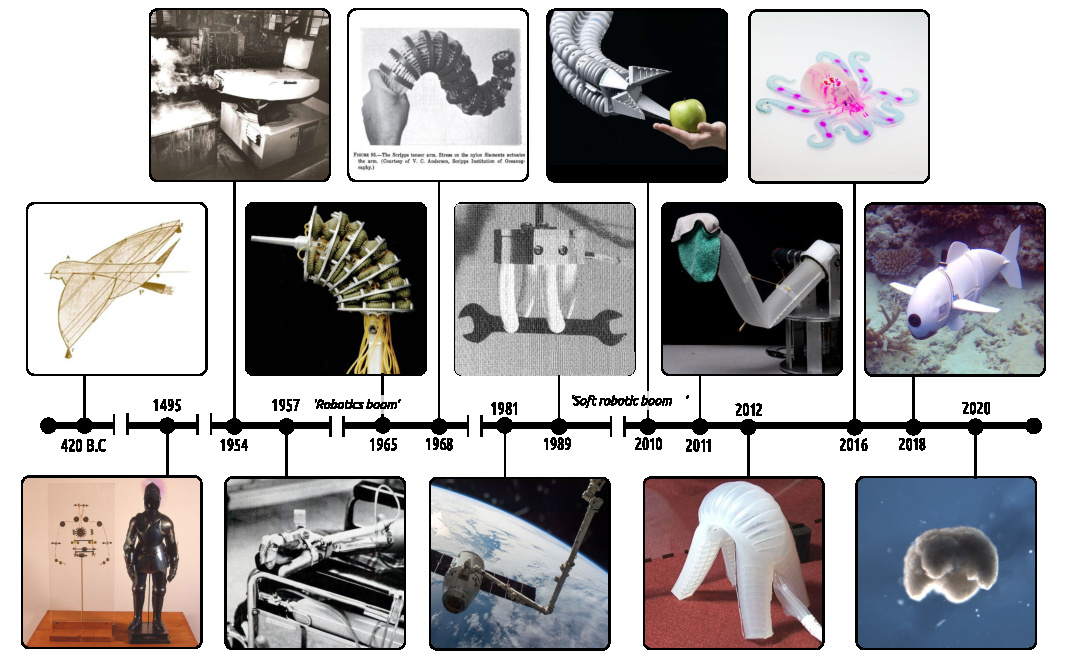
\includegraphics[width=1.11\textwidth]{./3_chapters/0_introduction/img/timeline_printer.pdf}
\fi
\caption{A brief timeline of the state-of-the-art of bio-inspired robotics throughout human history. {(1954):} Unimate, the first industrial robot . 
{(1957):} McKibben actuator, an early soft actuator inspired by the human muscle used for rehabilitation purposes \cite{Mckibben}. 
{(1965):} The Orm, believed to be the first soft robotic system designed by  Scheinman and Leifer \cite{BibEntryOrm2019Sep}. 
(1968): Tensor Scripps arm developed by Anderson \cite{Anderson1968}.
{(1981):} Canadarm-1, early flexible robotics employed on the International Space Station. 
{(1983):} Robot Arm with Pneumatic Gripper by Teleshev \cite{Teleshev1981}.
{(1984):} Bellows robotic arm by Wilson et al. \cite{Wilson2007}.
{(1989):} The soft robotic gripper developed by Suzumori et al. \cite{Suzumori1991,Suzumori1992}, seen as one of the earliest \textit{academic} soft robot, developed before the word \emph{soft robot} existed. 
{(2010):} Festo's Bionic arm inspired by the elephant's trunk \cite{Grzesiak2011}. 
{(2011):} Soft inflatable robot arm by Sanan and Atkeson \cite{Sanan2013,BibEntryBH62022Sep}.
(2012) Multi-gait soft robot capable of terrestial locomotion \cite{Choi2011}. 
(2016): Octobot, the first autonomous 3D-printed soft robot that explores a stabilizing oscillator chemical network that produces preprogrammed repetitive motion \cite{Wehner2016}.
(2018): Autonomous robotic fish made by Katzschmann \cite{Katzschmann2018}.
(2020): Xenobot, an organic soft robot composed of skin and muscle cells made by Blackiston and Kriegman \cite{Kriegman2019}.
}
\label{fig:C0:timeline}
\end{figure}
\clearpage
}

%\textbf{(Biomimicry in early automata)} One of the earliest examples of bio-mimicry is a mechanical wooden dove developed by mathematician Archytas of Tarentum in 350 BC. According to historians, the system was driven by compressed air or an internal steam-driven engine to achieve forward propulsion. It was believed to achieve traveling distances of ~200 \si{\meter} (see note\footnote{It was unclear if the devices was attached to a rope, or autonomous flight was achieved.}). Although might argue its lacks to sophistication to be considered a \emph{robot}, Archytas's invention could be considered as one of the earliest examples aviation, as its mechanical principles of achieving motion are undoubtedly similar to nowadays \emph{drone} technology. A millennium later, in the period of the High Renaissance, Leonardo da Vinci designed and constructed a mechanical knight around the 1490's -- and is thought to be the earliest robotic system. The mechanical constructions are perhaps closer to classical robots given our current perspective, and it was capable of various complex motions using preprogrammed sequences. 
%It is well-known that his work was built upon extensive anatomical research, which may have facilitated a deep understanding of the human body into the mechanical knight's robotic design. Given the work of Archytas and Da Vinci, biomimicry played a paramount role in the development of robot technologies before the term \emph{robot} was even introduced.

%\par In the 1920's, shortly after the second industrial revolution (1870 - 1914) and the first world war (1914), the first usage of the work \emph{robot} appeared -- originally meaning 'forced labor by serfs' (\ie, peasants) derived from the Czech word \emph{robota}. An common misconception is that robot implies slave, nonetheless, its origin is somewhat related. The word was popularized by Karel \v{C}apek in his play R.U.R. (Rossum’s Universal Robots) that involves an inventor named Rossum who discovers the secret of creating human-like machines. In his play, Rossom's robots assisted or fully alleviated mankind from any labor. Through human's ambition to assimilate man and machine, the robots ultimately gained the capacity for emotions. Shortly after, the robots, who were created to serve humans, have come to dominate mankind completely. The word \emph{robotics} was later solidified by Isaac Asimov, adapting the term from \v{C}apek. These works of science fiction are perhaps the fundamental groundwork of modern robotics which have led to the base practices of robotics and its corresponding academic field.

\textbf{Early soft actuation in robotics}. To relate the historical progress of soft robots to rigid robots, let us begin with early rigid robots. In 1954, George Devol filed a patent describing an autonomous robotic machine that could be preprogrammed to execute step-by-step motions \cite{Mickle2008}. The machine was designed to reduce the workload on the manufacturing work floor, with a major focus on mimicking repetitive (exhausting) human labor. In 1958, those prototypes led to a robotic system under the name \emph{Unimate}. An illustration of this early rigid robot is shown in Figure \ref{fig:C0:timeline}. The Unimate was used for manipulating metal die-casts and welding these to the main body of automobiles. In doing so revolutionizing the car industry shortly after. Much later (1969), Victor Scheinman created the Stanford Arm \cite{BibEntryStanford2022Sep,BibEntryOrm2019Sep}, recognized as the first electronic computer-controlled robotic arm because the Unimate's instructions (\ie, predefined setpoints in joint space) were prerecorded on a magnetic drum. He later developed the well-known PUMA robot in 1972 (video available at \cite{BibEntryPuma2022Sep}) -- the successor to the Unimate. Keep Scheinman in mind, as he ultimately ties to early soft robots. \vspace{0.085em}

\afterpage{
\begin{figure}[!t]
  %\hspace*{-1mm}
  \ifx\printFigures\undefined
  \else
  \centering
  %% This file was created by matlab2tikz.
%
%The latest updates can be retrieved from
%  http://www.mathworks.com/matlabcentral/fileexchange/22022-matlab2tikz-matlab2tikz
%where you can also make suggestions and rate matlab2tikz.
%
\definecolor{mycolor1}{rgb}{0.06275,0.35686,0.84706}%
\definecolor{mycolor2}{rgb}{0.86667,0.21176,0.10980}%
%
\begin{tikzpicture}

\begin{axis}[%
width=0.602\textwidth,
height=0.161\textwidth,
at={(0\textwidth,0.015\textwidth)},
scale only axis,
axis on top,
xmin=0.5,
xmax=2426.5,
tick align=outside,
y dir=reverse,
ymin=0.5,
ymax=650.5,
axis line style={draw=none},
ticks=none
]
\addplot [forget plot] graphics [xmin=0.5, xmax=2426.5, ymin=0.5, ymax=650.5] {fig_1_1-1.png};
\end{axis}

\begin{axis}[%
width=0.302\textwidth,
height=0.191\textwidth,
at={(0.648\textwidth,0\textwidth)},
scale only axis,
xmin=0,
xmax=1.5,
xlabel style={font=\color{white!15!black}},
xlabel={pressure (kPa)},
ymin=0,
ymax=35,
axis background/.style={fill=white},
xmajorgrids,
ymajorgrids,
legend style={at={(0.03,0.97)}, anchor=north west, legend columns=2, legend cell align=left, align=left, draw=white!15!black}
]
\addplot [color=mycolor1, line width=1.5pt]
  table[row sep=crcr]{%
0	0\\
0.00600149999999999	3.0568983103671\\
0.012003	5.35826739157104\\
0.024006	7.86017230302163\\
0.036009	9.05072762147565\\
0.0480119999999999	9.795136933107\\
0.0600149999999999	10.3164705929212\\
0.0720179999999999	10.711316657325\\
0.0840209999999999	11.0279129564825\\
0.0960239999999999	11.2925201532359\\
0.108027	11.5206742947192\\
0.1260315	11.8150953044601\\
0.144036	12.0694590939099\\
0.1620405	12.2959065095095\\
0.1860465	12.5672572998435\\
0.2100525	12.8138561366798\\
0.24006	13.0980192458931\\
0.276069	13.4149916949781\\
0.3180795	13.7633415653589\\
0.372093	14.1910487738014\\
0.456113999999999	14.8357726162343\\
0.588146999999999	15.8481229823956\\
0.660164999999999	16.4166289214781\\
0.726181499999999	16.9548047718235\\
0.786196499999999	17.4617841353458\\
0.840209999999999	17.9350495132933\\
0.894223499999999	18.4266813211065\\
0.948236999999999	18.9389704257632\\
0.996248999999999	19.413653689242\\
1.044261	19.9084481551956\\
1.092273	20.4253835409611\\
1.140285	20.9666992209241\\
1.1822955	21.4623032550621\\
1.224306	21.9803397018051\\
1.2663165	22.5228818415618\\
1.308327	23.0922527983715\\
1.3503375	23.6910711317645\\
1.392348	24.322306181775\\
1.43435850000001	24.9893459441392\\
1.47036750000001	25.5925254860443\\
1.4999985	26.11365092975\\
};
\addlegendentry{$\delta V$}

\addplot [color=mycolor2, line width=1.5pt]
  table[row sep=crcr]{%
0	0\\
0.00600149999999999	0.57694322540025\\
0.012003	1.8809393408942\\
0.0180045	2.95152432065056\\
0.024006	4.45583458122557\\
0.036009	6.19378149929854\\
0.0480119999999999	7.48539157943733\\
0.0600149999999999	8.4688855095399\\
0.0720179999999999	9.23690647886306\\
0.0840209999999999	9.85153659933535\\
0.0960239999999999	10.3531922792834\\
0.108027	10.7691384956111\\
0.12003	11.1184532554937\\
0.132033	11.4148904215117\\
0.144036	11.6686090629544\\
0.156039	11.8872685256996\\
0.168042	12.0767485361297\\
0.180045	12.2416363770546\\
0.192048	12.3855638977444\\
0.204051	12.511445089458\\
0.216054	12.6216464418373\\
0.228057	12.7181110468447\\
0.24006	12.8024503578201\\
0.252063	12.8760129819895\\
0.264066	12.9399369280069\\
0.276069	12.9951897701871\\
0.288072	13.0425998730449\\
0.300075	13.0828809209488\\
0.312078	13.1166513764424\\
0.324081	13.1444500557612\\
0.336084	13.1667487016037\\
0.348087	13.1839622118741\\
0.36009	13.1964570224759\\
0.372093	13.2045580243864\\
0.384096	13.2085543078992\\
0.3900975	13.2090949291082\\
};
\addlegendentry{$\delta\text{ \!\!L}$}

\addplot [color=mycolor2, dashed, line width=1.5pt, forget plot]
  table[row sep=crcr]{%
0.3900975	13.2090949291082\\
0.4021005	13.2074094834352\\
0.4141035	13.2022150575773\\
0.426106499999999	13.1937085356179\\
0.438109499999999	13.1820674082842\\
0.450112499999999	13.167452053111\\
0.462115499999999	13.1500076917316\\
0.480119999999999	13.1188216524309\\
0.498124499999999	13.0819593181423\\
0.516128999999999	13.0397643773147\\
0.534133499999999	12.9925364907466\\
0.552137999999999	12.940537547495\\
0.576143999999999	12.8641761270216\\
0.600149999999999	12.7802040746341\\
0.624155999999999	12.6890133020198\\
0.654163499999999	12.5653689878037\\
0.684170999999999	12.4314807991557\\
0.714178499999999	12.2877652488207\\
0.744185999999999	12.134547035545\\
0.780194999999999	11.9384837181762\\
0.816203999999999	11.7293863338915\\
0.852212999999999	11.5074325334682\\
0.888221999999999	11.2726938851784\\
0.924230999999999	11.0251466514001\\
0.960240000000001	10.7646794022534\\
1.0022505	10.4442081230322\\
1.044261	10.1054386868975\\
1.0862715	9.74777996411718\\
1.128282	9.3704926101939\\
1.1702925	8.97268281045118\\
1.212303	8.55329199813728\\
1.2543135	8.11108229372756\\
1.296324	7.64461717852633\\
1.3383345	7.15223665142942\\
1.380345	6.63202579865352\\
1.4223555	6.08177530074445\\
1.4583645	5.58429802632113\\
1.4943735	5.06103909220648\\
1.4999985	4.97621111560656\\
};
\end{axis}
\end{tikzpicture}%
  \fi
  \vspace{-3mm}
  \caption{Working principle of a basic pneumatic artificial muscle (\ie, Morin muscle \cite{Morin1953}) with the internal volume \data{Matlab1} in \si{\milli \liter}, and the end-effector displacement \data{Matlab2} in \si{\milli \meter} and \dashdata{Matlab2} is the point at which the undesirable ballooning occurs.
  \label{fig:C0:mckibben}}
\end{figure}

\begin{figure}[!t]
  \vspace{-0.6mm}
  \ifx\printFigures\undefined
  \else
  \centering
  %%!TEX root = ../../thesis.tex
%%%% CHAPTER 1 *****************************************************************
\chapter[Dynamic modeling of Soft Robots -- PCC case]{Dynamic modeling -- The Piece-wise Constant Approach}
\label{chap: chapter 1}

\blankfootnote{This chapter is based on:\\ .\disclaimer}

%%%% ABSTRACT ******************************************************************
%!TEX root = ../../thesis.tex
\chapterabstract{The motion complexity and use of exotic materials in soft robotics call for accurate and computationally efficient models intended for control. To reduce the gap between material and control-oriented research, we build upon the existing Piecewise-Constant Curvature framework by incorporating hyper-elastic and visco-elastic material behavior. In this work, the continuum dynamics of the soft robot are derived through the differential geometry of spatial curves, which are then related to Finite-Element data to capture the intrinsic geometric and material nonlinearities. To enable fast simulations, a reduced-order integration scheme is introduced to compute the dynamic Lagrangian matrices efficiently, which in turn allows for real-time (multi-link) models with sufficient numerical precision. By exploring the passivity and using the parametrization of the hyper-elastic model, we propose a passivity-based adaptive controller that enhances robustness towards material uncertainty and unmodeled dynamics -- slowly improving their estimates online. As a study case, a fully 3D-printed soft robot manipulator is developed, which shows good correspondence with the dynamic model under various conditions, e.g., natural oscillations, forced inputs, and under tip-loads. The solidity of the approach is demonstrated through extensive simulations, numerical benchmarks, and experimental validations.}


%%%% MAIN **********************************************************************
\section{Introduction} \label{sec: chap1 1_introduction}
%!TEX root = ../../thesis.tex
The field of soft robotics has attracted the interest of many researchers from different backgrounds. Soft robots use compliant and hyper-elastic materials, while the use of rigid materials is minimized. The introduction of soft materials into robotics greatly expanded the field of application for robotics. For example, due to their dexterity and environmental robustness, soft robots are often used in medical applications \cite{Polygerinos2015b, Yap2015, Asbeck2015}, adaptive grasping \cite{Galloway2016, Hughes2016}, and locomotion in uncertain environments \cite{Drotman2017}. Unlike its rigid counterpart, soft robots undergo large continuum-bodied motion that, to some extent, resembles morphologies found in nature. These morphologies arise by virtue of the low compliance in soft materials and, more importantly, the structural layout of the soft robot. As of today, many of the fundamental engineering principles in rigid robotics, like design, actuation, sensing, and control, are often not applicable to soft robotics systems. Since its inception, most of these engineering problems have remained challenging or unresolved.

Although the diversity in soft robotics is significant, ranging from adaptive grippers to soft manipulators, most topologies in soft robotics can be associated with nature or engineered geometries for minimal compliance (e.g., bellow shapes). Soft robots often mimic living creatures and their morphologies, e.g., the tentacle of an octopus \cite{Galloway2016, Wehner2016}, or the trunk of an elephant \cite{Drotman2017}. Hypothetically, the abundance of bio-mimicry in soft robotics might be associated with the design complexity of developing robots from soft materials. The large number of degrees-of-freedom and exotic mechanical nature of soft robots makes design significantly challenging, and consequently, the design process can be iterative and time-consuming \cite{Wehner2016}. Therefore, it becomes potentially advantageous to use computational tools that assist or develop appropriate soft robotic topologies given a set of user-defined requirements, like desired motion or force.

In the past, researchers have made efforts to finding morphologies through mathematics, in particular through evolutionary algorithms. The concept of automated creature designs was first introduced by Sims \cite{Sims1994}, who showed that, given a set of basic geometries, locomotive organisms could be generated from evolutionary algorithms. These virtual organisms resembled biological morphologies to some extent; however, the complexity of the material layout was limited. More recent work involving the synthesis of virtual soft robots includes Cheney et al. \cite{Cheney2013}, who successfully produced intricate locomotive morphologies using artificial neural networks and multi-material parameter spaces of active and passive soft voxels. Other work involving morphological synthesis includes \cite{Bern2019, Morzadec2019,Diepen2019}. Unfortunately, the synthesis of morphologies from previous approaches, though novel, remains only in ideal simulated environments. An accurate representation of the nonlinear material properties in soft robotics can be challenging, and in favor of computational efficiency, little detail is spent on the nonlinear nature governing soft materials. Besides, these evolutionary frameworks typically involve a network of `activation' cells or voxels that perform ideal volumetric deformation, biologically resembling muscle functionality while unfortunately lacking resemblance to conventional actuation in soft robotics, e.g., pneumatics, dielectrics, and smart metal alloys (SMA).

Reviewing previous methods, a more efficient approach for solving the optimal morphology might be founded in topology optimization. Topology optimization is the general formulation of a material distribution problem for mechanical solids, where density-based topologies arise throughout an iterative (non-convex) optimization procedure. The synthesis of compliant mechanisms through topology optimization is investigated thoroughly \cite{Sigmund2015, Gain2013, Luo2015}; however, its application to soft robotics is relatively unexplored \cite{Zhang2018,Zolfagharian2019}. Yet, to obtain meaningful topologies for soft robotics, two problems need to be addressed. Since soft robots undergo large deformations, it becomes necessary to describe the nonlinear geometrical deformations accurately. Inherent to significant deformation of soft materials is the importance of nonlinear material behavior, like hyperelasticity. Another concern is the design-dependency of the external forces, in our case, the pneumatic loads. This class of structural problems is more challenging than traditional problems since the load is continuously interacting with the adaptive interface during the iterative optimization process \cite{Wang2016, Vasista2013}. It should be mentioned that the use of compressed air or pressurized fluid is a popular actuation approach in soft robotics.

In this work, we present a novel framework for generating topologies of soft robotics. Contrary to biometry or convectional designs, finding the (optimal) material layout of the soft robot is accomplished through a gradient-based nonlinear topology optimization, where the distribution of soft materials is optimized given a user-defined objective. Our main contributions include the description of nonlinear geometrical deformation and pneumatic loading. We exploit the connectivity properties in polygonal meshes such that synchronized volumetric contraction or expansion of a group of polygonal elements can artificially mimic the geometrical loads in pneumatic actuation. The advantages of our framework in comparison to other literature are: ($i$) a better representation of pneumatic actuation in soft robotics; ($ii$) improved design convergence in contrast to evolution-based optimization methods. To our knowledge, our approach of pressure-driven nonlinear topology optimization is new for soft robotics, and its application could easily extend to other soft robotic systems. %The computational framework detailed in this work is made publicly available at \cite{Caasenbrood2019}.

The remainder of the paper is structured as follows. In section \ref{chap:fem}, we will discuss the continuum mechanics for hyper-elastic materials, followed by a description of the optimization scheme for soft robotics. In section \ref{chap:results}, we propose a numerical example for developing a soft robotic structure to illustrate the effectiveness of our approach.


\newpage
\section{Continuum dynamic model}  \label{sec: chap2 section header}
%!TEX root = ../../thesis.tex
As mentioned previously, soft robots are composed of soft bodies that may be regarded as a continuum body with (theoretically) infinitely many degrees-of-freedom (DOF). In this section, we aim to derive a compact and computationally efficient model that envelops the continuous dynamics of a soft robot through a small set of generalized coordinates $\q\in\Q$ and their respective generalized velocities \highlight{$\dq(t)\in T_{\q}\Q$} with $n$ the number of active joint variables. We base {the modeling framework on the work of Mochiyama et al.\cite{Mochiyama2003} who outlined a theoretical foundation for continuum manipulators. Their work is extended upon by including extensibility, serial-chaining of multiple soft-links, pneumatic actuation, and the introduction of nonlinear and time-dependent material behavior. Earlier modeling strategies addressing similar issues can be found in from Godage et al. \cite{Godage2015,Godage2016}, Della Santina et al. \cite{Santina2020,Santina2020b,Santina2020Pcc}, Renda et al. \cite{Renda2018}, and Boyer et al. \cite{Boyer2021}. Leveraging from the aforementioned works, the continuous dynamics of a soft robot manipulator can be written in the familiar Lagrangian form:
%
\begin{equation}
\MB(\q) \ddq + \vec{h}(\q,\dq) = \Qnc,
\end{equation}
%
where $\MB(\q)  \in \R^\nn$ denotes the generalized inertia matrix, $\vec{h}(\q,\dq) \in \R^n$ a vector of nonlinear state-dependent force contributions. In this work, a similar modeling framework is adopted; however, we propose an extension to incorporate FEM-driven data to more accurately reflect the underlying continuum mechanics -- in particular hyper-elasticity; and we propose a numerical scheme that allows for fast computation of the continuous dynamics. For completeness, we will recapitulate on the modeling approach here.

\subsection{Kinematics of elastic continuum bodies}
\noindent To represent the hyper-flexible configuration of the soft robot, let us consider a smooth spatial curve that passes through the geometric center of the continuously deformable body, as shown in Figure \ref{fig:configuration}. {In literature, this curve is called} the '\textit{backbone curve}' as it simplifies the three-dimensional deformation imposed by distributed forces acting on the elastic body. The arc-length of the backbone corresponds to the extensible length of the soft robot denoted by the variable $l(t) \in [l_{-},l_{+}]$ which we assume bounded $l_{+} \ge l \ge l_{-}$, and let $L$ be a constant denoting the {total unstressed} length of the soft robot. Next, let us introduce a spatial variable
$\sigma \in \Xs$ that belongs to the one-dimensional material domain of the backbone curve, i.e., $\Xs = [0,\, L]$. {Let it be clear that the spatial variable $\sigma$ represents the arc-length of a material coordinate along the undeformed material domain of the soft robot manipulator.}

\commentary{}{Figure here of smooth curve for p and Phi}

Given each material coordinate, we wish to find a suitable low-dimensional joint representation $q(t)$ such that the position vector $^0p$ anywhere on the continuous backbone can be written as a mapping from generalized coordinates and space into $\mathbb{R}^3$:
%
\begin{equation}
^0\pB: \Xs \times \Q(t) \to \R^3;
\end{equation}
%
and similarly the rotation matrix $^0\mat{\Phi}(\sigma,\vec{q})$ by a mapping from the generalized coordinates and space into $\SO{3}$:
%
\begin{equation}
^0\PhiB: \Xs \times \Q(t) \to \SO{3}, \label{eq:phi_map}
\end{equation}
%
where {$\SO{3}$ denotes the special orthogonal group for rotations about the origin of $\R^3$}, and $n = \dim(\vec{q})$ the state dimension. Under this notion, the position vectors $^0p(q,0)$ and {$^0\pB(L,\q)$} relate to the base and the end-effector of the soft robot, respectively. {Please note that left-sided superscript are used to indicate the frame of reference.} The set of all points on the backbone $\mathcal{P} = \left\{^0\pB \in \R^3\, |\, \sigma \in \Xs \right\}$ draws a possible {spatial} configuration of the soft robot given {a time instance $t \in \mathbb{T}$ on a finite horizon $\mathbb{T} = [0,T]$}.
%
\begin{intermez}
Despite the inherent flexibility in soft robotics, it is sometimes sufficient to express the kinematics according to the Piecewise Constant Curvature (PCC) condition. Mathematically, it implies that the curvature of the continuous body satisfies $\kappa(q,\sigma_1) = \kappa(q,\sigma_2)$ for a neighboring region of points $\sigma_1,\sigma_2 \subseteq \Xs$. As a result, this condition allows us to describe the full forward kinematics with a significantly reduced set of generalized coordinates, mitigating kinematic complexity in the model. Numerous works employ PCC models \cite{Falkenhahn2015,Katzschmann2019,Tatlicioglu2007,Marchese2016,Godage2016,Santina2020Pcc}, and depending on the degrees of elasticity, the PCC condition has been proven to be consistent for various soft robotic systems.
\end{intermez}
%
{Following this Piecewise Constant Curvature (PCC) description, let us assign a coordinate frame that twists minimally along the backbone -- a Bishop frame \cite{Bishop1975}-- parametrized by the following generalized coordinate vector:}
%
\begin{equation}
\vec{q} = \begin{pmatrix}
\,\varepsilon & \kappa_x & \kappa_y\,
\end{pmatrix}^\top \in \mathcal{Q},
\label{eq:coordinate}
\end{equation}
%
\noindent where {$\varepsilon \in \R$ is the elongation strain}, and $\kappa_x,\,\kappa_y\in\mathbb{R}$ are the curvatures or angular strains in $x$-$z$ and $y$-$z$ plane, respectively; and $\mathcal{Q} \subset \R^3$ is an admissible space on which $q$ evolves.It is worth mentioning that the joint description above is somewhat related to Renda. et al. \cite{Renda2018} who proposed a Piece-wise Constant Strain (PCS) parametrization with the exception of including the twist along the tangent.

By exploring the differential geometry of the smooth backbone curve similar to Mochiyama et al.\cite{Mochiyama2003}, we can express the spatial change of the position vector $^0 \vec{p}(0,\vec{q})$ and the orientation matrix $^0\mat{\Phi}(q,\sigma)$ for each material point $\sigma$ along the smooth backbone by
%
\begin{align}
\renewcommand*{\arraystretch}{2}{}
\frac{\partial \,^0\!\mat{\Phi}}{\partial \sigma}(\sigma,\vec{q}) & = \, ^0\mat{\Phi}(\sigma,\vec{q})\,\left[\mat{\Gamma} (\sigma,\vec{q}) \right]_{\times}, \label{eq:change_phi} \\
\frac{\partial \,^0\! \vec{p}}{\partial \sigma}(\sigma,\vec{q}) & = \, ^0\mat{\Phi}(\vec{q},\sigma) \, \vec{U}(\sigma,\vec{q}), \label{eq:change_p}
\end{align}
%
where $[\vec{\Gamma}]_\times \in \So{3}$ is a skew-symmetric matrix composed of the entries of the vector $\vec{\Gamma} \in \R^3$, and $\vec{U}\in \R^3$ a vector representing the tangent along the extensible backbone. The vectors $\vec{\Gamma}$ and $\vec{U}$ are vectors that define the differential geometry of the backbone, which are unique entries that lives in the tangent space of the rigid-body transformation group $\SE{3}$. Given the Bishop parametrization as described by \eqref{eq:coordinate}, these geometric entities yield
%
\begin{equation}
\vec{\Gamma} = \begin{pmatrix} -\kappa_y \\ \kappa_x \\ 0  \end{pmatrix}; \quad \quad \quad \vec{U} = \begin{pmatrix} \,\, 0 \,\, \\ \,\, 0 \,\, \\ \, \,\varepsilon \,\, \end{pmatrix} + \vec{U}_0,
\end{equation}
%
with $\vec{U}_0 = (0,0,1)^\top$ the unit-tangent. Now, given an initial configuration of backbone's base, i.e., $^0 \mat{\Phi}(0,\vec{q}) = \vec{\Phi}_0$ and $^0 \vec{p}(0,\vec{q}) = 0_3$, we can now solve for the position and orientation for each material coordinate $\sigma$ along the backbone:
%
\begin{align}
^0\mat{\Phi}(\sigma,\vec{q}) & = \vec{\Phi}_0\exp(\sigma [\vec{\Gamma}(\vec{q})]_\times), \label{eq:phi_exact} \\
^0\vec{p}(\sigma,\vec{q}) & = \int_0^\sigma\,^0\mat{\Phi}(\eta,\vec{q})\, \vec{U}(\vec{q}) \; d\eta, \label{eq:pos_vector}
\end{align}
%
where $\exp: \So{3} \to \SO{3}$ is the exponential map. Let it be clear that the closed-form solutions \eqref{eq:phi_exact} and \eqref{eq:pos_vector} form the forward configuration kinematics of the backbone curve. To express the forward velocity kinematic, let  $\vec{V}(\sigma,\vec{q},\dot{\vec{q}}) = \left(^\sigma \vec{\omega}^\top,^\sigma \vec{v}^\top \right)^\top \in \R^6 \cong \Se{3}
$ be the aggregate of the angular velocity and linear velocity components relative to an inertial frame at $\sigma$ (the frame of reference is denoted by a left superscript), where the space $\Se{3}$ denotes the Lie algebra of $\SE{3}$. The velocity twist is computed by the following integration procedure:
%
\begin{equation}
 \vec{V}(\sigma,\vec{q},\dot{\vec{q}}) = \Ad_{\mat{g}(\sigma,\cdot)}\inv \int_0^\sigma \Ad_{\mat{g}(\eta,\cdot)}\, J^*\! \dot{q}\;d\eta
 \,=:\, J(q,\sigma) \dot{q}, \label{eq:vel_cont}
\end{equation}
%
where $\Ad_g: \SE{3} \to \mathbb{R}^{6\times 6}$ denotes the adjoint transformation matrix regarding the rigid body transformation $g \in \SE{3}$ that maps local velocities (i.e., twist) to a frame located at $\sigma$, and $J^*$ a constant joint-axis matrix. The joint-axis matrix for an extensible and bendable PCC segment parametrized by the Bishop parameters is given by
%
\begin{equation}
\renewcommand*{\arraystretch}{1}{}
J^* := \left(\dfrac{\p \Gamma}{\p q}^\top \; \dfrac{\p U}{\p q}^\top \right)^\top  = \begin{pmatrix}
\,0 & 0 & 0 & 0 & 0 & 1 \, \\
\,0 & 1 & 0 & 0 & 0 & 0 \,  \\
\,-1 & 0 & 0 & 0 & 0 & 0 \,  \\
\end{pmatrix}^\top. \label{eq:joint-axis-matrix}
\end{equation}
%
Although we based the forward kinematics on the work of Mochiyama et al.\cite{Mochiyama2003}, the derived expression for the velocity twist in \eqref{eq:vel_cont} is analogous to the work of Renda et al.\cite{Renda2018,Renda2020}, and Boyer et al. \cite{Boyer2010,Boyer2021}. Please also note that \eqref{eq:vel_cont} gives rise to the geometric manipulator Jacobian $J(q,\sigma)
$ that defines the mapping from joint velocities to the velocity twist for a particular material point $\sigma$ on the continuous body. In continuation, let us also introduce the acceleration twist\cite{Boyer2021,Mochiyama2003,Renda2018} -- obtained through time differentiation of \eqref{eq:vel_cont}:
%
\begin{align}
\dot{V}(q,\dot{q},\ddot{q},\sigma) & = J \ddot{q} + \Ad_{g(\cdot,\sigma)} \inv \int_0^\sigma \Ad_{g(\cdot,\eta)}
\ad_{V(\cdot,\eta)} \, J^*\! \dot{q}\;d\eta \notag \\
& := J(q,\sigma)\ddot{q} + \dot{J}(q,\dot{q},\sigma) \dot{q},
\label{eq:acceleration}
\end{align}
%
where $\ad_{V} \in \mathbb{R}^{6\times 6}$ denotes the adjoint transformation regarding the velocity twist $V \in \Se{3}$. The reader is referred to Appendix A for more detailed expressions on the adjoint transformations.
%
\subsection{Euler-Lagrange equations}
\noindent Given the forward kinematics in \eqref{eq:phi_exact}, \eqref{eq:pos_vector}, \eqref{eq:vel_cont} and \eqref{eq:acceleration}, we can shift our attention to formulating the finite-dimensional dynamics of the soft robot. Our goal here is to write the spatio-temporal dynamics of the hyper-elastic soft robot as a second-order ODE into the Lagrangian form:
%
\begin{equation}
\frac{d}{d t}\left(\frac{\partial \mathcal{L}}{\partial \dot{{q}}}\right) - \frac{\partial \mathcal{L}}{\partial {q}} = {Q}^{\nc}, \label{eq:euler_largrange}
\end{equation}
%
\noindent where $\La({q},\dot{q}) := \T(q,\dot{q}) - \mathcal{U}(q)$ is the Lagrangian function, $\T \in \Rp$ and $\mathcal{U}\in \R$ the kinetic and potential energy, respectively; and $Q^{\nc} \in \mathbb{R}^n$ a vector of generalized non-conservative forces. To apply the Lagrangian formalism to a continuum dynamical system, regard an infinitesimal slice of the continuum body for each material coordinate $\sigma$ along the backbone curve. Given this notion, we embody this infinitesimal slice with an inertia tensor $
\mathcal{M} = \text{blkdiag}(\rho I_3,\mathcal{J_\sigma})$ with $\rho = m/L$ the line-density and $J_\sigma$ a tensor for the second moment of inertia. The kinetic energy can be obtained through spatial integration of its respective kinetic energy densities\cite{Boyer2010,Mochiyama2003,Tatlicioglu2007}, i.e., $\mathfrak{T} = \frac{1}{2}V^\top \mathcal{M} V
$:
%
\begin{align}
\mathcal{T}({q},\dot{{q}}) & = \frac{1}{2}\int_\Xs {V}({q},\dot{q},\sigma)^\top\,\mathcal{M}\,{V}({q},\dot{{q}},\sigma) \; d \sigma,
 \notag \\
& =  \frac{1}{2} \dot{q}^\top \int_\Xs  J({q},\sigma)^\top\,\mathcal{M}\, J({q},\sigma) \; d \sigma \, \dot{q}, \notag \\
& = \frac{1}{2}\dot{q}^\top M(q) \dot{q}. \label{eq:kinetic_energy}
\end{align}
%
Note that expression for the kinetic energy naturally gives rise to the generalized inertia matrix $M(q)$ of the Lagrangian model. By substitution of the kinetic energy into the Euler-Lagrange equation \eqref{eq:euler_largrange}, we find $M(q)\ddot{q} + C(q,\dot{q})q$ where $C(q,\dot{q})$ denotes the Coriolis matrix. Instead of computing the Coriolis matrix through the conventional Christoffel symbols\cite{Murray1994}, we adopt a computational scheme by Garofalo et al. \cite{Garofalo2013} used for serial-chain rigid manipulators, in which we replaced the finite summation of $N$ rigid-bodies by a spatial integration over the continuum domain $\Xs$:
%
\begin{equation}
C(q,\dot{q}) = \int_\Xs J(q,\sigma)^\top \Ct_{V(q,\dot{q},\sigma)}J(q,\sigma)\; + J(q,\sigma)^\top \Mt \dot{J}(q,\dot{q},\sigma) \; d \sigma,\label{eq:coriolis}
\end{equation}
%
where $\Ct_{V} = -\Ct_{V}^\top :=  \mathcal{M} \ad_{V}  - \ad_{V} ^\top \mathcal{M}$ is a skew-symmetric matrix. The computation above is slight different from existing literature\cite{Boyer2021,Renda2020} to ensure that the matrix $\dot{M} - 2C$ is skew-symmetric; the so-called the passivity condition\cite{Murray1994} for Euler-Lagrange systems (see Appendix B for proof). The importance of this property will become apparent later in the energy-based controller design. Lastly, the potential energy is given by sum of gravitational potential energy and internal elastic potential, i.e., $\mathcal{U}({q}) = \mathcal{U}_g({q}) + \mathcal{U}_e({q})
$. Since gravitational potential energy density is \rewritten{given} by $\mathfrak{U}_g = -\rho\,^0p(q,\sigma) \gamma_g$ with $\gamma_g \in \R^3$ is a vector of body accelerations, the potential energy related to gravity is obtained by spatial integration of their respective energy densities:
%
\begin{equation}
\mathcal{U}_g({q}) = - \rho \int_\Xs \,^0p(q,\sigma)^\top \gamma_g \; d \sigma.
\label{eq:potential_energy_grav}
\end{equation}
%
\noindent To model the hyper-elastic nature, lets introduce two nonlinear stiffness functions for both stretching and bending, denoted by $k_e: \R \mapsto \Rsp$ and $k_b: \R \mapsto \Rsp$, respectively. These functions allow us to describe a collective elastic behavior imposed by the hyper-elastic materials and the continuum-bodied deformation. It shall be clear that these entities are unique to the soft robot's geometry and soft material choice, and thus finding a suitable candidate model requires further analysis. Later, we will sculpt these nonlinear stiffness functions through Finite Element Methods (FEM). For now, we assume that these analytical nonlinear stiffness functions are known, and thus the (hyper)-elastic potential energy takes the form
%
\begin{equation}
\mathcal{U}_e({q}) = \int_0^{\varepsilon} k_e(\eta) \,\eta \; d \eta + \int_0^{\beta(q)} k_b(\eta)\, \eta \; d \eta,
\label{eq:potential_energy_elas}
\end{equation}
%
where $\varepsilon$ is the elongation strain, and $\beta({q}) = \kappa L (\varepsilon + 1)$ is the bending angle with the total curvature of the soft segment $\kappa = \sqrt{{\kappa_x}^2 + {\kappa_y}^2}$ (see Figure \ref{fig:configuration}).
\subsection*{Overall dynamics}
\noindent Finally, by combining \eqref{eq:euler_largrange}, \eqref{eq:kinetic_energy}, \eqref{eq:coriolis}, \eqref{eq:potential_energy_grav}, and \eqref{eq:potential_energy_elas}, the continuum dynamics of the soft robot can be casted into the familiar closed form \cite{Santina2020Pcc,Boyer2021,Renda2018,Godage2016} similar to aforementioned model (1):
%
\begin{align}
M({q})\,\ddot{{q}} + {C}({q},\dot{{q}})\,\dot{{q}} + P({q},\dot{q}) + G({q}) & = \tau(u,\delta), \label{eq:dynamic_model}
\end{align}
%
\noindent where $P = d \mathcal{U}_e/d q + R\dot{q}$ is a vector of generalized forces imposed by the deformation of the soft materials with $R \in \R^{n\times n}$ the Rayleigh damping matrix, $G = \p \mathcal{U}_g/\p q$ a vector of generalized gravitational forces, and $u \in \R^m$ the control input with the index $m$ the number of pressure inputs. The generalized input vector is chosen of the form: $\tau(u,\delta) = H u + \delta$ with $H: \R^m \mapsto \R^n$ a mapping from the input space to the joint actuation space, and $\delta(t)$ an external disturbance (e.g., unmodelled material uncertainties).
%
\begin{rmk}
Given the context of manipulators, a possible disturbance $\delta(t)$ could be an external mass applied to the tip of the soft robot. Given the kinematic relations in \eqref{eq:vel_cont} and \eqref{eq:acceleration}, one can describe the disturbance (modeled here as a point-mass located at $L$) by a state-dependent vector:
%
\begin{equation}
\delta_m = m_\delta \floor{J(\cdot,L)}_3^\top\left({\normalfont \Ad}_{g(\cdot,L)}\inv\gamma_g + \floor{\dot{V}(\cdot,L)}_3 \right),
\label{eq:delta_payload}
\end{equation}
%
where $\floor{\cdot}_3$ extracts the last three rows of a matrix or vector, and $m_\delta > 0$ the applied mass to the end-effector. It is worth recalling that the acceleration twist can be computed through the geometric Jacobian and its time derivative, i.e., $\dot{V} = J\ddot{q} + \dot{J}\dot{q}$. Indeed, the PCC condition for a soft body can only accurately describe the true dynamics if external forces produced by mass $m_\delta$ do not excessively exceed the intrinsic elastic balancing forces $P(q)$. Alternatively, a soft body can be modeled using multiple PCC curves of smaller size, similar to standard Finite Element discretization.
\end{rmk}

The actuation mapping $H$ depends on the geometry, placement, and orientation of the (pneumatic) soft actuators. Since the pneumatic chambers are aligned parallel to the backbone curve and are equally spaced along the circumference, we propose the following ansatz:
%
\begin{equation}
H: = \begin{pmatrix} \alpha_{\varepsilon} & \hdots & \alpha_{\varepsilon} \\ -\alpha_{\kappa} \cos(\phi_1) & \hdots & -\alpha_{\kappa} \cos(\phi_m) \\ \alpha_{\kappa} \sin(\phi_1) & \hdots & \alpha_{\kappa} \sin(\phi_m) \end{pmatrix},
\label{eq:mapping_H}
\end{equation}
%
where $\alpha_{\varepsilon},\alpha_{\kappa} > 0$ are system parameters representing the effective transferal of differential pressure to joint forces, and $\phi_i = (i-1)\cdot\tfrac{2\pi}{m}$ the angular inter-distance between the $m$-number of pneumatic bellows. Please note that the parameters $\alpha_{\varepsilon}$ and $\alpha_{\kappa}$ are dependent on the bellow area and radius from the bellow to the backbone curve.
%


\newpage
\section{Extension to multi-link dynamics}  \label{sec: chap2 section header}
%!TEX root = ../../thesis.tex
\noindent We previously expressed the position and velocity kinematics as explicit functions of the generalized coordinates (i.e., Bishop parameters) and their time-derivatives. This explicit dependency stems from the PCC conditions inferring the curvature is non-varying along the spatial domain $\Xs$, i.e., $\kappa(q,\sigma) = \kappa(q)$. Although sufficient for some cases, the condition is generally restrictive, and to some extent inconvenient, since the inclusion of multiple links demands piece-wise integration of the kinematics \eqref{eq:pos_vector}, \eqref{eq:phi_exact}, \eqref{eq:vel_cont}, and \eqref{eq:acceleration}. Rather than separation of integration, we can extend this PCC description by using piece-wise continuous spatial function to distinguishes multiple soft-bodied links along the continuous body of the soft robot. The idea of parametrization through shapes functions has been explored earlier by Chirikjian et al.\cite{Chirikjian1994,Chirikjian1992}, and later by Boyer et al. \cite{Boyer2021}, Della Santina et al. \cite{Santina2020b}. A similar discontinuous shape function series was used by Berthet-Rayne et al. \cite{Berthet2021} to pursue multi-body dynamics for growing continuum robots; and proposed by Chirikjian \cite{Chirikjian1992} for hyper-redundant robots earlier.

Following the aforementioned works, let us parameterize the the geometric vectors $\Gamma$ and $U$ for a $N$-link soft robot through the product of a basis of orthonormal functions $\!\{s_i\}_{i \in \N}$ and the Bishop parametrization as follows
%
\begin{align} \Gamma(q,\sigma) & = \sum^N_{i=1} s_i(\sigma) \ceil{J^*}_3
\,\tilde{q}_i, \label{eq:theta_extent} \\ U(q,\sigma) & = \sum^N_{i=1} s_i(\sigma)
\floor{J^*}_3\,\tilde{q}_i + U_0, \label{eq:h_extent} \end{align}
%
where $J^*$ is the joint-axis matrix as in \eqref{eq:adjoint_matrix}, the mathematical operators $\ceil{\cdot}_3$ and $\floor{\cdot}_3$  extract the first or last three rows of a matrix, respectively;  $\tilde{q}_i$ the joint variables of the $i$-th link, and $s_i: \Xs \mapsto \{0,1\}$ is a piece-wise continuous shape function, whose purpose is to be non-zero for a given interval on $\Xs$.
The new generalized coordinate vector becomes the aggregate of all joint variables of the multi-body soft robotic system $q =  \left(\tilde{q}_1^\top,\,\tilde{q}_2^\top,...,\,\tilde{q}_N^\top \right)^\top$ with the vector $\tilde{q}_i = (\varepsilon_{i},\, \kappa_{x,i},\,\kappa_{y,i})^\top$ relating to the Bishop parametrization of the $i$th-link. Given \eqref{eq:theta_extent} and \eqref{eq:h_extent}, we may now rewrite the velocity-twist as
%
\begin{equation} V(q,\dot{q},\sigma) = \Ad_g^{-1}
\int_0^\sigma \Ad_g J^* S(\sigma) \; d\sigma \dot{q} := J(q,\sigma) \dot{q}
\label{eq:vel_vec_dis} \end{equation}
%
where $S = (s_1,\,s_2,\,...,s_N) \otimes I_n$ is an unitary selection matrix derived from the basis of piece-wise continuous shape functions $\!\{s_i\}_{i=1}^N$. To be less ambiguous about this selection matrix $S$, lets consider a spatial coordinate $\sigma_2 \in [L_1,L_1+L_2]$ that lies on the spatial interval of the second link. Consequently, the operation $S(\sigma_2) {q} = {\tilde{q}}_2$ returns the corresponding joint variable of the second link. This selection of
generalized coordinates follows analogously for other links along the serial-chain of the soft manipulator. We provided a small library of piece-wise continuous shape functions upto $1 \le N \le 8$ links under \texttt{./src/pwf} on the open repository\cite{Caasenbrood2021}.
Now, substitution of the discontinuous variation of the geometric Jacobian in \eqref{eq:vel_vec_dis} into \eqref{eq:kinetic_energy} leads to the dynamic model of a $N$-link soft robot manipulator in the
Lagrangian form similar to \eqref{eq:dynamic_model}.


\section{Efficient solver of the soft robotic dynamics through Matrix-Differential Equations}  \label{sec: chap2 section header}
%!TEX root = ../../thesis.tex
Due to the partial differential nature of soft robots, obtaining a closed-form expression for the projected Lagrangian model in \eqref{eq:dynamic_model} can become notoriously long and complex (especially for multi-link systems). The origin of this problem stems from the integrands of inertia matrix $M(q)$ in \eqref{eq:kinetic_energy} and Coriolis forces $C(q,\dot{q})$ in \eqref{eq:coriolis}; which become highly nonlinear and therefore difficult to calculate a-priori. As a result, solving the forward dynamics using traditional solvers often deteriorates the real-time performance, and in turn its usability for closed-loop control. Inspired by Boyer et al. \cite{Boyer2021} and Godage et al \cite{Godage2016}, instead of finding an exact solution to the dynamic entries $M(q)$, $C(q,\dot{q})$ and $G(q)$, let us introduce a similar reduced-order integration scheme that produces an approximate of the dynamic model \eqref{eq:dynamic_model}. Yet, instead of using an inverse Newton-Euler algorithm (i.e., Featherstone or Hollerbach scheme) in which the Lagrangian entries are built column-wise, we propose an explicit integration scheme that efficiently computes all Lagrangian entities in parallel through a so-called Matrix-Differential Equation (MDE).

The idea here is to replace all necessary spatial integrations for the computation of the Lagrangian entities by an equivalent Matrix-Differential Equation of the form:
%
\begin{equation}
\frac{\p Z}{\p \sigma} = F(Z,\sigma), \label{eq:MDE}
\end{equation}
%
where $Z(\cdot,\sigma)$ is a matrix-valued function composed of the necessary elements for the forward kinematics and forward dynamics, and $F(Z,\sigma)$ a matrix-valued flow function that describes the spatial evolution of $Z$. Then, by choosing the appropriate initial condition for $Z(\cdot,0) = Z_0$ and numerically solving \eqref{eq:MDE} over a finite horizon $\Xs$, we can retrieve an approximate of the Lagrangian model in \eqref{eq:dynamic_model} by extracting the necessary elements from the solution $Z(\cdot,L)$.

Before describing the MDE, let us first introduce two intermediate matrices related to the computation of the manipulator Jacobian and its time-derivative, namely:
%
\begin{align}
\frac{\p B_1}{\p \sigma} & = \Ad_{g(\cdot,\sigma)}\, J^* S(\sigma), \\
\frac{\p B_2}{\p \sigma} & = \Ad_{g(\cdot,\sigma)}\ad_{V(\cdot,\sigma)}\, J^* S(\sigma)
\end{align}
%
such that they satisfy $J\dot{q} = \Ad_g\inv B_1 \dot{q}$ and $ \dot{J} \dot{q} = \Ad_g\inv B_2 \dot{q}$. Given the expressions above, we can now include a partial computation Jacobians into the MDE. By collecting all the differential relation for the forward kinematics (5), (6) and forward dynamics (14), (15), and (16), we can assign a flow function $F:= \text{blkdiag}\left(F_1,F_2 \right)$ composed of two matrices:
%
\begin{align}
F_1 & = \begin{pmatrix}
\begin{matrix}
^0 \Phi [\Gamma]_\times & ^0 \Phi U \\ 0_{3\times3} & 0_3
\end{matrix} \, \vrule & \Ad_g J^*S &\vrule\;\; \Ad_g \ad_{V} J^* S
 \end{pmatrix}, \\
F_2 & = \begin{pmatrix}
\frac{\p M}{\p \sigma} & \frac{\p C}{\p \sigma} & \frac{\p G}{\p \sigma}  \end{pmatrix},
\end{align}
%s
in which the differential form of the dynamic entities $M(q)$, $C(q,\dot{q})$, and $G(q)$ of the Lagrangian model are given by
%
\begin{align}
\frac{\p M}{\p \sigma} & = (\Ad_{g}\inv B_1)^\top \mathcal{M} (\Ad_{g}\inv B_1), \\[0.4em]
\frac{\p C}{\p \sigma} & = (\Ad_{g}\inv B_1)^\top \left[\mathcal{C}_V (\Ad_{g}\inv B_1) + \mathcal{M} (\Ad_{g}\inv B_2) \right], \\[0.4em]
\tfrac{\p G}{\p \sigma} & = (\floor{B_{1}}_3)^\top \rho \gamma_g,
\end{align}
%
We wish to stress that $F_1$ collects all elements related to the forward kinematics, whereas $F_2$ contains the dynamic entities related to the Lagrangian model. Following the spatial Matrix-Differential equation in \eqref{eq:MDE} above, its solution will be a matrix $Z := \text{blkdiag}\left( Z_1,Z_2 \right)$ composed of two smaller state matrices $Z_1$ and $Z_2$:
%
\begin{align}
Z_1 & := \begin{pmatrix}
\begin{matrix}
^0 \Phi  & ^0 p \\ 0_{3\times3} &  0_{3}
\end{matrix} \;\; \vrule & \!B_1 & \vrule & \!B_2 \;\;\;
 \end{pmatrix}, \\
Z_2 & := \begin{pmatrix} M & C & G \end{pmatrix},
\end{align}
%
Such a Matrix-Differential equation as in \eqref{eq:MDE} are not supported natively by standard ODE solvers. Therefore, an explicit second-order Runge-Kutta solver for MDEs is developed such that efficiently computes the evolution of the state matrix $Z$ along $\Xs$. The solver is written in \texttt{MATLAB} and can be found under \texttt{./src/Model.m} at Caasenbrood \cite{Caasenbrood2020}.

As for state trajectories along the temporal regime $\mathbb{T} = [0,T]$, an implicit trapezoidal integration scheme is proposed to solve the approximated continuum dynamics, which are generally less conservative on discretization to preserve numerical stability. Here implicit schemes are favored over explicit scheme, since a coarser time integration can significantly increase real-time performance. In addition, to further boost performance of the temporal integration, a cost-effective approximation of the Hessian is introduced. For more detail, see Appendix C for more detail.


%%%%%%%%%%%%%%%%%%%%%%%%%%%%%%%%%%%%%%%%%%%%%%%%%%%%%%%%%%%%%%%%%%%%%%%%%%%%%%%%

  %\input{/home/brandon/Documents/phd/thesis/3_chapters/0_introduction/img/PAM.pdf_tex}
  \fi
  \caption{Patent diagrams of pneumatic artificial muscle from 1953 till 1988. (a) Morin Muscle (1953, \cite{Morin1953}); (b) ROMAN muscle (1986, \cite{Immega1986}); (c) Yarlott muscle (1972, \cite{Yarlott1972}); (d) Kukolj muscle (1988, \cite{Kukolj1988}); (e) Paynter Hyperboloid (1974, \cite{Paynter1974}).
  \label{fig:C0:several_PAM}}
  \vspace{-5mm}
\end{figure}
}

Nearly four years after the Unimate was developed, Joseph L. McKibben developed a pneumatic muscle-inspired actuator capable of linear contraction -- called the McKibben actuator. The McKibben muscle is a type of Pneumatic Artificial Muscle (PAM) which is to this date the most frequently used and published artificial muscle in literature. According to \cite{Mckibben}, he developed the McKibben actuators to bring motion to his little daughter's polio-paralyzed hand. His aim was that eventually such pneumatic actuators may help patients with paralyzed fingers to move, grasp, and even write. Inspired by the human muscle, the McKibben actuator consists of an inflatable inner bladder enveloped with a double-helical weave. When pressurized, the fluidic actuator converts radial expansion into uni-axial contraction \cite{Daerden1999,Daerden2000,Schulte1961} since weave inhibits extensive \emph{ballooning} -- a term for undesired rapidly-accelerated volumetric expansion. Its material composition is often silicone rubber with a nylon-fiber exterior. A schematic representation of a general pneumatic muscle and the effect of ballooning are shown in Figure \ref{fig:C0:mckibben}. Ballooning is an (often undesired) nonlinear effect, where the hyper-elastic pressure vessel exhibits strain-softening after a critical point is reached. As a result, further increase of the pressure leads to an exponential growth in volume, which ultimately leads to actuator tearing. At stages of ballooning, mechanical performance significantly drops and even produces adverse effects, like actuation reversal. McKibben solved this problem through a combination of soft and inextensible fiber weaves. These inextensible were placed at the exterior wall of the soft muscle, thereby limiting the radial expansion before ballooning could occur. According to Daerden (1999, \cite{Daerden1999}), there exist many variations of pneumatic muscle besides braided muscles, such as the \emph{netted muscles} (e.g, Yarlott \cite{Yarlott1972}, ROMAC \cite{Immega1986}, and Kukolj \cite{Kukolj1988}) and \emph{embedded muscles} (\eg, Morin \cite{Morin1953}, Paynter Hyperboloid \cite{Paynter1988}). Illustration of their patent schematics are shown in Figure \ref{fig:C0:several_PAM}.

Pneumatic muscles are perhaps one of the first fundamental technologies that enabled soft robotics, and to this day, it remains a framework for many soft robotic systems. Nevertheless, besides the many examples of fluidics \cite{Marchese2014,Marchese2016,Katzschmann2018,Suzumori1991,Mosadegh2014}, there exist many other technologies employed in soft robotic motion: such as thermal \cite{Wu2021Dec} or chemical expansion/contraction \cite{Tolley2014,Bartlett2015,Wehner2016}, crystal re-alignment \cite{Pilz2020,Lopez2018,Vantomme2021,Polygerinos2013}, di-electric elastomers \cite{Keplinger2011}, magnetism \cite{Roh2019Apr,KimYoonho2018,McDonald2020,Boyvat2017Jul}, and naturally the use of tendons paired with electro-mechanical actuation \cite{Renda2018,Bern2019,Kim2020Jun,Coevoet2017Feb,Wang2016Sep}. Some predate the invention of the McKibben actuator. For example, a popular soft actuation principle still applied in soft robotics today are Dielectric Elastomer Actuators (DEA) developed by R\"{o}ntgen in 1880 \cite{Rontgen1880}. Therefore, given the abundance of soft robotic actuation, it is difficult to pinpoint the exact date of origin of soft actuation technology. Note, however, that these systems are not categorized as soft robots, they are categorized as soft actuators. Here, we emphasize the difference between soft actuators and soft robots in view of the modeling and control terminology relevant to the thesis:

\terminology{\textbf{Soft actuators} are controllable flexible actuation units of the constitute soft robot that through external stimuli are responsible for natural motion and/or change in adaptive compliance. %By definition, a soft actuator is a single-input-multi-output (SIMO) system.
}{}
%
\vspace{-4mm}
%
\begin{rmk} The terminology above attempts to address an ambiguity common to soft robotics, namely the interchangeable use of soft actuator and soft robot. The thesis invokes that soft robots must be comprised of multiple soft actuators that connect to a passive deformable body. Here, the soft body functions as a mechanical conduit between actuators, sensors, and the environment.
\end{rmk}
  %Let us also introduce the dual of soft actuators -- namely the \emph{soft sensor} that relate measurements to the motion of soft actuators:

\textbf{Origin of soft robotics}. Returning to 1965, nearly a decade after the invention of the McKibben actuator and the Unimate robot, Scheinman and Leifer proposed a novel pneumatic robotic arm named the \emph{Orm} -- Norwegian for snake (recall that he also developed the popular PUMA robot \cite{BibEntryPuma2022Sep}). The name was also an abbreviation for Object-Relational Mapping tool \cite{Corke2020}. To the author's knowledge, this is believed to be the first instance of a soft robotic system. Surprisingly the system predates any rigid snake-like robot, like the Scripps tensor arm by Anderson (1968, \cite{Anderson1968}). Inspired by the anatomy of snakes, the system featured 28 rubber pneumatic artificial muscle (\ie, bellows) distributed along a flexible backbone (\ie, skeletal support). The network of artificial muscles were sandwiched between steel plates to prevent misalignment. It is worth mentioning that the technology is analogous to the pneumatic McKibben muscle, where fiber weaves are used to prevent ballooning. Yet, contrary to a single McKibben actuator, the soft robotic system could undergo three-dimensional movement by inflation or deflation of an embedded pneumatic network. This led to a rich set of movements previously unseen in rigid robotics. As an illustrative example, we provided the mechanics of the Orm soft robot in Figure \ref{fig:C0:ormrobot}. The soft robot could achieve bending in any preferred direction by differential pressurization of each channel, and elongation through synchronized actuation. Most notably, comparing the volume-strain response of the Orm with respect to the McKibben actuator, \ie, comparing Figure \ref{fig:C0:mckibben} against \ref{fig:C0:ormrobot}, it is noticeably more linear in nature. Although not documented at the time, the comparison highlights the importance of structural geometry in pneumatic muscle networks.

\begin{figure}[!t]
  \ifx\printFigures\undefined
  \else
  \centering
  %% This file was created by matlab2tikz.
%
%The latest updates can be retrieved from
%  http://www.mathworks.com/matlabcentral/fileexchange/22022-matlab2tikz-matlab2tikz
%where you can also make suggestions and rate matlab2tikz.
%
\definecolor{mycolor1}{rgb}{0.06275,0.35686,0.84706}%
\definecolor{mycolor2}{rgb}{0.86667,0.21176,0.10980}%
%
\begin{tikzpicture}

\begin{axis}[%
width=0.583\textwidth,
height=0.214\textwidth,
at={(0\textwidth,0\textwidth)},
scale only axis,
axis on top,
xmin=0.5,
xmax=1768.5,
tick align=outside,
y dir=reverse,
ymin=0.5,
ymax=650.5,
axis line style={draw=none},
ticks=none
]
\addplot [forget plot] graphics [xmin=0.5, xmax=1768.5, ymin=0.5, ymax=650.5] {fig_orm_elong-1.png};
\end{axis}

\begin{axis}[%
width=0.308\textwidth,
height=0.195\textwidth,
at={(0.642\textwidth,0.01\textwidth)},
scale only axis,
xmin=0,
xmax=15,
ymin=0,
ymax=110,
axis background/.style={fill=white},
xmajorgrids,
ymajorgrids,
legend style={at={(0.03,0.97)}, anchor=north west, legend columns=2, legend cell align=left, align=left, draw=white!15!black}
]
\addplot [color=mycolor1, line width=1.5pt]
  table[row sep=crcr]{%
0	0\\
1.20005999999999	8.62875869322605\\
2.40012	17.0685830193392\\
3.60017999999999	25.3075020924564\\
4.80024	33.3362750448029\\
6.0003	41.1480614223673\\
7.20036	48.7381311097239\\
8.40042	56.1036109498542\\
9.60048	63.2432605846741\\
10.80054	70.1572704477627\\
11.700585	75.1955238137271\\
12.60063	80.1081200969719\\
13.500675	84.8973166125783\\
14.40072	89.5642639584667\\
15.00075	92.6047602820568\\
};
\addlegendentry{$\delta V$}

\addplot [color=mycolor2, line width=1.5pt]
  table[row sep=crcr]{%
0	0\\
1.500075	9.4713120804718\\
3.00015	18.7367798341987\\
4.20021	25.9889383302985\\
5.40027000000001	33.0912743243296\\
6.60033	40.0387557751286\\
7.80039000000001	46.8277828635893\\
9.00045	53.4559850403998\\
10.20051	59.922055247927\\
11.40057	66.2256106025044\\
12.60063	72.3665219327312\\
13.80069	78.346840194486\\
15.00075	84.1642843326511\\
};
\addlegendentry{$\delta L$}

\end{axis}

\begin{axis}[%
width=1.08\textwidth,
height=0.244\textwidth,
at={(-0.022\textwidth,-0.015\textwidth)},
scale only axis,
xmin=0,
xmax=1,
ymin=0,
ymax=1,
axis line style={draw=none},
ticks=none,
axis x line*=bottom,
axis y line*=left
]
\end{axis}
\end{tikzpicture}%
  %% This file was created by matlab2tikz.
%
%The latest updates can be retrieved from
%  http://www.mathworks.com/matlabcentral/fileexchange/22022-matlab2tikz-matlab2tikz
%where you can also make suggestions and rate matlab2tikz.
%
\definecolor{mycolor1}{rgb}{0.06275,0.35686,0.84706}%
\definecolor{mycolor2}{rgb}{1.0000,0.6157,0.1176}%
%
\begin{tikzpicture}

\begin{axis}[%
width=0.583\textwidth,
height=0.186\textwidth,
at={(0\textwidth,0.005\textwidth)},
scale only axis,
axis on top,
xmin=0.5,
xmax=2037.5,
tick align=outside,
y dir=reverse,
ymin=0.5,
ymax=650.5,
axis line style={draw=none},
ticks=none
]
\addplot [forget plot] graphics [xmin=0.5, xmax=2037.5, ymin=0.5, ymax=650.5] {./fig/fig_orm_bend-1.png};
\end{axis}

\begin{axis}[%
width=0.308\textwidth,
height=0.195\textwidth,
at={(0.642\textwidth,0\textwidth)},
scale only axis,
xmin=0,
xmax=30,
xlabel style={font=\color{white!15!black}},
xlabel={pressure (kPa)},
ymin=0,
ymax=110,
axis background/.style={fill=white},
xmajorgrids,
ymajorgrids,
legend style={at={(0.03,0.97)}, anchor=north west, legend columns=2, legend cell align=left, align=left, draw=white!15!black}
]
\addplot [color=mycolor1, line width=1.5pt]
  table[row sep=crcr]{%
0	0\\
1.60008	2.43048322137711\\
4.0002	6.19782561266756\\
4.80024	7.46829805994749\\
5.60028	8.34214292028537\\
17.60088	25.9279210387424\\
18.40092	27.0804871808147\\
19.20096	27.8807159907824\\
20.001	29.291815814346\\
20.80104	30.1255987953186\\
21.60108	31.5485305130109\\
22.40112	32.3659198775631\\
24.0012	34.5026095847334\\
28.80144	41.0337024135815\\
30.40152	43.1793137664006\\
};
\addlegendentry{$\delta V$}

\addplot [color=mycolor2, line width=1.5pt]
  table[row sep=crcr]{%
0	0\\
3.20016	8.88556718870406\\
6.40032000000001	17.5260854409956\\
8.80043999999999	23.7584681055126\\
11.20056	29.7734109354827\\
13.60068	35.566935673684\\
16.0008	41.1374336291155\\
17.60088	44.7277626743178\\
20.001	50.0250200383298\\
20.80104	51.6388516477443\\
21.60108	53.3837573512613\\
22.40112	54.9453731417261\\
23.20116	56.644891426995\\
24.80124	59.8364150546849\\
26.40132	62.9180842306127\\
28.0014	65.909936141282\\
29.60148	68.8150689926074\\
30.40152	70.2358435840924\\
};
\addlegendentry{$\theta$}

\end{axis}

\begin{axis}[%
width=1.08\textwidth,
height=0.244\textwidth,
at={(-0.022\textwidth,-0.024\textwidth)},
scale only axis,
xmin=0,
xmax=1,
ymin=0,
ymax=1,
axis line style={draw=none},
ticks=none,
axis x line*=bottom,
axis y line*=left
]
\end{axis}
\end{tikzpicture}%
  \vspace{-6mm}
  \fi
  
  \caption{Working principle of the Orm robotic manipulator \cite{BibEntryOrm2019Sep} with the internal volume \data{Matlab1} in \si{\milli \liter}, and the end-effector displacement \data{Matlab2} in \si{\milli \meter} and bending-angle \data{Matlab4} in deg. By actuation of the pneumatic network, both elongation and bending can be achieved. Observe that the response is significantly more linear than McKibben actuators in Fig. \ref{fig:C0:mckibben}, emphasizing the importance of geometry.
  %\dotdata{Matlab2}
  \vspace{-6mm}
  \label{fig:C0:ormrobot}}
\end{figure}

According to an interview with Scheinman led by Asaro et al. \cite{ETHW2020Dec} in 2010, the positional accuracy of the system was poor, yet the concepts of pneumatically-driven soft arms continued for many years. The positional inaccuracy of pneumatic soft actuators at the time may have caused its lost of academic interest in the 60's. Three years later, in 1968, an improved hyper-redundant robot manipulator was proposed and patented by Anderson and Horn \cite{Anderson1968} (see Figure \ref{fig:C0:timeline}). Improving upon the Orm, which was deemed slow and had limited positional accuracy, Anderson proposed an array of nylon tendons that were connected to rigid discs distributed along the redundant backbone of the robot. The configurable backbone was comprised of universal spherical joints that allow for pivoting motion with respect to other discs -- totalling 16 Degrees-of-Freedom (DOFs). The entire arm was actuated hydraulically, yet the (soft) actuators were placed outside the robot's body rather than placed at each joint, like the Orm. To improve positional accuracy further, Anderson placed sensor tendons parallel the actuator tendons which allowed for operator-based positional feedback. Although Anderson's robot does not categorize as a soft robot since it relies mostly on rigid materials, its flexibility arose from thin nylon tendons that were used for both actuation and sensing. Anderson showed that a network of distributed sensors are necessary to control the complex morphological shapes in  hyper-redundant robotic systems, while also mitigating the sensor's effect on mobility. Within this context, let us define soft sensors:

\terminology{\textbf{(Proprioceptive) soft sensors} are flexible measurements units embedded into the soft robotic body that through external stimuli measure the (local) changes of the system. Softness here implies that the sensor minimally alters the global mechanical behavior of the robot. %By definition, a soft sensor is a multi-input-single-output (MISO) system.
}{}
%
\begin{rmk}
  \vspace{-1mm}
As the emphasize lies on "minimally alters the global mechanical behavior", soft sensors may be composed of stiff (perhaps even rigid) components. Our definition infers that these sensors must be placed into or onto the soft body, minimally affecting the operational workspace of the soft actuator network in static or dynamic condition.
\end{rmk}

\textbf{Soft robotics in the 80's}. Following the fundamental works of McKibben, Scheinman and Anderson, the field of soft Pneumatic Artificial Muscles (PAMs) in robotics evolved rapidly in the early 80's. A few soft robotic systems are shown in Figure \ref{fig:C0:earlyPAMrobots}. Teleshev (1981, \cite{Teleshev1981}) developed a soft gripper reminiscent of modern PneuNet actuators \cite{Galloway2016,Mosadegh2014,Choi2011} -- a rectangular bellow-shaped soft actuator. Unlike uniaxial PAMs, which are radially symmetric, these soft grippers explored an asymmetrical design of bellows. The geometry led to a stiffness differential around the circumference, resulting in their icon bending motion. Still popular today, these pneumatic bending actuators find their origin back in early 1974, see Andorf et al. (1974, \cite{Andorf1974}). A decade later, Takagi et al. (\cite{Takagi1983}, 1983) developed a soft multi-joint robot manipulator that resembles the human arm with its movements and antagonistic muscle pairs. Although, their PAMs -- called \textit{Rubbertuator} -- had a function and design identical to McKibben's PAMs, their system showed the merits of combining soft and rigid. They observed not only a high-degree of positional control of the robot arm, force control was easily regulated by the pressure control. This naturally had safety benefits. The soft robot arm could perform delicate low-force tasks while simultaneously blocking motion when encountering a human. These (soft) properties were lacking in rigid robotic manipulators at the time but reminiscent in its biological counterpart -- the human arm. Note that, at that time, force and impedance control for rigid robotics had been topics of academic research for years \cite{Anderson1988,Khatib1987,Hogan1984,Hogan1984Jan}, dating back to the early 1970's. (\eg, see also \cite{Markiewicz1973}). Yet achieving similar properties without control were rarely explored at the time.
%
\begin{figure}[!t]
  \vspace{-2mm}
  \ifx\printFigures\undefined
  \else
  \hspace{1mm}
  % This file was created by matlab2tikz.
%
%The latest updates can be retrieved from
%  http://www.mathworks.com/matlabcentral/fileexchange/22022-matlab2tikz-matlab2tikz
%where you can also make suggestions and rate matlab2tikz.
%
\begin{tikzpicture}

\begin{axis}[%
width=0.95\textwidth,
height=0.238\textwidth,
at={(0\textwidth,0\textwidth)},
scale only axis,
axis on top,
clip=false,
xmin=0.5,
xmax=2593.5,
tick align=outside,
y dir=reverse,
ymin=0.5,
ymax=650.5,
axis line style={draw=none},
ticks=none,
axis x line*=bottom,
axis y line*=left
]
\addplot [forget plot] graphics [xmin=0.5, xmax=2593.5, ymin=0.5, ymax=650.5] {./fig/fig_earlyPAMrobots-1.png};
\node[right, align=left]
at (axis cs:203,780) {\small (a)};
\node[right, align=left]
at (axis cs:777.5,780) {\small (b)};
\node[right, align=left]
at (axis cs:1326,780) {\small (c)};
\node[right, align=left]
at (axis cs:1801,780) {\small (d)};
\node[right, align=left]
at (axis cs:2226,780) {\small (e)};
\end{axis}
\end{tikzpicture}%
  \fi
  %\vspace{-2mm}
  \caption{Early robotic systems that explored soft PAMs for various tasks. (a) Soft robotic grippers by Teleshev (1981, \cite{Teleshev1981}). (b) The soft arm using \textit{Rubbertuator} actuators by Takagi and Sakaguchi (1983, \cite{Takagi1983}). (c) Three-link soft robotic manipulator with gripper reminiscent of the elephant's trunk, developed by Wilson at Duke University (1984, \cite{Wilson2007,Weisburd1988}). (d) Shadow bipedal walker by Buckley et al. (1988, \cite{Buckley2012}) using McKibben muscle in antagonistic pairs to produce locomotion.
  \label{fig:C0:earlyPAMrobots}}
  \vspace{-2mm}
\end{figure}
%
\par Shortly after, Wilson (1984, \cite{Wilson2007}) developed a soft robot manipulator based on the elephant's trunk at Duke University, Durham. His design effectively combined the works of Teleshev \cite{Teleshev1981} and Takagi et al. \cite{Takagi1983} into a robot with similar dexterity but minimal use of rigid components. According to \cite{Weisburd1988}, his idea stemmed from the work of Kier and Smith (1985, \cite{Kier1985}) who studied the biomechanics of muscular-hydrostats in animals, like cephalopods (\eg, squids). The work of Kier et al. \cite{Kier1985} studied how complex motions are produces in muscular organs, like elongation, shortening, bending and torsion. Inspired by the muscular hydrostat in the elephant's trunk, Wilson developed a soft arm composed of polyurethane tubes that work as half-bellows, which enabled expansion and bending under positive pressurization \cite{Weisburd1988}. To accommodate for three-dimensional movement, each soft pneumatic link was placed at a $ \phi = \frac{\pi}{2}$ twist offset w.r.t. to the previous link. To illustrate the motion of the soft arm, a few snapshots are provided in Figure \ref{fig:C0:fist_srm_robot}. Wilson hypothesized that these highly-complaint robots will be more mechanically robust and be sufficiently dexterous for tight workspaces, contrary to its rigid counterparts. Although the dexterity was novel, the positional accuracy was poor. The main problem stemmed from the soft arm being controlled in open-loop (\ie, remote tele-operation) without proprioceptive sensing nor any positional feedback control. An issue akin to the Orm (1965). 

A few years later, Buckley et al. (1988, \cite{Buckley2012}) developed the Shadow walker -- a bipedal rigid robot comprised of antagonistic McKibben muscle pairs. Although not fully soft, their system did explore proprioceptive sensing. The hip, knee, and ankle joints were equipped with resistance-variable potentiometers for position feedback, whereas all the muscles had tension sensors for force feedback. Later on, these resistive sensors were replaced by analog optical sensors to improve robustness \cite{Buckley2012}. Although the system was top-heavy, due to the pneumatic control hardware (\eg, valves and piping), rudimentary locomotion was possible. Interestingly, a similar artificial muscle system is still explored in nowadays humanoid robotics, like the Atlas from Boston Dynamics. The success of pairing soft muscles with proprioceptive sensing eventually led to the development of the McKibben Shadow hand \cite{Buckley2012,Gong2022Feb}, comprised of 40 uniquely addressable soft muscles. 

\begin{figure}[!t]
  \vspace{-2mm}
  \ifx\printFigures\undefined
  \else
  \centering
  % This file was created by matlab2tikz.
%
%The latest updates can be retrieved from
%  http://www.mathworks.com/matlabcentral/fileexchange/22022-matlab2tikz-matlab2tikz
%where you can also make suggestions and rate matlab2tikz.
%
\begin{tikzpicture}

\begin{axis}[%
width=0.712\textwidth,
height=0.295\textwidth,
at={(0.11\textwidth,0.03\textwidth)},
scale only axis,
xmin=0,
xmax=1,
ymin=0,
ymax=1,
axis line style={draw=none},
ticks=none,
axis x line*=bottom,
axis y line*=left
]
\end{axis}

\begin{axis}[%
width=0.218\textwidth,
height=0.164\textwidth,
at={(0\textwidth,0.179\textwidth)},
scale only axis,
axis on top,
xmin=0.5,
xmax=480.5,
tick align=outside,
y dir=reverse,
ymin=0.5,
ymax=360.5,
axis line style={draw=none},
ticks=none
]
\addplot [forget plot] graphics [xmin=0.5, xmax=480.5, ymin=0.5, ymax=360.5] {fig_first_srm-1.png};
\node[right, align=left, font=\color{white}]
at (axis cs:15,320) {\scriptsize $t = 0$ s};
\end{axis}

\begin{axis}[%
width=0.218\textwidth,
height=0.164\textwidth,
at={(0.227\textwidth,0.179\textwidth)},
scale only axis,
axis on top,
xmin=0.5,
xmax=480.5,
tick align=outside,
y dir=reverse,
ymin=0.5,
ymax=360.5,
axis line style={draw=none},
ticks=none
]
\addplot [forget plot] graphics [xmin=0.5, xmax=480.5, ymin=0.5, ymax=360.5] {fig_first_srm-2.png};
\node[right, align=left, font=\color{white}]
at (axis cs:15,320) {\scriptsize $t = 1.9$ s};
\end{axis}

\begin{axis}[%
width=0.218\textwidth,
height=0.164\textwidth,
at={(0.455\textwidth,0.179\textwidth)},
scale only axis,
axis on top,
xmin=0.5,
xmax=480.5,
tick align=outside,
y dir=reverse,
ymin=0.5,
ymax=360.5,
axis line style={draw=none},
ticks=none
]
\addplot [forget plot] graphics [xmin=0.5, xmax=480.5, ymin=0.5, ymax=360.5] {fig_first_srm-3.png};
\node[right, align=left, font=\color{white}]
at (axis cs:15,320) {\scriptsize $t = 2.8$ s};
\end{axis}

\begin{axis}[%
width=0.218\textwidth,
height=0.164\textwidth,
at={(0.682\textwidth,0.179\textwidth)},
scale only axis,
axis on top,
xmin=0.5,
xmax=480.5,
tick align=outside,
y dir=reverse,
ymin=0.5,
ymax=360.5,
axis line style={draw=none},
ticks=none
]
\addplot [forget plot] graphics [xmin=0.5, xmax=480.5, ymin=0.5, ymax=360.5] {fig_first_srm-4.png};
\node[right, align=left, font=\color{white}]
at (axis cs:15,320) {\scriptsize $t = 5.6$ s};
\end{axis}

\begin{axis}[%
width=0.218\textwidth,
height=0.164\textwidth,
at={(0\textwidth,0\textwidth)},
scale only axis,
axis on top,
xmin=0.5,
xmax=480.5,
tick align=outside,
y dir=reverse,
ymin=0.5,
ymax=360.5,
axis line style={draw=none},
ticks=none
]
\addplot [forget plot] graphics [xmin=0.5, xmax=480.5, ymin=0.5, ymax=360.5] {fig_first_srm-5.png};
\node[right, align=left, font=\color{white}]
at (axis cs:15,320) {\scriptsize $t = 6.5$ s};
\end{axis}

\begin{axis}[%
width=0.218\textwidth,
height=0.164\textwidth,
at={(0.227\textwidth,0\textwidth)},
scale only axis,
axis on top,
xmin=0.5,
xmax=480.5,
tick align=outside,
y dir=reverse,
ymin=0.5,
ymax=360.5,
axis line style={draw=none},
ticks=none
]
\addplot [forget plot] graphics [xmin=0.5, xmax=480.5, ymin=0.5, ymax=360.5] {fig_first_srm-6.png};
\node[right, align=left, font=\color{white}]
at (axis cs:15,320) {\scriptsize $t = 9.3$ s};
\end{axis}

\begin{axis}[%
width=0.218\textwidth,
height=0.164\textwidth,
at={(0.455\textwidth,0\textwidth)},
scale only axis,
axis on top,
xmin=0.5,
xmax=480.5,
tick align=outside,
y dir=reverse,
ymin=0.5,
ymax=360.5,
axis line style={draw=none},
ticks=none
]
\addplot [forget plot] graphics [xmin=0.5, xmax=480.5, ymin=0.5, ymax=360.5] {fig_first_srm-7.png};
\node[right, align=left, font=\color{white}]
at (axis cs:15,320) {\scriptsize $t = 10$ s};
\end{axis}

\begin{axis}[%
width=0.218\textwidth,
height=0.164\textwidth,
at={(0.682\textwidth,0\textwidth)},
scale only axis,
axis on top,
xmin=0.5,
xmax=480.5,
tick align=outside,
y dir=reverse,
ymin=0.5,
ymax=360.5,
axis line style={draw=none},
ticks=none
]
\addplot [forget plot] graphics [xmin=0.5, xmax=480.5, ymin=0.5, ymax=360.5] {fig_first_srm-8.png};
\node[right, align=left, font=\color{white}]
at (axis cs:15,320) {\scriptsize $t = 14$ s};
\end{axis}
\end{tikzpicture}%
  \fi
  %\vspace{-2mm}
  \caption{Three-link soft robotic manipulator with two-fingered soft gripper by James Wilson from Stanford university (1984, \cite{Wilson2007}). Unlike classic manipulators, where links and joints are separated, Wilson's robot consisted of three pneumatic bending actuators -- being link and joint simultaneously. 
  \vspace{-4mm}
  \label{fig:C0:fist_srm_robot}}
\end{figure}

\begin{figure}[!t]
  \vspace{-3mm}
  \ifx\printFigures\undefined
  \else
  \centering
  % This file was created by matlab2tikz.
%
%The latest updates can be retrieved from
%  http://www.mathworks.com/matlabcentral/fileexchange/22022-matlab2tikz-matlab2tikz
%where you can also make suggestions and rate matlab2tikz.
%
\begin{tikzpicture}

\begin{axis}[%
width=0.712\textwidth,
height=0.295\textwidth,
at={(0.11\textwidth,0.032\textwidth)},
scale only axis,
xmin=0,
xmax=1,
ymin=0,
ymax=1,
axis line style={draw=none},
ticks=none,
axis x line*=bottom,
axis y line*=left
]
\end{axis}

\begin{axis}[%
width=0.218\textwidth,
height=0.168\textwidth,
at={(0\textwidth,0.179\textwidth)},
scale only axis,
axis on top,
xmin=0.5,
xmax=302.5,
tick align=outside,
y dir=reverse,
ymin=0.5,
ymax=233.5,
axis line style={draw=none},
ticks=none
]
\addplot [forget plot] graphics [xmin=0.5, xmax=302.5, ymin=0.5, ymax=233.5] {fig_first_gripper-1.png};
\node[right, align=left, font=\color{white}]
at (axis cs:7,209) {\scriptsize $t = 0$ s};
\end{axis}

\begin{axis}[%
width=0.218\textwidth,
height=0.168\textwidth,
at={(0.227\textwidth,0.179\textwidth)},
scale only axis,
axis on top,
xmin=0.5,
xmax=302.5,
tick align=outside,
y dir=reverse,
ymin=0.5,
ymax=233.5,
axis line style={draw=none},
ticks=none
]
\addplot [forget plot] graphics [xmin=0.5, xmax=302.5, ymin=0.5, ymax=233.5] {fig_first_gripper-2.png};
\node[right, align=left, font=\color{white}]
at (axis cs:7,209) {\scriptsize $t = 0.14$ s};
\end{axis}

\begin{axis}[%
width=0.218\textwidth,
height=0.168\textwidth,
at={(0.455\textwidth,0.179\textwidth)},
scale only axis,
axis on top,
xmin=0.5,
xmax=302.5,
tick align=outside,
y dir=reverse,
ymin=0.5,
ymax=233.5,
axis line style={draw=none},
ticks=none
]
\addplot [forget plot] graphics [xmin=0.5, xmax=302.5, ymin=0.5, ymax=233.5] {fig_first_gripper-3.png};
\node[right, align=left, font=\color{white}]
at (axis cs:7,209) {\scriptsize $t = 0.28$ s};
\end{axis}

\begin{axis}[%
width=0.218\textwidth,
height=0.168\textwidth,
at={(0.682\textwidth,0.179\textwidth)},
scale only axis,
axis on top,
xmin=0.5,
xmax=302.5,
tick align=outside,
y dir=reverse,
ymin=0.5,
ymax=233.5,
axis line style={draw=none},
ticks=none
]
\addplot [forget plot] graphics [xmin=0.5, xmax=302.5, ymin=0.5, ymax=233.5] {fig_first_gripper-4.png};
\node[right, align=left, font=\color{white}]
at (axis cs:7,209) {\scriptsize $t = 0.55$ s};
\end{axis}

\begin{axis}[%
width=0.218\textwidth,
height=0.168\textwidth,
at={(0\textwidth,0\textwidth)},
scale only axis,
axis on top,
xmin=0.5,
xmax=302.5,
tick align=outside,
y dir=reverse,
ymin=0.5,
ymax=233.5,
axis line style={draw=none},
ticks=none
]
\addplot [forget plot] graphics [xmin=0.5, xmax=302.5, ymin=0.5, ymax=233.5] {fig_first_gripper-5.png};
\node[right, align=left, font=\color{white}]
at (axis cs:7,209) {\scriptsize $t = 0.69$ s};
\end{axis}

\begin{axis}[%
width=0.218\textwidth,
height=0.168\textwidth,
at={(0.227\textwidth,0\textwidth)},
scale only axis,
axis on top,
xmin=0.5,
xmax=302.5,
tick align=outside,
y dir=reverse,
ymin=0.5,
ymax=233.5,
axis line style={draw=none},
ticks=none
]
\addplot [forget plot] graphics [xmin=0.5, xmax=302.5, ymin=0.5, ymax=233.5] {fig_first_gripper-6.png};
\node[right, align=left, font=\color{white}]
at (axis cs:7,209) {\scriptsize $t = 0.83$ s};
\end{axis}

\begin{axis}[%
width=0.218\textwidth,
height=0.168\textwidth,
at={(0.455\textwidth,0\textwidth)},
scale only axis,
axis on top,
xmin=0.5,
xmax=302.5,
tick align=outside,
y dir=reverse,
ymin=0.5,
ymax=233.5,
axis line style={draw=none},
ticks=none
]
\addplot [forget plot] graphics [xmin=0.5, xmax=302.5, ymin=0.5, ymax=233.5] {fig_first_gripper-7.png};
\node[right, align=left, font=\color{white}]
at (axis cs:7,209) {\scriptsize $t = 0.97$ s};
\end{axis}

\begin{axis}[%
width=0.218\textwidth,
height=0.168\textwidth,
at={(0.682\textwidth,0\textwidth)},
scale only axis,
axis on top,
xmin=0.5,
xmax=302.5,
tick align=outside,
y dir=reverse,
ymin=0.5,
ymax=233.5,
axis line style={draw=none},
ticks=none
]
\addplot [forget plot] graphics [xmin=0.5, xmax=302.5, ymin=0.5, ymax=233.5] {fig_first_gripper-8.png};
\node[right, align=left, font=\color{white}]
at (axis cs:7,209) {\scriptsize $t = 1.2$ s};
\end{axis}
\end{tikzpicture}%
  \fi
  %\vspace{-2mm}
  \caption{Four-fingered soft robotic gripper by Suzumori and Saiko (1989, \cite{Suzumori1991,Suzumori1992}). Each finger possess three pneumatic chambers that allow for directional bending -- analogous the Orm. Through proper coordination of the set of soft fingers various gripping complexity can be achieved, such as the clock-wise turning a mechanical hex bolt (as shown above). Suzumori et al. showed these intricate finger motions can be easily achieved by careful modeling of the fingertip dynamics, and exploring the adaptability of soft materials.
  \label{fig:C0:fist_grip_robot}}
  \vspace{-3mm}
\end{figure}

Following, Suzumori and Saiko (1989, \cite{Suzumori1991,Suzumori1992}) developed a micro flexible soft actuator driven by an electro-hydraulic system (intrinsic length $L \approx12$ \si{\milli \meter}). Each end-effector enables three DOFs including pitch, yaw, and stretch -- making it ideal for fingers, arms and legs. Figure \ref{fig:C0:fist_grip_robot} shows the level of dexterity in their system. By placing the four PAMs parallel on a gripper mount, and assigning a pre-defined trajectory, they showed their soft robotic system has sufficient dexterity to mount an hex-bolt at an incredible speed and precision. To achieve such dexterity and precision, Suzumori et al. \cite{Suzumori1991} employed various modeling and control strategies to account for the dynamical characteristics under high-frequency, fluid compressibility, and the closing mechanics of pressure valves. Futhermore, the kinematics of each finger was derived using generalized homogenous transformation, not unlike traditional robotics. Knowing both the compliance characteristics (pressure-deformation relations) and the forward kinematics, a Jacobian-based positional controller was employed to regulate the Cartesian coordinates of the finger-tips (successfully one might add).
%
\par \textbf{Early controllers for hyper-redundant (soft) robots}. Following the increasing interest in highly-flexible robots around the late 80's, academic research into controlling these \textit{hyper-redundant} robots boomed shortly after. At the time, the term hyper-redundancy -- being an extension to redundancy in robotics \cite{MerriamWebster1983} -- was defined as the relative degree of kinematic and/or actuator redundancy which is large or even infinite \cite{Chirikjian1992,Chirikjian1994}. The term was first introduced by Chirikjian and Burdick (1989, \cite{Chirikjian1989}). Others referred to these robots as \textit{highly redundant} \cite{Wilson1988Dec,Naccarato1989Dec} or \textit{High Degree-of-Freedom} (HDOF) manipulator \cite{Salerno1989Jan,Mochiyama1999}. Around that time, Chirikjian and Burdick provided a plenary of mathematical foundation \cite{Chirikjian1994,Chirikjian1994Jun,Chirikjian1991,Chirikjian1992,Chirikjian1992Dec} focussed on the kinematics and motion planning of hyper-redundant manipulators. Their work presented a modal discretization approach to describe the shape of the deformable backbone \cite{Chirikjian1994Jun}, and from this geometric approaches were introduced to solve obstacle avoiding trajectories using generalized \textit{follow-the-leader} strategies \cite{Chirikjian1992Dec}. Especially the latter showed the limitation in rigid redundant manipulators. Although Chirikjian laid the foundation for the control of hyper-redundant robot, basic principles of motion planning in pneumatic hyper-redundant robots were already presented by Wilson et al. (1988, \cite{Wilson1988Dec,Wilson1989Jun}) -- yet were not called hyper-redundant robots nor soft robots yet. Recall also that the work of Wilson et al. has been sown earlier in Figure \ref{fig:C0:timeline} and Figure \ref{fig:C0:fist_srm_robot}. In Brock et al. (1991, \cite{Brock1991}), a similar analysis was used for optimal shape design of thin elastic rods to realize desired robotic compliance. Besides, there exist an abundance of literature prior to \cite{Chirikjian1992} on Variable Geometry Truss Manipulators (VGTMs) -- a variant of hyper-redundant tensegrity robotics -- that dealt with motion planning for such systems \cite{Naccarato1989Dec,Naccarato1991Apr,Salerno1989Jan}. Later, Mochiyama et al. \cite{Mochiyama1998,Mochiyama1999}, built upon Chirikjian's work by extending it to a dynamic formulation for elastic rods such that classic controller design is possible. They proposed shape-regulation controllers for HDOF manipulator by projecting them onto time-invariant curves, thereby showing that the estimation the desired curve parameters is the crucial key to solving the problem by Lyapunov design \cite{Mochiyama1998}. Although there existed a variety of modeling and control strategies, computational power in relation to modeling complexity was the limiting factor for the simulation-to-reality transfer at the time.

%\subsection{REF}
% \begin{itemize}
%   \item . F. Shulte, "The Characteristics of the Mckibben Artificial Muscle", The Application of External Power in Prosthetics and Orthetics, pp. 94-115, 1960.
%   \item A. Chen, R. Yin, L. Cao, C. Yuan, H. K. Ding and W. J. Zhang, "Soft robotics: Definition and research issues," 2017 24th International Conference on Mechatronics and Machine Vision in Practice (M2VIP), 2017, pp. 366-370, doi: 10.1109/M2VIP.2017.8267170.

\vspace{-4mm}
\section{Challenges in modern soft robotics}
\label{sec:C0:1.2}
%
\begin{figure}[!t]
  \vspace{-2mm}
  \ifx\printFigures\undefined
  \else
  \centering
  \vspace{-2mm}
  % This file was created by matlab2tikz.
%
%The latest updates can be retrieved from
%  http://www.mathworks.com/matlabcentral/fileexchange/22022-matlab2tikz-matlab2tikz
%where you can also make suggestions and rate matlab2tikz.
%
\definecolor{mycolor1}{rgb}{0.06275,0.35686,0.84706}%
\definecolor{mycolor2}{rgb}{0.86667,0.21176,0.10980}%
\definecolor{mycolor3}{rgb}{0.18039,0.52157,0.25098}%
\definecolor{mycolor4}{rgb}{1.00000,0.30980,0.00000}%
%
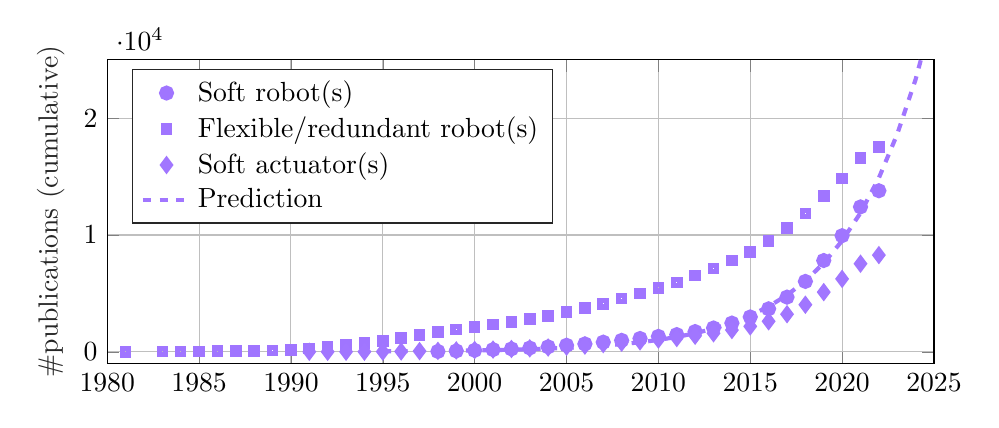
\begin{tikzpicture}

\begin{axis}[%
width=0.866\textwidth,
height=0.318\textwidth,
at={(0\textwidth,0\textwidth)},
scale only axis,
xmin=723181,
xmax=739618,
xtick={723181,725008,726834,728660,730486,732313,734139,735965,737791,739618},
xticklabels={{1980},{1985},{1990},{1995},{2000},{2005},{2010},{2015},{2020},{2025}},
scaled x ticks=false,
ymin=-1000,
ymax=25000,
ylabel style={font=\color{white!15!black}},
ylabel={\#publications (cumulative)},
axis background/.style={fill=white},
xmajorgrids,
ymajorgrids,
legend style={at={(0.03,0.97)}, anchor=north west, legend cell align=left, align=left, draw=white!15!black}
]
\addplot [color=mycolor1, line width=2.0pt, only marks, mark size=1.7pt, mark=*, mark options={solid, mycolor1}]
  table[row sep=crcr]{%
729756	31\\
730121	75\\
730486	125\\
730852	187\\
731217	247\\
731582	327\\
731947	425\\
732313	557\\
732678	675\\
733043	825\\
733408	980\\
733774	1140\\
734139	1318\\
734504	1471\\
734869	1732\\
735235	2039\\
735600	2458\\
735965	2984\\
736330	3680\\
736696	4681\\
737061	6027\\
737426	7816\\
737791	9942\\
738157	12408\\
738522	13791\\
};
\addlegendentry{Soft robot(s)}

\addplot [color=mycolor2, line width=2.0pt, only marks, mark size=1.1pt, mark=square, mark options={solid, mycolor2}]
  table[row sep=crcr]{%
723547	4\\
724277	12\\
724642	19\\
725008	34\\
725373	43\\
725738	58\\
726103	66\\
726469	117\\
726834	168\\
727199	275\\
727564	423\\
727930	582\\
728295	737\\
728660	899\\
729025	1163\\
729391	1423\\
729756	1714\\
730121	1907\\
730486	2109\\
730852	2343\\
731217	2563\\
731582	2818\\
731947	3084\\
732313	3390\\
732678	3741\\
733043	4116\\
733408	4557\\
733774	5007\\
734139	5482\\
734504	5936\\
734869	6529\\
735235	7133\\
735600	7826\\
735965	8563\\
736330	9482\\
736696	10586\\
737061	11827\\
737426	13342\\
737791	14847\\
738157	16584\\
738522	17555\\
};
\addlegendentry{Flexible/redundant robot(s)}

\addplot [color=mycolor3, line width=2.0pt, only marks, mark size=1.7pt, mark=diamond, mark options={solid, mycolor3}]
  table[row sep=crcr]{%
727199	1\\
727564	2\\
727930	4\\
728295	9\\
728660	12\\
729025	28\\
729391	55\\
729756	81\\
730121	118\\
730486	153\\
730852	190\\
731217	240\\
731582	294\\
731947	365\\
732313	439\\
732678	533\\
733043	662\\
733408	783\\
733774	894\\
734139	1050\\
734504	1179\\
734869	1375\\
735235	1584\\
735600	1864\\
735965	2175\\
736330	2612\\
736696	3218\\
737061	4031\\
737426	5109\\
737791	6243\\
738157	7542\\
738522	8281\\
};
\addlegendentry{Soft actuator(s)}

\addplot [color=mycolor4, dashed, line width=1.5pt]
  table[row sep=crcr]{%
728660	44.6634216554798\\
728660	44.6634216554798\\
728660	44.6634216554798\\
728660	44.6634216554798\\
728660	44.6634216554798\\
728660	44.6634216554798\\
728660	44.6634216554798\\
728660	44.6634216554798\\
728660	44.6634216554798\\
728660	44.6634216554798\\
728660	44.6634216554798\\
728660	44.6634216554798\\
728660	44.6634216554798\\
728660	44.6634216554798\\
728660	44.6634216554798\\
728660	44.6634216554798\\
728660	44.6634216554798\\
729025	53.3890888278004\\
729025	53.3890888278004\\
729025	53.3890888278004\\
729025	53.3890888278004\\
729025	53.3890888278004\\
729025	53.3890888278004\\
729025	53.3890888278004\\
729025	53.3890888278004\\
729025	53.3890888278004\\
729025	53.3890888278004\\
729025	53.3890888278004\\
729025	53.3890888278004\\
729025	53.3890888278004\\
729025	53.3890888278004\\
729025	53.3890888278004\\
729025	53.3890888278004\\
729025	53.3890888278004\\
729025	53.3890888278004\\
729025	53.3890888278004\\
729025	53.3890888278004\\
729025	53.3890888278004\\
729025	53.3890888278004\\
729025	53.3890888278004\\
729025	53.3890888278004\\
729025	53.3890888278004\\
729025	53.3890888278004\\
729025	53.3890888278004\\
729025	53.3890888278004\\
729025	53.3890888278004\\
729025	53.3890888278004\\
729025	53.3890888278004\\
729025	53.3890888278004\\
729025	53.3890888278004\\
729391	64.3112289380452\\
729391	64.3112289380452\\
729391	64.3112289380452\\
729391	64.3112289380452\\
729391	64.3112289380452\\
729391	64.3112289380452\\
729391	64.3112289380452\\
729391	64.3112289380452\\
729391	64.3112289380452\\
729391	64.3112289380452\\
729391	64.3112289380452\\
729391	64.3112289380452\\
729391	64.3112289380452\\
729391	64.3112289380452\\
729391	64.3112289380452\\
729391	64.3112289380452\\
729391	64.3112289380452\\
729391	64.3112289380452\\
729391	64.3112289380452\\
729391	64.3112289380452\\
729391	64.3112289380452\\
729391	64.3112289380452\\
729391	64.3112289380452\\
729391	64.3112289380452\\
729391	64.3112289380452\\
729391	64.3112289380452\\
729391	64.3112289380452\\
729391	64.3112289380452\\
729391	64.3112289380452\\
729391	64.3112289380452\\
729391	64.3112289380452\\
729391	64.3112289380452\\
729391	64.3112289380452\\
729391	64.3112289380452\\
729756	77.9827502362947\\
729756	77.9827502362947\\
729756	77.9827502362947\\
729756	77.9827502362947\\
729756	77.9827502362947\\
729756	77.9827502362947\\
729756	77.9827502362947\\
729756	77.9827502362947\\
729756	77.9827502362947\\
729756	77.9827502362947\\
729756	77.9827502362947\\
729756	77.9827502362947\\
729756	77.9827502362947\\
729756	77.9827502362947\\
729756	77.9827502362947\\
729756	77.9827502362947\\
729756	77.9827502362947\\
729756	77.9827502362947\\
729756	77.9827502362947\\
729756	77.9827502362947\\
729756	77.9827502362947\\
729756	77.9827502362947\\
729756	77.9827502362947\\
729756	77.9827502362947\\
729756	77.9827502362947\\
729756	77.9827502362947\\
729756	77.9827502362947\\
729756	77.9827502362947\\
729756	77.9827502362947\\
729756	77.9827502362947\\
729756	77.9827502362947\\
729756	77.9827502362947\\
729756	77.9827502362947\\
730121	95.095742078724\\
730121	95.095742078724\\
730121	95.095742078724\\
730121	95.095742078724\\
730121	95.095742078724\\
730121	95.095742078724\\
730121	95.095742078724\\
730121	95.095742078724\\
730121	95.095742078724\\
730121	95.095742078724\\
730121	95.095742078724\\
730121	95.095742078724\\
730121	95.095742078724\\
730121	95.095742078724\\
730121	95.095742078724\\
730121	95.095742078724\\
730121	95.095742078724\\
730121	95.095742078724\\
730121	95.095742078724\\
730121	95.095742078724\\
730121	95.095742078724\\
730121	95.095742078724\\
730121	95.095742078724\\
730121	95.095742078724\\
730121	95.095742078724\\
730121	95.095742078724\\
730121	95.095742078724\\
730121	95.095742078724\\
730121	95.095742078724\\
730121	95.095742078724\\
730121	95.095742078724\\
730121	95.095742078724\\
730121	95.095742078724\\
730486	116.516510361223\\
730486	116.516510361223\\
730486	116.516510361223\\
730486	116.516510361223\\
730486	116.516510361223\\
730486	116.516510361223\\
730486	116.516510361223\\
730486	116.516510361223\\
730486	116.516510361223\\
730486	116.516510361223\\
730486	116.516510361223\\
730486	116.516510361223\\
730486	116.516510361223\\
730486	116.516510361223\\
730486	116.516510361223\\
730486	116.516510361223\\
730486	116.516510361223\\
730486	116.516510361223\\
730486	116.516510361223\\
730486	116.516510361223\\
730486	116.516510361223\\
730486	116.516510361223\\
730486	116.516510361223\\
730486	116.516510361223\\
730486	116.516510361223\\
730486	116.516510361223\\
730486	116.516510361223\\
730486	116.516510361223\\
730486	116.516510361223\\
730486	116.516510361223\\
730486	116.516510361223\\
730486	116.516510361223\\
730486	116.516510361223\\
730486	116.516510361223\\
730852	143.329432265087\\
730852	143.329432265087\\
730852	143.329432265087\\
730852	143.329432265087\\
730852	143.329432265087\\
730852	143.329432265087\\
730852	143.329432265087\\
730852	143.329432265087\\
730852	143.329432265087\\
730852	143.329432265087\\
730852	143.329432265087\\
730852	143.329432265087\\
730852	143.329432265087\\
730852	143.329432265087\\
730852	143.329432265087\\
730852	143.329432265087\\
730852	143.329432265087\\
730852	143.329432265087\\
730852	143.329432265087\\
730852	143.329432265087\\
730852	143.329432265087\\
730852	143.329432265087\\
730852	143.329432265087\\
730852	143.329432265087\\
730852	143.329432265087\\
730852	143.329432265087\\
730852	143.329432265087\\
730852	143.329432265087\\
730852	143.329432265087\\
730852	143.329432265087\\
730852	143.329432265087\\
730852	143.329432265087\\
730852	143.329432265087\\
731217	176.891850360523\\
731217	176.891850360523\\
731217	176.891850360523\\
731217	176.891850360523\\
731217	176.891850360523\\
731217	176.891850360523\\
731217	176.891850360523\\
731217	176.891850360523\\
731217	176.891850360523\\
731217	176.891850360523\\
731217	176.891850360523\\
731217	176.891850360523\\
731217	176.891850360523\\
731217	176.891850360523\\
731217	176.891850360523\\
731217	176.891850360523\\
731217	176.891850360523\\
731217	176.891850360523\\
731217	176.891850360523\\
731217	176.891850360523\\
731217	176.891850360523\\
731217	176.891850360523\\
731217	176.891850360523\\
731217	176.891850360523\\
731217	176.891850360523\\
731217	176.891850360523\\
731217	176.891850360523\\
731217	176.891850360523\\
731217	176.891850360523\\
731217	176.891850360523\\
731217	176.891850360523\\
731217	176.891850360523\\
731217	176.891850360523\\
731582	218.902784955852\\
731582	218.902784955852\\
731582	218.902784955852\\
731582	218.902784955852\\
731582	218.902784955852\\
731582	218.902784955852\\
731582	218.902784955852\\
731582	218.902784955852\\
731582	218.902784955852\\
731582	218.902784955852\\
731582	218.902784955852\\
731582	218.902784955852\\
731582	218.902784955852\\
731582	218.902784955852\\
731582	218.902784955852\\
731582	218.902784955852\\
731582	218.902784955852\\
731582	218.902784955852\\
731582	218.902784955852\\
731582	218.902784955852\\
731582	218.902784955852\\
731582	218.902784955852\\
731582	218.902784955852\\
731582	218.902784955852\\
731582	218.902784955852\\
731582	218.902784955852\\
731582	218.902784955852\\
731582	218.902784955852\\
731582	218.902784955852\\
731582	218.902784955852\\
731582	218.902784955852\\
731582	218.902784955852\\
731582	218.902784955852\\
731582	218.902784955852\\
731947	271.48894309721\\
731947	271.48894309721\\
731947	271.48894309721\\
731947	271.48894309721\\
731947	271.48894309721\\
731947	271.48894309721\\
731947	271.48894309721\\
731947	271.48894309721\\
731947	271.48894309721\\
731947	271.48894309721\\
731947	271.48894309721\\
731947	271.48894309721\\
731947	271.48894309721\\
731947	271.48894309721\\
731947	271.48894309721\\
731947	271.48894309721\\
731947	271.48894309721\\
731947	271.48894309721\\
731947	271.48894309721\\
731947	271.48894309721\\
731947	271.48894309721\\
731947	271.48894309721\\
731947	271.48894309721\\
731947	271.48894309721\\
731947	271.48894309721\\
731947	271.48894309721\\
731947	271.48894309721\\
731947	271.48894309721\\
731947	271.48894309721\\
731947	271.48894309721\\
731947	271.48894309721\\
731947	271.48894309721\\
731947	271.48894309721\\
732313	337.312378226773\\
732313	337.312378226773\\
732313	337.312378226773\\
732313	337.312378226773\\
732313	337.312378226773\\
732313	337.312378226773\\
732313	337.312378226773\\
732313	337.312378226773\\
732313	337.312378226773\\
732313	337.312378226773\\
732313	337.312378226773\\
732313	337.312378226773\\
732313	337.312378226773\\
732313	337.312378226773\\
732313	337.312378226773\\
732313	337.312378226773\\
732313	337.312378226773\\
732313	337.312378226773\\
732313	337.312378226773\\
732313	337.312378226773\\
732313	337.312378226773\\
732313	337.312378226773\\
732313	337.312378226773\\
732313	337.312378226773\\
732313	337.312378226773\\
732313	337.312378226773\\
732313	337.312378226773\\
732313	337.312378226773\\
732313	337.312378226773\\
732313	337.312378226773\\
732313	337.312378226773\\
732313	337.312378226773\\
732313	337.312378226773\\
732678	419.705250522346\\
732678	419.705250522346\\
732678	419.705250522346\\
732678	419.705250522346\\
732678	419.705250522346\\
732678	419.705250522346\\
732678	419.705250522346\\
732678	419.705250522346\\
732678	419.705250522346\\
732678	419.705250522346\\
732678	419.705250522346\\
732678	419.705250522346\\
732678	419.705250522346\\
732678	419.705250522346\\
732678	419.705250522346\\
732678	419.705250522346\\
732678	419.705250522346\\
732678	419.705250522346\\
732678	419.705250522346\\
732678	419.705250522346\\
732678	419.705250522346\\
732678	419.705250522346\\
732678	419.705250522346\\
732678	419.705250522346\\
732678	419.705250522346\\
732678	419.705250522346\\
732678	419.705250522346\\
732678	419.705250522346\\
732678	419.705250522346\\
732678	419.705250522346\\
732678	419.705250522346\\
732678	419.705250522346\\
732678	419.705250522346\\
733043	522.838509850919\\
733043	522.838509850919\\
733043	522.838509850919\\
733043	522.838509850919\\
733043	522.838509850919\\
733043	522.838509850919\\
733043	522.838509850919\\
733043	522.838509850919\\
733043	522.838509850919\\
733043	522.838509850919\\
733043	522.838509850919\\
733043	522.838509850919\\
733043	522.838509850919\\
733043	522.838509850919\\
733043	522.838509850919\\
733043	522.838509850919\\
733043	522.838509850919\\
733043	522.838509850919\\
733043	522.838509850919\\
733043	522.838509850919\\
733043	522.838509850919\\
733043	522.838509850919\\
733043	522.838509850919\\
733043	522.838509850919\\
733043	522.838509850919\\
733043	522.838509850919\\
733043	522.838509850919\\
733043	522.838509850919\\
733043	522.838509850919\\
733043	522.838509850919\\
733043	522.838509850919\\
733043	522.838509850919\\
733043	522.838509850919\\
733043	522.838509850919\\
733408	651.933040523155\\
733408	651.933040523155\\
733408	651.933040523155\\
733408	651.933040523155\\
733408	651.933040523155\\
733408	651.933040523155\\
733408	651.933040523155\\
733408	651.933040523155\\
733408	651.933040523155\\
733408	651.933040523155\\
733408	651.933040523155\\
733408	651.933040523155\\
733408	651.933040523155\\
733408	651.933040523155\\
733408	651.933040523155\\
733408	651.933040523155\\
733408	651.933040523155\\
733408	651.933040523155\\
733408	651.933040523155\\
733408	651.933040523155\\
733408	651.933040523155\\
733408	651.933040523155\\
733408	651.933040523155\\
733408	651.933040523155\\
733408	651.933040523155\\
733408	651.933040523155\\
733408	651.933040523155\\
733408	651.933040523155\\
733408	651.933040523155\\
733408	651.933040523155\\
733408	651.933040523155\\
733408	651.933040523155\\
733408	651.933040523155\\
733774	813.523956566939\\
733774	813.523956566939\\
733774	813.523956566939\\
733774	813.523956566939\\
733774	813.523956566939\\
733774	813.523956566939\\
733774	813.523956566939\\
733774	813.523956566939\\
733774	813.523956566939\\
733774	813.523956566939\\
733774	813.523956566939\\
733774	813.523956566939\\
733774	813.523956566939\\
733774	813.523956566939\\
733774	813.523956566939\\
733774	813.523956566939\\
733774	813.523956566939\\
733774	813.523956566939\\
733774	813.523956566939\\
733774	813.523956566939\\
733774	813.523956566939\\
733774	813.523956566939\\
733774	813.523956566939\\
733774	813.523956566939\\
733774	813.523956566939\\
733774	813.523956566939\\
733774	813.523956566939\\
733774	813.523956566939\\
733774	813.523956566939\\
733774	813.523956566939\\
733774	813.523956566939\\
733774	813.523956566939\\
733774	813.523956566939\\
734139	1015.79142686097\\
734139	1015.79142686097\\
734139	1015.79142686097\\
734139	1015.79142686097\\
734139	1015.79142686097\\
734139	1015.79142686097\\
734139	1015.79142686097\\
734139	1015.79142686097\\
734139	1015.79142686097\\
734139	1015.79142686097\\
734139	1015.79142686097\\
734139	1015.79142686097\\
734139	1015.79142686097\\
734139	1015.79142686097\\
734139	1015.79142686097\\
734139	1015.79142686097\\
734139	1015.79142686097\\
734139	1015.79142686097\\
734139	1015.79142686097\\
734139	1015.79142686097\\
734139	1015.79142686097\\
734139	1015.79142686097\\
734139	1015.79142686097\\
734139	1015.79142686097\\
734139	1015.79142686097\\
734139	1015.79142686097\\
734139	1015.79142686097\\
734139	1015.79142686097\\
734139	1015.79142686097\\
734139	1015.79142686097\\
734139	1015.79142686097\\
734139	1015.79142686097\\
734139	1015.79142686097\\
734139	1015.79142686097\\
734504	1268.97477739086\\
734504	1268.97477739086\\
734504	1268.97477739086\\
734504	1268.97477739086\\
734504	1268.97477739086\\
734504	1268.97477739086\\
734504	1268.97477739086\\
734504	1268.97477739086\\
734504	1268.97477739086\\
734504	1268.97477739086\\
734504	1268.97477739086\\
734504	1268.97477739086\\
734504	1268.97477739086\\
734504	1268.97477739086\\
734504	1268.97477739086\\
734504	1268.97477739086\\
734504	1268.97477739086\\
734504	1268.97477739086\\
734504	1268.97477739086\\
734504	1268.97477739086\\
734504	1268.97477739086\\
734504	1268.97477739086\\
734504	1268.97477739086\\
734504	1268.97477739086\\
734504	1268.97477739086\\
734504	1268.97477739086\\
734504	1268.97477739086\\
734504	1268.97477739086\\
734504	1268.97477739086\\
734504	1268.97477739086\\
734504	1268.97477739086\\
734504	1268.97477739086\\
734504	1268.97477739086\\
734869	1585.89083360259\\
734869	1585.89083360259\\
734869	1585.89083360259\\
734869	1585.89083360259\\
734869	1585.89083360259\\
734869	1585.89083360259\\
734869	1585.89083360259\\
734869	1585.89083360259\\
734869	1585.89083360259\\
734869	1585.89083360259\\
734869	1585.89083360259\\
734869	1585.89083360259\\
734869	1585.89083360259\\
734869	1585.89083360259\\
734869	1585.89083360259\\
734869	1585.89083360259\\
734869	1585.89083360259\\
734869	1585.89083360259\\
734869	1585.89083360259\\
734869	1585.89083360259\\
734869	1585.89083360259\\
734869	1585.89083360259\\
734869	1585.89083360259\\
734869	1585.89083360259\\
734869	1585.89083360259\\
734869	1585.89083360259\\
734869	1585.89083360259\\
734869	1585.89083360259\\
734869	1585.89083360259\\
734869	1585.89083360259\\
734869	1585.89083360259\\
734869	1585.89083360259\\
734869	1585.89083360259\\
735235	1982.58274274519\\
735235	1982.58274274519\\
735235	1982.58274274519\\
735235	1982.58274274519\\
735235	1982.58274274519\\
735235	1982.58274274519\\
735235	1982.58274274519\\
735235	1982.58274274519\\
735235	1982.58274274519\\
735235	1982.58274274519\\
735235	1982.58274274519\\
735235	1982.58274274519\\
735235	1982.58274274519\\
735235	1982.58274274519\\
735235	1982.58274274519\\
735235	1982.58274274519\\
735235	1982.58274274519\\
735235	1982.58274274519\\
735235	1982.58274274519\\
735235	1982.58274274519\\
735235	1982.58274274519\\
735235	1982.58274274519\\
735235	1982.58274274519\\
735235	1982.58274274519\\
735235	1982.58274274519\\
735235	1982.58274274519\\
735235	1982.58274274519\\
735235	1982.58274274519\\
735235	1982.58274274519\\
735235	1982.58274274519\\
735235	1982.58274274519\\
735235	1982.58274274519\\
735235	1982.58274274519\\
735235	1982.58274274519\\
735600	2479.13212134172\\
735600	2479.13212134172\\
735600	2479.13212134172\\
735600	2479.13212134172\\
735600	2479.13212134172\\
735600	2479.13212134172\\
735600	2479.13212134172\\
735600	2479.13212134172\\
735600	2479.13212134172\\
735600	2479.13212134172\\
735600	2479.13212134172\\
735600	2479.13212134172\\
735600	2479.13212134172\\
735600	2479.13212134172\\
735600	2479.13212134172\\
735600	2479.13212134172\\
735600	2479.13212134172\\
735600	2479.13212134172\\
735600	2479.13212134172\\
735600	2479.13212134172\\
735600	2479.13212134172\\
735600	2479.13212134172\\
735600	2479.13212134172\\
735600	2479.13212134172\\
735600	2479.13212134172\\
735600	2479.13212134172\\
735600	2479.13212134172\\
735600	2479.13212134172\\
735600	2479.13212134172\\
735600	2479.13212134172\\
735600	2479.13212134172\\
735600	2479.13212134172\\
735600	2479.13212134172\\
735965	3100.67564088946\\
735965	3100.67564088946\\
735965	3100.67564088946\\
735965	3100.67564088946\\
735965	3100.67564088946\\
735965	3100.67564088946\\
735965	3100.67564088946\\
735965	3100.67564088946\\
735965	3100.67564088946\\
735965	3100.67564088946\\
735965	3100.67564088946\\
735965	3100.67564088946\\
735965	3100.67564088946\\
735965	3100.67564088946\\
735965	3100.67564088946\\
735965	3100.67564088946\\
735965	3100.67564088946\\
735965	3100.67564088946\\
735965	3100.67564088946\\
735965	3100.67564088946\\
735965	3100.67564088946\\
735965	3100.67564088946\\
735965	3100.67564088946\\
735965	3100.67564088946\\
735965	3100.67564088946\\
735965	3100.67564088946\\
735965	3100.67564088946\\
735965	3100.67564088946\\
735965	3100.67564088946\\
735965	3100.67564088946\\
735965	3100.67564088946\\
735965	3100.67564088946\\
735965	3100.67564088946\\
736330	3878.67751410433\\
736330	3878.67751410433\\
736330	3878.67751410433\\
736330	3878.67751410433\\
736330	3878.67751410433\\
736330	3878.67751410433\\
736330	3878.67751410433\\
736330	3878.67751410433\\
736330	3878.67751410433\\
736330	3878.67751410433\\
736330	3878.67751410433\\
736330	3878.67751410433\\
736330	3878.67751410433\\
736330	3878.67751410433\\
736330	3878.67751410433\\
736330	3878.67751410433\\
736330	3878.67751410433\\
736330	3878.67751410433\\
736330	3878.67751410433\\
736330	3878.67751410433\\
736330	3878.67751410433\\
736330	3878.67751410433\\
736330	3878.67751410433\\
736330	3878.67751410433\\
736330	3878.67751410433\\
736330	3878.67751410433\\
736330	3878.67751410433\\
736330	3878.67751410433\\
736330	3878.67751410433\\
736330	3878.67751410433\\
736330	3878.67751410433\\
736330	3878.67751410433\\
736330	3878.67751410433\\
736696	4852.52229840244\\
736696	4852.52229840244\\
736696	4852.52229840244\\
736696	4852.52229840244\\
736696	4852.52229840244\\
736696	4852.52229840244\\
736696	4852.52229840244\\
736696	4852.52229840244\\
736696	4852.52229840244\\
736696	4852.52229840244\\
736696	4852.52229840244\\
736696	4852.52229840244\\
736696	4852.52229840244\\
736696	4852.52229840244\\
736696	4852.52229840244\\
736696	4852.52229840244\\
736696	4852.52229840244\\
736696	4852.52229840244\\
736696	4852.52229840244\\
736696	4852.52229840244\\
736696	4852.52229840244\\
736696	4852.52229840244\\
736696	4852.52229840244\\
736696	4852.52229840244\\
736696	4852.52229840244\\
736696	4852.52229840244\\
736696	4852.52229840244\\
736696	4852.52229840244\\
736696	4852.52229840244\\
736696	4852.52229840244\\
736696	4852.52229840244\\
736696	4852.52229840244\\
736696	4852.52229840244\\
736696	4852.52229840244\\
737061	6071.50864863545\\
737061	6071.50864863545\\
737061	6071.50864863545\\
737061	6071.50864863545\\
737061	6071.50864863545\\
737061	6071.50864863545\\
737061	6071.50864863545\\
737061	6071.50864863545\\
737061	6071.50864863545\\
737061	6071.50864863545\\
737061	6071.50864863545\\
737061	6071.50864863545\\
737061	6071.50864863545\\
737061	6071.50864863545\\
737061	6071.50864863545\\
737061	6071.50864863545\\
737061	6071.50864863545\\
737061	6071.50864863545\\
737061	6071.50864863545\\
737061	6071.50864863545\\
737061	6071.50864863545\\
737061	6071.50864863545\\
737061	6071.50864863545\\
737061	6071.50864863545\\
737061	6071.50864863545\\
737061	6071.50864863545\\
737061	6071.50864863545\\
737061	6071.50864863545\\
737061	6071.50864863545\\
737061	6071.50864863545\\
737061	6071.50864863545\\
737061	6071.50864863545\\
737061	6071.50864863545\\
737426	7597.34494823154\\
737426	7597.34494823154\\
737426	7597.34494823154\\
737426	7597.34494823154\\
737426	7597.34494823154\\
737426	7597.34494823154\\
737426	7597.34494823154\\
737426	7597.34494823154\\
737426	7597.34494823154\\
737426	7597.34494823154\\
737426	7597.34494823154\\
737426	7597.34494823154\\
737426	7597.34494823154\\
737426	7597.34494823154\\
737426	7597.34494823154\\
737426	7597.34494823154\\
737426	7597.34494823154\\
737426	7597.34494823154\\
737426	7597.34494823154\\
737426	7597.34494823154\\
737426	7597.34494823154\\
737426	7597.34494823154\\
737426	7597.34494823154\\
737426	7597.34494823154\\
737426	7597.34494823154\\
737426	7597.34494823154\\
737426	7597.34494823154\\
737426	7597.34494823154\\
737426	7597.34494823154\\
737426	7597.34494823154\\
737426	7597.34494823154\\
737426	7597.34494823154\\
737426	7597.34494823154\\
737791	9507.27315433496\\
737791	9507.27315433496\\
737791	9507.27315433496\\
737791	9507.27315433496\\
737791	9507.27315433496\\
737791	9507.27315433496\\
737791	9507.27315433496\\
737791	9507.27315433496\\
737791	9507.27315433496\\
737791	9507.27315433496\\
737791	9507.27315433496\\
737791	9507.27315433496\\
737791	9507.27315433496\\
737791	9507.27315433496\\
737791	9507.27315433496\\
737791	9507.27315433496\\
737791	9507.27315433496\\
737791	9507.27315433496\\
737791	9507.27315433496\\
737791	9507.27315433496\\
737791	9507.27315433496\\
737791	9507.27315433496\\
737791	9507.27315433496\\
737791	9507.27315433496\\
737791	9507.27315433496\\
737791	9507.27315433496\\
737791	9507.27315433496\\
737791	9507.27315433496\\
737791	9507.27315433496\\
737791	9507.27315433496\\
737791	9507.27315433496\\
737791	9507.27315433496\\
737791	9507.27315433496\\
737791	9507.27315433496\\
738157	11897.9789944274\\
738157	11897.9789944274\\
738157	11897.9789944274\\
738157	11897.9789944274\\
738157	11897.9789944274\\
738157	11897.9789944274\\
738157	11897.9789944274\\
738157	11897.9789944274\\
738157	11897.9789944274\\
738157	11897.9789944274\\
738157	11897.9789944274\\
738157	11897.9789944274\\
738157	11897.9789944274\\
738157	11897.9789944274\\
738157	11897.9789944274\\
738157	11897.9789944274\\
738157	11897.9789944274\\
738157	11897.9789944274\\
738157	11897.9789944274\\
738157	11897.9789944274\\
738157	11897.9789944274\\
738157	11897.9789944274\\
738157	11897.9789944274\\
738157	11897.9789944274\\
738157	11897.9789944274\\
738157	11897.9789944274\\
738157	11897.9789944274\\
738157	11897.9789944274\\
738157	11897.9789944274\\
738157	11897.9789944274\\
738157	11897.9789944274\\
738157	11897.9789944274\\
738157	11897.9789944274\\
738522	14890.4864591518\\
738522	14890.4864591518\\
738522	14890.4864591518\\
738522	14890.4864591518\\
738522	14890.4864591518\\
738522	14890.4864591518\\
738522	14890.4864591518\\
738522	14890.4864591518\\
738522	14890.4864591518\\
738522	14890.4864591518\\
738522	14890.4864591518\\
738522	14890.4864591518\\
738522	14890.4864591518\\
738522	14890.4864591518\\
738522	14890.4864591518\\
738522	14890.4864591518\\
738522	14890.4864591518\\
738522	14890.4864591518\\
738522	14890.4864591518\\
738522	14890.4864591518\\
738522	14890.4864591518\\
738522	14890.4864591518\\
738522	14890.4864591518\\
738522	14890.4864591518\\
738522	14890.4864591518\\
738522	14890.4864591518\\
738522	14890.4864591518\\
738522	14890.4864591518\\
738522	14890.4864591518\\
738522	14890.4864591518\\
738522	14890.4864591518\\
738522	14890.4864591518\\
738522	14890.4864591518\\
738887	18636.2843637928\\
738887	18636.2843637928\\
738887	18636.2843637928\\
738887	18636.2843637928\\
738887	18636.2843637928\\
738887	18636.2843637928\\
738887	18636.2843637928\\
738887	18636.2843637928\\
738887	18636.2843637928\\
738887	18636.2843637928\\
738887	18636.2843637928\\
738887	18636.2843637928\\
738887	18636.2843637928\\
738887	18636.2843637928\\
738887	18636.2843637928\\
738887	18636.2843637928\\
738887	18636.2843637928\\
738887	18636.2843637928\\
738887	18636.2843637928\\
738887	18636.2843637928\\
738887	18636.2843637928\\
738887	18636.2843637928\\
738887	18636.2843637928\\
738887	18636.2843637928\\
738887	18636.2843637928\\
738887	18636.2843637928\\
738887	18636.2843637928\\
738887	18636.2843637928\\
738887	18636.2843637928\\
738887	18636.2843637928\\
738887	18636.2843637928\\
738887	18636.2843637928\\
738887	18636.2843637928\\
738887	18636.2843637928\\
739252	23324.9951215135\\
739252	23324.9951215135\\
739252	23324.9951215135\\
739252	23324.9951215135\\
739252	23324.9951215135\\
739252	23324.9951215135\\
739252	23324.9951215135\\
739252	23324.9951215135\\
739252	23324.9951215135\\
739252	23324.9951215135\\
739252	23324.9951215135\\
739252	23324.9951215135\\
739252	23324.9951215135\\
739252	23324.9951215135\\
739252	23324.9951215135\\
739252	23324.9951215135\\
739252	23324.9951215135\\
739252	23324.9951215135\\
739252	23324.9951215135\\
739252	23324.9951215135\\
739252	23324.9951215135\\
739252	23324.9951215135\\
739252	23324.9951215135\\
739252	23324.9951215135\\
739252	23324.9951215135\\
739252	23324.9951215135\\
739252	23324.9951215135\\
739252	23324.9951215135\\
739252	23324.9951215135\\
739252	23324.9951215135\\
739252	23324.9951215135\\
739252	23324.9951215135\\
739252	23324.9951215135\\
739618	29193.9739423751\\
739618	29193.9739423751\\
739618	29193.9739423751\\
739618	29193.9739423751\\
739618	29193.9739423751\\
739618	29193.9739423751\\
739618	29193.9739423751\\
739618	29193.9739423751\\
739618	29193.9739423751\\
739618	29193.9739423751\\
739618	29193.9739423751\\
739618	29193.9739423751\\
739618	29193.9739423751\\
739618	29193.9739423751\\
739618	29193.9739423751\\
739618	29193.9739423751\\
739618	29193.9739423751\\
};
\addlegendentry{Prediction}

\end{axis}
\end{tikzpicture}%
  \fi
  \vspace{-1mm}
  \caption{Cumulative number of (scientific) publications on the topic of \emph{soft robots} or related topics. Data acquired from the Web of Sciences data repository.}
  \vspace{-3mm}
  \label{fig:C0:publicationhistory}
\end{figure}
%
The exact date of the academic boom of soft robotics is unclear, but it is believed to be the mid 2000's. To motivate the argument, we have provided a graph of scientific publications on the topic \textit{soft robot(s)} from 1980 till 2022 (see Figure \ref{fig:C0:publicationhistory}). It shows the cumulative number of publications related to the term soft robot in the titles, keywords, and abstracts. The publication data from Figure \ref{fig:C0:publicationhistory} is obtained using the Web of Sciences data repository. Let it be clear that the term \textit{soft robot} was introduced decades after hyper-redundant robots, thus some older academic work might be lost simply due to different terminology. Hence, we also provided related topics such as '\textit{flexible}' and '\textit{redundant robot(s)}'. In the following section, we will discuss modern trends and challenges in the field of soft robotics, that continue the research paths of highly-flexible robots in early 90's.

\begin{rmk}In retrospect to the previous section, soft robotics is an extensive and diverse academic field since early 90's and it has been growing ever since. Given its vastness, we will limit our scope here. Within the upcoming introductory material, we will primarily focus on topics related to: $(i)$ categories in soft robotics, \eg, soft grippers and manipulators, $(ii)$ design and fabrication of fluidic soft actuators, and $(iii)$ modelling and control for the soft manipulator subclass.
\end{rmk}

\vspace{-4mm}
\subsection{Labelling of soft robotic systems}
In the past two decades, soft robotics has undergone an evolutionary-like transformation alike biological systems. In this section, we humbly attempt to  categorize some soft robotic systems. 

\textbf{Soft grippers}. Although the origin of soft robots might stem from manipulators, modern soft robotics is perhaps most known for its diversity in soft grippers. Many systems explore redundancy and adaptability in grasping -- and its subsequent manipulation of objects of various sizes, densities, compliance, and fragility. This subfield is a direct response to the hurdles in rigid robotics, where sensory force feedback and strict control laws are necessary for simultaneous safe and firm grasping. Soft grippers, on the other hand, have the natural advantage of adapting to shape and compliance of objects without the need for advanced controllers. Recalling the work of Suzumori et al. \cite{Suzumori1991,Suzumori1992} and earlier the work of Teleshev \cite{Teleshev1981}, many soft grippers explore pneumatics or hydraulics for joint motion. These inherently under-actuated soft grippers, often composed of silicone with embedded pneumatic, have shown impressive adaptability and dexterity in recent years \cite{Ilievski2011Feb,Deimel2015Aug}. Galloway et al. (2016, \cite{Galloway2016}) developed an underwater soft gripper to delicately manipulate and sample fragile species on the deep reef (see Figure \ref{fig:C0:typesofrobots}a). Their deep-reef grippers are inspired by the PneuNet actuators from Mosadegh et al. (2014, \cite{Mosadegh2014}). Li et al. (2017, \cite{Li2017Dec}) developed enveloping soft grippers by combining collapsible origami structures enveloped in flexible skin. Hong et al. (2022, \cite{Hong2022Jan}) explored kirigami soft grippers, delicate enough to handle the yolk of an egg. Others explore electro-adhesive soft grippers, like Shintake et al. (2016, \cite{Shintake2016Jan}) and Dadkhah et al. (2016, \cite{Dadkhah2016}), that can manipulate an unprecedented range of object types. By far, these systems have matured the most, even employing the technology in many industrial and commercial applications \cite{Labs2021Jul,Ansari2022Sep}.
%
\begin{figure}[!t]
  \vspace{-2mm}
  \ifx\printFigures\undefined
  \else
  \centering
  \hspace{2mm}
  %% This file was created by matlab2tikz.
%
%The latest updates can be retrieved from
%  http://www.mathworks.com/matlabcentral/fileexchange/22022-matlab2tikz-matlab2tikz
%where you can also make suggestions and rate matlab2tikz.
%
\begin{tikzpicture}

\begin{axis}[%
width=0.975\textwidth,
height=0.227\textwidth,
at={(0\textwidth,0\textwidth)},
scale only axis,
axis on top,
clip=false,
xmin=0,
xmax=3000,
tick align=outside,
y dir=reverse,
ymin=0,
ymax=700,
axis line style={draw=none},
ticks=none,
axis x line*=bottom,
axis y line*=left
]
\addplot [forget plot] graphics [xmin=0.5, xmax=2833.5, ymin=0.5, ymax=650.5] {fig_robot_types-1.png};
\node[right, align=left]
at (axis cs:154,780) {\small (a)};
\node[right, align=left]
at (axis cs:777.5,780) {\small (b)};
\node[right, align=left]
at (axis cs:1374.5,780) {\small (c)};
\node[right, align=left]
at (axis cs:1929.5,780) {\small (d)};
\node[right, align=left]
at (axis cs:2480,780) {\small (e)};
\end{axis}
\end{tikzpicture}%
  \vspace{-7mm}
  \fi
  %
  \caption{Various categories in soft robotic systems. (a) Soft grippers by Galloway et al. (2016, \cite{Galloway2016}). (b) Commercial soft continuum manipulator by Festo Inc. \cite{Gravagne2001Oct} (c) Soft continuum Proprioceptive Arm (SoPrA) by Toshimitsu et al. (2021, \cite{Toshimitsu2021Sep,Wand2022Apr}). (d) Soft robotic fish by Katzschmann et al. (2018, \cite{Katzschmann2018}). Organic robot composed of skin and muscle cells by Kriegman et al. (2019, \cite{Kriegman2019})}
  \label{fig:C0:typesofrobots}
  \vspace{-4mm}
\end{figure}
%
%
\par \textbf{Soft continuum manipulators}. Following soft grippers, soft continuum manipulators are the soft-equivalent of rigid continuum manipulators. Building upon their predecessors \cite{Webster2010,Rucker2011Jul,Anderson1967,BurgnerKahrs2015Nov}, soft continuum manipulators are a class of hyper-redundant manipulators composed of mostly soft materials with virtually infinite DOFs. Let it be clear that not all continuum manipulator are necessarily soft. It has been a study prior to soft robotics \cite{Chirikjian1992,Chirikjian1994,Robinson1999}. For example, Cieslak and Morecki (1999, \cite{Cieslak1999}) developed an elastic elephant trunk manipulator composed of coil-shaped elastic elements as a deformable backbone. Rucker et al. (2011, \cite{Rucker2011Jul}) developed a semi-rigid continuum robot actuated by tendons. On the other hand, examples of truly soft manipulators included the work of Pritts and Rahn (2004, \cite{Pritts2004}), Marchese and Rus (2015, \cite{Marchese2015}) and their follow-up work (2015, \cite{Marchese2016}). Note that the aforementioned soft manipulators had limited embedded sensing, and many systems preferred fluidic or pneumatic actuation over tendon systems --  a modern take on PAM robotics in the early 70's-80's. In response, Katzschmann et al. (2019, \cite{Katzschmann2019}) proposed a pneumatic soft manipulator with optical markers for model-based feedback control. Following their work, Toshimitsu et al. (2021, \cite{Toshimitsu2021Sep}) developed a soft robotic arm with proprioceptive sensors which explored capacitive flex sensor -- called \textit{SoPrA} (see Figure \ref{fig:C0:typesofrobots}c). Paired with robust analytical model, their system allowed for the measurement of external forces acting on the manipulator. Mitchell et al. (2019, \cite{Mitchell2019}) proposed a soft manipulator build from hydraulically amplified self-healing electrostatic (HASEL) actuators with muscle-like performance. Besides their incredible high-actuation speeds ($>$100 \si{\hertz}) -- that are difficult to achieve for any fluidic or tendon alternative -- HASEL are intrinsically self-sensing. Coevoet et al. \cite{Coevoet2017Feb} developed a soft continuum manipulator actuated by tendons. As for sensing, the tendon forces are fed into an inverse Finite Element Model (FEM) to compute the deformation accordingly. Given the rich extent of rigid manipulators in classical control; its soft counterpart has become a well-known topic within recent control-oriented research \cite{DellaSantina2021}. 

\par \textbf{Soft mobile robots}. Due to the robustness of soft materials, the technology offers several advantages in terrestrial and aquatic locomotion. A popular example of terrestrial locomotion is the soft quadruped crawler by Shepherd et al. (2011, \cite{Shepherd2011Dec}). An illustation of their system can be seen in Figure \ref{fig:C0:timeline}. Their system proposed a configuration of four PneuNets (as legs) connected to a central soft PneuNet body. Through a periodic sequence of pneumatic activation, soft-bodied locomotion is achieved with relative ease. A similar yet improved approach is followed by Tolley et al. (2014, \cite{Tolley2014Sep}) which presented a fully untethered 0.65 meter long mobile soft robot. Dortman et al. (2017, \cite{Drotman2017}) 3D-printed a soft robot with bellowed compliant legs that added more mobility by enabling yaw-pitch rotation. Katzschmann et al. (2018, \cite{Katzschmann2018}) developed a fully-autonomous soft robotic fish suited for aquatic exploration.

\textbf{Soft cyborgs}. The term \textit{soft cyborgs} is a recent development in the field of soft robotics that relates to a subclass fully composed of biological material \cite{Rus2015}. An example is the popular work by Kriegman et al. (2019, \cite{Kriegman2019}) which produced a \textit{living organic} robot made from frog skin and muscle cells. They named these robots \textit{Xenobots} after the origin of the biological tissue -- the \textit{Xenopus laevis} frog. Not only are these system capable of autonomous locomotion, recent studies show that these systems are fully capable of artificial (self)-reproduction \cite{Kriegman2021Dec}. Other examples of bio-engineered soft robots are \cite{Ieropoulos2009Apr,Nawroth2012Aug}. To this day, these systems stand the furthest apart from any classic robotics, and maybe seen as a successful attempt at filling the fringes between machine and nature.

\vspace{-3mm}
\subsection{Tailoring design of fluidic soft actuation}
As the name soft robots arises from its use of soft materials, it follows that design and fabrication using soft materials play a huge role in their technological development. Contrary to rigid robots, many soft robots explore whole body movement rather than localized regions undergoing motion -- called \textit{joints}. In classic robotics, robots are composed of a countable number of rigid links and joints \cite{Spong2006,Murray1994,Corke2011}, either arranged in series or parallel. Together they span a workable range of motion called the \textit{workspace} \cite{Spong2006}. Focussing on rigid manipulators, whose base is often structurally fixated, their workspace can be obtained through a system of kinematics, often derived through a set of geometrical equalities. Rigid manipulators often have a bounded workspace (assuming actuation limits). In robotic locomotion, similar kinematic descriptions can be obtained for the legs and feet, with the exception of an additional free-floating base. In these cases, however, the workspace is of less interest, rather the different possibility of \textit{gait cycles} that arise from the link-joint configuration and actuator dynamics determine system's success for locomotion. 

%However, contrary to manipulators, an additional global free-floating frame is introduced (\eg, a coordinate frame at the center of mass) that describe the global coordinates of the full robotic body. As such, for robotic locomotion, the workspaces are often unbounded and thus carry less importance. Nonetheless, their structural layout of joints and links play a crucial role in energy consumption. High efficiency in the cyclic exchange in potential and kinetic energy is hugely beneficial to the duration of locomotion. In any case, either manipulators and locomotion machines, the topological layout of the links and joints are of paramount importance.
Returning to soft robots, 
the definitions such as {joints}, {workspace} and {gait cycles} also apply here. Yet, the high flexibility allows for many non-restricted joint displacements which make deriving closed-form mathematical descriptions challenging. The shape of workspace and locomotion patterns are majorly influenced by geometry of the soft actuator, its flexibility modes, and how forces are transferred with the continuum soft body. Controlling the motion within soft actuation -- so to speak reducing parasitic mobility and tailoring motion based on structural geometry -- is an active topic in soft robotics research for decades. \\

\begin{figure}[!t]
  \vspace{-2mm}
  \ifx\printFigures\undefined
  \else
  \centering
  \hspace{2mm}
  %% This file was created by matlab2tikz.
%
%The latest updates can be retrieved from
%  http://www.mathworks.com/matlabcentral/fileexchange/22022-matlab2tikz-matlab2tikz
%where you can also make suggestions and rate matlab2tikz.
%
\begin{tikzpicture}

\begin{axis}[%
width=0.975\textwidth,
height=0.227\textwidth,
at={(0\textwidth,0\textwidth)},
scale only axis,
axis on top,
clip=false,
xmin=0,
xmax=3000,
tick align=outside,
y dir=reverse,
ymin=0,
ymax=700,
axis line style={draw=none},
ticks=none,
axis x line*=bottom,
axis y line*=left
]
\addplot [forget plot] graphics [xmin=0.5, xmax=2849.5, ymin=0.5, ymax=650.5] {fig_actuation_types-1.png};
\node[right, align=left]
at (axis cs:262.5,780) {\small (a)};
\node[right, align=left]
at (axis cs:910,780) {\small (b)};
\node[right, align=left]
at (axis cs:1401,780) {\small (c)};
\node[right, align=left]
at (axis cs:1904.5,780) {\small (d)};
\node[right, align=left]
at (axis cs:2455.5,780) {\small (e)};
\end{axis}
\end{tikzpicture}%
  \vspace{-6mm}
  \fi
  \caption{Various examples of continuum-bodied joint motions in modern soft actuation. (a) Soft actuator undergoing contraction by Yang et al. (2016, \cite{Yang2016}). (b) Set of serial-chain of bending soft actuator by Cianchetti et al. (2013, \cite{Cianchetti2013Nov,Cianchetti2014}) (c) Soft tentacle composed of twisting soft actuators. (d) Vine-inspired soft actuators capable of growth by Hawkes et al. (2017, \cite{Hawkes2017}). (e) Soft manipulator composed of hybrid bending and twisting soft actuators through laminate materials by Kim et al. (2019, \cite{Kim2019Aug}).}
  \vspace{-6mm}
  \label{fig:C0:actuationtypes}
\end{figure}

\vspace{-4mm}
\textbf{Engineering principles in fluidic soft actuators}. In the past decade, researchers have developed various techniques of exploiting the high-elasticity of soft materials for \textit{controllable} actuation. One key development, similar working principles to the pneumatic muscle groups (see \cite{Mckibben,Morin1953} or Figure \ref{fig:C0:mckibben}), are Soft Pneumatic Actuators (SPAs). A few examples are shown in Figure \ref{fig:C0:actuationtypes}. SPAs undergo similar mechanics akin to McKibben actuators \cite{Mckibben} or Morin actuators \cite{Morin1953}, yet they envelop a diverse collection of motion besides uniaxial. Examples include: contraction and elongation \cite{Yang2016}, axial growth \cite{Hawkes2017}, bending \cite{Mosadegh2014,Galloway2016,Marchese2016}, helical and twisting, and a hybridization of all the aforementioned motions. An example of soft actuators capable of contraction is the Vacuum-Actuated Muscle-inspired Pneumatic (VAMP) structures by Yang et al. (2016, \cite{Yang2016}). Their work proposes a tailored geometrical structure embedded into a soft elastomer medium that is highly sensitive towards buckling. When subjected to a sufficiently large negative differential pressure, the internal structure undergoes a (reversible) mechanically instable leading to uniaxial contraction, we see in Figure \ref{fig:C0:actuationtypes}. Their work is inspired by a similar buckling behavior of patterned elastomer \cite{Bertoldi2008,Mullin2007,Shim2013Aug} subjected to axial loads. These muscle-inspired vacuum soft actuators are fast, produce a stable, repeatable motion; and more importantly, explore structural geometry to reduce parasitic motion. An example of soft bending actuators is the FLIP-FLOP system \cite{Cianchetti2013Nov}. Akin the ORM system \cite{BibEntryOrm2019Sep}, it has three pressure chambers embedded into a soft cylindrical-shaped elastomer. To prevent ballooning, inextensible rings are placed orthogonal to the deformable backbone. It design is also reminiscent of \cite{Suzumori1992,Suzumori1991}. Hawkes et al. (2017, \cite{Hawkes2017}) developed a soft manipulator inspired by the growing behavior of vines. Kim et al. (2019, \cite{Kim2019Aug}) used laminates that adhere to the volumetrically expanding soft body as to govern the motion trajectory through bending and twisting.

\textbf{Exploring optimization and evolutionary algorithms}. Besides design through engineering principles, optimization in soft robotics is slowly gaining momentum recent years. Wang et al. (2020, \cite{Wang2020Nov}) used a topology optimization to find the optimal design for a cable-driven soft gripper (Figure \ref{fig:C0:optztypes}a). Similarly, Tian et al. (2020, \cite{Tian2020May}) explored topology optimization for ferro-magnetic soft grippers. Besides soft grippers, evolutionary design algorithms are also employed for soft mobile like crawler and swimmers. Joachimczak et al. (2015, \cite{Joachimczak2014Jul,Joachimczak2015}) explored evolutionary search algorithm with the purpose of automatically designing complex morphologies and controllers of multi-cellular, soft-bodied robots (Figure \ref{fig:C0:optztypes}c). Hu et al. (2019, \cite{Hu2019taichi}) used a differential physics simulator called \texttt{DiffTachi} that efficiently computes gradient information for each simulation timestep. The gradient information can then be fed into neural network controllers to solve, for instance, the appropriate gait-cycles required in the locomotion of soft-bodied crawlers (Figure \ref{fig:C0:optztypes}d).

\begin{figure}[!t]
  \vspace{-3mm}
  \ifx\printFigures\undefined
  \else
  %\centering
  \hspace{2mm}
  %% This file was created by matlab2tikz.
%
%The latest updates can be retrieved from
%  http://www.mathworks.com/matlabcentral/fileexchange/22022-matlab2tikz-matlab2tikz
%where you can also make suggestions and rate matlab2tikz.
%
\begin{tikzpicture}

\begin{axis}[%
width=0.975\textwidth,
height=0.197\textwidth,
at={(0\textwidth,0\textwidth)},
scale only axis,
axis on top,
clip=false,
xmin=0.5,
xmax=3213.5,
tick align=outside,
y dir=reverse,
ymin=0.5,
ymax=650.5,
axis line style={draw=none},
ticks=none,
axis x line*=bottom,
axis y line*=left
]
\addplot [forget plot] graphics [xmin=0.5, xmax=3213.5, ymin=0.5, ymax=650.5] {./fig/fig_optimization_types-1.png};
\node[right, align=left]
at (axis cs:92,780) {\small (a)};
\node[right, align=left]
at (axis cs:551,780) {\small (b)};
\node[right, align=left]
at (axis cs:1365.5,780) {\small (c)};
\node[right, align=left]
at (axis cs:2430.5,780) {\small (d)};
\node[right, align=left]
at (axis cs:2960.5,780) {\small (e)};
\end{axis}
\end{tikzpicture}%
  \vspace{-6mm}
  \fi
  \caption{Optimization for design and motion of soft robots. (a) Soft gripper by Wang et al. (2020, \cite{Wang2020Nov}). (b) Topology optimization for ferromagnetic grippers by Tian et al. (2020, \cite{Tian2020May}). (c) Evolutionary algorithms for multicellular soft-bodied robots by Joachimczak et al. (2015, \cite{Joachimczak2014Jul,Joachimczak2015}). (d) \texttt{DiffTachi} result for soft crawler by Hu et al. (2019, \cite{Hu2019taichi}). Voxel-based optimization for xenobots \cite{Kriegman2019}.}
  \label{fig:C0:optztypes}
  \vspace{-4mm}
\end{figure}

\vspace{-2mm}
\subsection{Gaining performance through modelling and control}
\label{sec:C0:modelcontrol}
As the inherent properties in soft materials bring forth many benefits, \eg, adaptability, hyper-redundancy, and passivity w.r.t. the environment; it too hinders the progress in model-based controllers. Earlier, we have touched upon these subject with the rise of kinematic and dynamic models for hyper-redundant robotics in the late 80's -- early 90's. Chirikjian et al. (1992, \cite{Chirikjian1992}) provided a kinematic framework for hyper-redundant manipulators with application to motion planning (see Figure \ref{fig:C0:modeltypes}a). Here the elastic backbone is approximated using a modal formulation. Such modeling framework are one-to-one transferable to soft continuum manipulators. Mochiyama et al. (1998, \cite{Mochiyama1998,Mochiyama2003}) extended this work to a dynamics formulation -- even providing Lyapunov-based control strategies for shape regulations (Figure \ref{fig:C0:modeltypes}b). However, both modeling frameworks were computationally inefficient -- lacking transferability to real-time control. The root problem stems from the fact that soft continuum robots, belonging in their exact formulation to the field of continuum mechanics, lead to infinite-dimensional models often expressed as Partial Differential Equations (PDEs). Rigid multi-body systems, like robot manipulators or mobile robots on the other hand, have convenient Ordinary Differential Equation (ODEs) structures as they are rooted in Lagrangian or Newtonian mechanical principles. Rigid-body models were (and still are) fast computationally and their literature on controller design is vast and well-established \cite{Murray1994,Corke2011,Spong2006}. The computational issues in early continuum robots may be reflected by its literature gap between the 1990's to 2010's.

\textbf{Modern control-oriented models for soft robots}. In the past decade, significant steps have been made to address the issues of infinite dimensionality \cite{DellaSantina2021}. The key is to formulate a finite-dimensional approximation of the soft robot's dynamic such that they can be written as standard ODEs. Reduced-Order Models -- ROM for short -- have paved the path of model-based controller for soft robots whose reduced formulations are both tractable and precise. In the years shortly after its academic boom, many different assumptions and model approximations have come forth to address the issue of control. 
%
\begin{figure}[!t]
  \vspace{-3mm}
  \ifx\printFigures\undefined
  \else
  %\centering
  \hspace{-8mm}
  %% This file was created by matlab2tikz.
%
%The latest updates can be retrieved from
%  http://www.mathworks.com/matlabcentral/fileexchange/22022-matlab2tikz-matlab2tikz
%where you can also make suggestions and rate matlab2tikz.
%
\begin{tikzpicture}

\begin{axis}[%
width=0.975\textwidth,
height=0.202\textwidth,
at={(0\textwidth,0\textwidth)},
scale only axis,
axis on top,
clip=false,
xmin=0.5,
xmax=3135.5,
tick align=outside,
y dir=reverse,
ymin=0.5,
ymax=650.5,
axis line style={draw=none},
ticks=none,
axis x line*=bottom,
axis y line*=left
]
\addplot [forget plot] graphics [xmin=0.5, xmax=3135.5, ymin=0.5, ymax=650.5] {./fig/fig_model_types-1.png};
\node[right, align=left]
at (axis cs:205,780) {\small (a)};
\node[right, align=left]
at (axis cs:818.5,780) {\small (b)};
\node[right, align=left]
at (axis cs:1399,780) {\small (c)};
\node[right, align=left]
at (axis cs:2008,780) {\small (d)};
\node[right, align=left]
at (axis cs:2702,780) {\small (e)};
\end{axis}

\begin{axis}[%
width=1.103\textwidth,
height=0.271\textwidth,
at={(-0.064\textwidth,-0.051\textwidth)},
scale only axis,
xmin=0,
xmax=1,
ymin=0,
ymax=1,
axis line style={draw=none},
ticks=none,
axis x line*=bottom,
axis y line*=left
]
\end{axis}
\end{tikzpicture}%

  \vspace{-6mm}
  \fi
  \caption{Popular modeling strategies for soft robotics. (a) Hyper-redundant modeling description through tensegrity by Chirikjian (1992, \cite{Chirikjian1992,Chirikjian1994}). (b) Analytical continuum beam description by Mochiyama (1999, \cite{Mochiyama1999,Mochiyama2003}). (c) Augmented rigid-body model subjected to PCC kinematics by Katzschmann et al. (2019, \cite{Katzschmann2019}). (d) Geometric Cosserat model subjected to PCS kinematics by Renda et al. (2018, \cite{Renda2018}). (e) Diamond-shaped soft robot manipulator controlled using the FEM-based \texttt{SOFA} software by Duriez et al. (2013, \cite{Duriez2013}) and related \cite{Coevoet2017,Goury2018}.}
  \label{fig:C0:modeltypes}
  \vspace{-5mm}
\end{figure}
%
\begin{rmk}
A majority of the reduced-order formulations for soft robotics are only applicable to slender robots. Consequently, soft robot manipulators have become the main subject for many control-oriented studies. This scope reduction is well-motivated however as many soft robots have one physical dimension that is more dominant than the other two \cite{DellaSantina2021}. As such, the thesis focusses majorly on modeling and control of soft manipulators rather than a broader scope.
\end{rmk}
%
\par 
Focussing on soft robot manipulators first, a popular choice of finite-dimensional reduction is the so-called \textit{Piecewise Constant Curvature} (PCC) soft beam model. 
The PCC modeling approach is by far the most adopted in the soft robotics community \cite{Webster2010}. As the name implies, the soft robot is modelled as an elastically deformable beam with all strains but curvature neglected. Examples of this approximation include \cite{Falkenhahn2015,Marchese2016,Katzschmann2018,Katzschmann2019,Runge2017,Franco2020,Webster2010,DellaSantina2020a}. Highlighting a few, Katzschmann et al. (2018, \cite{Katzschmann2018}) proposed to connect the PCC formulation to an augmented rigid robot dynamical model with parallel elastic actuation (see Figure \ref{fig:C0:modeltypes}c). A similar approach was proposed earlier by Falkenhanh et al. (2015, \cite{Falkenhahn2015}) and applied to Festo's bionic arm \cite{Grzesiak2011}. Although such lumped models may seem like a major over-simplification, the proposed model allows sufficient speed and accuracy such that model-based feedback is applicable. This formulation was also employed later in an adaptive sliding mode control scheme \cite{Kazemipour2022May} for the SoPra soft arm \cite{Toshimitsu2021Sep}. Following, Renda et al. (2018, \cite{Renda2018}) extended the PCC model to \textit{Piecewise Constant Strain} (PCS) formulation. This formulation allowed for all strain if and only if considered spatially piece-wise constant (Figure \ref{fig:C0:modeltypes}d). Rooted in $\SE{3}$ geometry of the Cosserat approach \cite{Simo1986}, it provided a closer relation with the rigid body geometry of the traditional robotics. The formulation also extends to soft manipulators with fluidic actuation \cite{Renda2017Aug, Till2019} The PCS model was later employed to feedforward controllers by Thuruthel et al. (2018, \cite{Thuruthel2018Nov}) using model-based policy learning algorithms. To improve efficiency, a recurrent neural network was trained using an offline PCS model. Grazioso et al. (2019, \cite{Grazioso2019}) explored a similar path of geometric Cosserat beams using helical strain functions. Nevertheless, Constant Strain (CS) models have severe limitations. They often do not originate from continuum mechanics and thus are only applicable in restrictive settings. Although computationally performance might surpass continuous models, due to intrinsic kinematic restrictions, they are unable to capture important continuum phenomena, like buckling, environmental interaction, or wave propagation.

In response to its limitation, many researchers continued their search for efficient and more generalizable alternative. Della Santina et al. (2020, \cite{DellaSantina2020}) proposed a polynomial description to described the continuum dynamics, a description analogous to \cite{Chirikjian1992}. In their work, they expressed the curvature function of the soft robot in terms of a standard polynomial bases. Not only can an exact infinite dimensional formulation of the problem be obtained (in theory), truncation at any level is changed easily. The technique is also widely used for flexible-link robot manipulators to capture small vibrations, see DeLuca et al. (2016, \cite{DeLuca2016Jul}). Della Santina et al. also showed that PCC-rooted assumptions as control output produce a minimum phase system \cite{DellaSantina2020} -- a fundamental stepping-stone for nonlinear control. Following, Boyer et al. (2021, \cite{Boyer2021}) extended upon their prior Cosserat models \cite{Renda2018,Renda2020}, and presented a tractable and generalizable beam model for slender soft manipulators. A similar approach to \cite{DellaSantina2020} was followed but all strains are discretized using a finite set of strain basis functions. Renda et al. (2020, \cite{Renda2020}) improved computation by introducing a two-stage Gauss quadrature \cite{Zanna1999} to derive the Magnus expansion \cite{Hairer2002}. Other examples of the Cosserat beam descriptions, but more focussed on the continuum mechanics rather than control, is the work Gazzola et al. (2018, \cite{Gazzola2018}). Their work allowed for efficient Cosserat beam models suitable for self-collision, thus providing various simulation for twirling and coiling of beams under increasing torsional loads.

Another popular alternative, better suited for general soft robotic systems like soft mobile robots, are reduced-order finite element models \cite{Duriez2013,Coevoet2017,Coevoet2017Feb,Goury2018,Thieffry2017,Thieffry2020,Tonkens2021May,Katzschmann2019Apr,Wu2021Feb,Zhang2017} or neural-network trained using offline FEM simulations \cite{Fang2020Dec}. Starting from high-order FEM data (\eg, state dimensions of the order $10$k) that capture the whole workspace spanned by the network of soft actuators, Proper Orthogonal Decomposition (POD) techniques are employed to drastically to reduce the state dimension of the soft robot model. These techniques can even retain external loads (\eg, contact and friction) with precision as long as they are included in the offline data set \cite{Goury2018}. By far, this FEM-driven method has shown the most success in the experimental control regime. 

\textbf{Soft robot simulation and programming environments}. 
%
The rapid development of soft robotic models in recent years have also increased the demand for (open-access) software packages. Especially since many of the aforementioned ROM models require an advanced level of mathematical understanding. In an attempt to help the soft robotics community, many researchers have provided open-source, documented simulators interwoven in their soft robotics research. A popular FEM-based software on soft robotic modeling and control is \texttt{SOFA} by Duriez et al. (2013, \cite{Duriez2013,Coevoet2017}). \texttt{DiffTachi} by Hu et al. \cite{Hu2019taichi, Hu2019Oct} explores differential simulations to produce soft machine capable of locomotion. Bern et al. (2022, \cite{Bern2022,Bern2019}) developed \texttt{SoftIK}, a software for soft deformable plushy robots. Among beam or rod-based models there exist many options. Examples included \texttt{Elastica} (or \texttt{pyElastica} \cite{Tekinalp2022}) by Gazzola et al. \cite{Gazzola2018,Zhang2019}, \texttt{TMTDyn} by Sadati et al. \cite{Sadati2020}, \texttt{SimSOFT} by Grazioso et al. \cite{Grazioso2019}, and \texttt{SoRoSim} by Mathew et al. \cite{Mathew2021Jul} based on the work of Renda et al. \cite{Renda2020} and Boyer et al. \cite{Boyer2021}. The \texttt{Sorotoki} toolkit by Caasenbrood et al. \cite{SorotokiCode}  -- open-source software package presented as a part of this thesis  -- explores a combination of FEM models and soft beam models. The toolkit written in Matlab aims to bridge the gaps between design, modeling, and control of (hyper-elastic) soft robots.

\textbf{Closing the loop in soft robotics}. Following the many developments in computational efficiency of reduced-order models (and accordingly the advances in soft sensing), academic research in model-based or model-free control for soft robots is significantly growing since early 2019. Note that feedforward controllers for soft manipulators have been proposed years prior, \eg, \cite{Falkenhahn2015May,Falkenhahn2015,Thuruthel2017Oct,Satheeshbabu2019May}. 

By far, experimental validation of PCC model has been used more intensively than other models. In Della Santina et al. (2019. \cite{DellaSantina2020a}, the augmented rigid-body PCC model is used to design a closed-loop controller for a continuous soft manipulator, presenting two architectures designed for dynamic trajectory tracking and surface following. Prior work is provided here \cite{Katzschmann2019}. A similar approach was followed by Milana et al. (2021, \cite{Milana2021Apr}) and applied to an artificial soft cilia. They showed that soft bending actuators could mimic the asymmetric motion of the cilia through model-based control. Cao et al. (2021, \cite{Cao2021Apr}) explored a reduced analytical model \cite{Wang2019Apr}, somewhat equivalent to a linear pendulum model (apart from quadratic terms in the potential force); to develop robust tracking controllers without velocity observers. Their controller was tested experimentally on a soft PneuNet actuator. Wang et al. (2022, \cite{Wang2022Mar}) developed a computed torque controller (see \cite{Spong2006}) using the augmented rigid-body PCC model and applied it to a soft Honeycomb Pneumatic Network Arm \cite{Jiang2016Dec}. Franco et al. (2020, \cite{Franco2020,Franco2020Jan}) used a port-Hamiltonian modeling framework akin to rigid-body PCC model (\ie, three-link pendulum) and applied such principles to energy-shaping controllers. The performance of their controller was assessed via simulations and via experiments on two soft continuum prototypes. On a side note, Franco et al. (2022, \cite{Franco2022May}) also developed an energy-shaping control law together with nonlinear observers for the control of soft growing robots \cite{Hawkes2017} with pneumatic actuation subject to the (ideal) gas laws.

As mentioned previously, the PCC model has significant limitation that impose questions on the useability, dexterity, and robustness of their control derivation. Although majorly focussed on simulation, higher-order dynamics have been used for the development of feedback controller in soft manipulators. Della Santina et al. (\cite{DellaSantina2021}) developed swing-up controllers for a soft pendulum modelled by the affine curvature models (\ie, a polynomial curvature model \cite{DellaSantina2020} of order $k = 2$). Their approach mirrors the path of classic control problem of inverted pendulums in the 90's and early 00's \cite{Spong1996,Spong1996a,Ortega1998,Shiriaev1999Dec}. Later, Weerakoon et al. (2021, \cite{Weerakoon2021Dec}) extended upon their work by introducing a revolute base. A common control problem here is under-actuation \cite{Tedrake2022,Spong2006,Murray1994} -- implying that not all control actions can be realized to steer the configuration space to a desired position. In the work of Borja et al. (2022, \cite{Borja2022Apr}) developed a general control framework that can stabilize soft manipulators based on potential energy shaping based on the affine curvature model. Their work showed that some linear matrix inequalities can be derived based on the gradient of the potential energy related to the passive and active states, such that local stability can be proven. In laymen terms, elasticity must dominate the forces resulting from the gravity in the underactuated states for (potential) energy-shaping controllers (and mostly-like others) to work. 

% \begin{figure}[!t]
%   \vspace{-0.6mm}
%   \centering
%   \input{./3_chapters/0_introduction/img/diagram_softrobot.pdf_tex}
%   \caption{ }
%   \label{fig:C0:diagram_softrobot}
% \end{figure}
%!TEX root = ../../thesis.tex
\clearpage
\section{Research objectives and contributions}
In this section, the research objectives and contributions are specified. The research is divided into three unique branches each related to a specific subproblem within the field of soft robotics: (I) design synthesis of soft actuators, (II) modeling for control of soft robot manipulators, and (III) the development of software aimed to support the soft robotics community. For each research objective, a number of contributions of the thesis are presented. 
\vspace{1mm}

\par \textbf{I: Design synthesis of soft actuators}. As presented by abundance of literature on soft robotic design, either rooted in engineering principles or through optimization, achieving an optimal structural geometry that fully accounts for hyper-redundancies in soft materials is no easy feat. Unlike their rigid counterparts and many biological systems for that matter, the kinematics are inherently encoded in the topological structure of the soft materials and where actuation is presented in the system. This implies the workspace cannot be characterized analytically in closed from through joint motions stemming from one point (unlike joints in rigid robotics), see Figure \ref{fig:C0:contribOne}a. Futhermore, any external inputs will result in parasitic motion, which are mainly induced by distributed continuum deformations that are antagonistic to the input. These parasitic motions -- or better phrased \textit{passive joint displacements} -- arise from the redundant flexibility of the system that are often unaccounted for during design. As such, they should be kept at as minimum as they lead to imprecisions in the mechanical operation and lost of mechanical efficiency (\eg, the balloon effect \cite{Daerden1999}). Futhermore, there exist many elasticity moduli for various options of soft material, ranging from soft gels to hard rubber \cite{Rus2015}. It is therefore of paramount importance that the nonlinear behaviors of soft materials, both in hyper-elasticity and nonlinear geometrical deformation, is understood and accounted for during the design process. This deepens the research problem by imposing questions on optimality regarding material choice.

\par \textit{(Optimality in soft material design)}. Our first research objective therefore focusses on the design. The main design principles for any compliant mechanical device can be described rigorously through continuum mechanics. In the thesis we focus on harmonizing the underlying continuum theory with the automated design of efficient soft actuators with user-defined objectives in mind (Figure \ref{fig:C0:contribOne}b). Rooted in continuum mechanics \cite{Holzapfel2002,Kim2018} (and its subsequent discretization through finite elements), optimization algorithms are employed that aim to seek an optimal layout of soft materials such that user-specified objective functions are minimized (Figure \ref{fig:C0:contribOne}c). Such problems are often referred to an \textit{inverse design problem} -- solving shape by knowing deformation, rather than solving for deformation based on the shape. The study of combining continuum mechanics and free-form optimization in compliant structures is well-established field called \textit{topology optimization} \cite{Bendsoe2003}. Yet, such practices are not easily transferred to soft actuation, since soft materials introduce hyper-elasticity and nonlinear geometric deformations. Besides, fluidic or pneumatic actuation complicates the optimization, as these loads become both design and state-dependent. This brings us to the first contribution:
%
\begin{figure}[!t]
  \vspace{-4mm}
  \ifx\printFigures\undefined
  \else
  %\centering
  %\hspace{5mm}
  %% This file was created by matlab2tikz.
%
%The latest updates can be retrieved from
%  http://www.mathworks.com/matlabcentral/fileexchange/22022-matlab2tikz-matlab2tikz
%where you can also make suggestions and rate matlab2tikz.
%
\definecolor{mycolor1}{rgb}{0.86275,0.89412,0.93725}%
\definecolor{mycolor2}{rgb}{0.29804,0.17255,0.57255}%
\definecolor{mycolor3}{rgb}{0.68235,0.69020,0.70980}%
%
\begin{tikzpicture}

\begin{axis}[%
width=0.801\textwidth,
height=0.331\textwidth,
at={(0.105\textwidth,0.004\textwidth)},
scale only axis,
xmin=0,
xmax=1,
ymin=0,
ymax=1,
axis line style={draw=none},
ticks=none,
axis x line*=bottom,
axis y line*=left
]
\end{axis}

\begin{axis}[%
width=0.279\textwidth,
height=0.362\textwidth,
at={(0\textwidth,0\textwidth)},
scale only axis,
axis on top,
xmin=-0.1,
xmax=1.25,
xtick={0,0.5,1},
xticklabels={\empty},
tick align=outside,
ymin=-0.5,
ymax=1.25,
ytick={-0.4,-0.2,0,0.2,0.4,0.6,0.8,1,1.2},
yticklabels={\empty},
axis line style={draw=none},
ticks=none,
axis x line*=bottom,
axis y line*=left
]
\addplot [forget plot] graphics [xmin=-0.05, xmax=1.25, ymin=-0.5, ymax=1.25] {fig_invdesign-1.png};
\addplot [color=black, dashed, forget plot]
  table[row sep=crcr]{%
0.21	1\\
0.295173289214242	0.991532195620041\\
0.360614496621075	0.977810163344932\\
0.418142259455368	0.959986548839953\\
0.471886979935072	0.937862650434878\\
0.522985542553323	0.911336814912063\\
0.570430743407341	0.881220607329087\\
0.613693356970083	0.848317940550163\\
0.652564947497686	0.813366441581409\\
0.68705250155865	0.777004193400618\\
0.717291975485328	0.739769047614185\\
0.749942239774055	0.691972210792866\\
0.775290627245592	0.647157469802955\\
0.795033357001678	0.604697941835834\\
0.813164743822043	0.556079270801141\\
0.825624491062359	0.512248711047301\\
0.835154837060245	0.465469076714938\\
0.840303166826548	0.424011642532202\\
0.842542893094428	0.381298845317327\\
0.841762985016358	0.343554374302487\\
0.838176919017599	0.301917475728051\\
0.832472337320446	0.266644995924904\\
0.824685388486502	0.232666488848871\\
0.815137145599415	0.200618027500202\\
0.804134684048246	0.170730999313808\\
0.791946040508724	0.143016843910748\\
0.778218130617618	0.116137976028283\\
0.764024483630162	0.0921450863786217\\
0.749353057410406	0.0703479386685352\\
0.733755104909042	0.0496607577279725\\
0.71764607559251	0.0305820098589388\\
0.701252046415901	0.0131963921383742\\
0.685053356193564	-0.00217386681408499\\
};
\addplot [color=black, only marks, mark=*, mark options={solid, black}, forget plot]
  table[row sep=crcr]{%
0.685053356193564	-0.00217386681408499\\
};
\addplot [color=black, line width=3.0pt, forget plot]
  table[row sep=crcr]{%
-0.15	0\\
0.35	0\\
};

\addplot[area legend, draw=none, fill=mycolor1, forget plot]
table[row sep=crcr] {%
x	y\\
-0.15	0\\
-0.15	-0.1\\
0.35	-0.1\\
0.35	0\\
}--cycle;
\node[right, align=left]
at (axis cs:0.02,-0.25) {\small (a)};
\end{axis}

\begin{axis}[%
width=0.279\textwidth,
height=0.362\textwidth,
at={(0.696\textwidth,0\textwidth)},
scale only axis,
axis on top,
xmin=-0.1,
xmax=1.25,
xtick={0,0.5,1},
xticklabels={\empty},
tick align=outside,
ymin=-0.5,
ymax=1.25,
ytick={-0.4,-0.2,0,0.2,0.4,0.6,0.8,1,1.2},
yticklabels={\empty},
axis line style={draw=none},
ticks=none,
axis x line*=bottom,
axis y line*=left
]
\addplot [forget plot] graphics [xmin=-0.05, xmax=1.25, ymin=-0.5, ymax=1.25] {fig_invdesign-2.png};
\addplot [color=black, dashed, forget plot]
  table[row sep=crcr]{%
0.21	1\\
0.244192530179641	0.998960351660961\\
0.278227568247254	0.996491487549144\\
0.310851957290166	0.99282103243068\\
0.342297828028995	0.988055212229345\\
0.372643052387765	0.98229247850009\\
0.40196055775063	0.975614055032036\\
0.430315723496673	0.968087756254422\\
0.459081859520303	0.959218630886533\\
0.486053514029505	0.949929237064135\\
0.512042577526441	0.939992825870722\\
0.53849371483274	0.928688908367215\\
0.563259563426235	0.917184827070021\\
0.585734545273986	0.90604438403161\\
0.60823734459696	0.89392061520427\\
0.628631657350333	0.882333464449473\\
0.649242253824007	0.869693547842639\\
0.669537040868068	0.85635751594729\\
0.68930502875653	0.842495209743257\\
0.72140777639443	0.815670783196885\\
0.741840751370248	0.79820276190575\\
0.761062883903797	0.78070263576285\\
0.779882580889839	0.762335013460291\\
0.797923435673018	0.743532359785675\\
0.815115864671519	0.724421760037603\\
0.831469008875325	0.705041805258556\\
0.847232567246937	0.685046331647295\\
0.86198467371677	0.665133009814635\\
0.876233462409813	0.644481598829865\\
0.88953767845295	0.623904793485784\\
0.902126903926303	0.603020694627006\\
0.913917801827952	0.582045196609194\\
0.924986002533254	0.560850758556501\\
0.93532084538888	0.539496368251922\\
0.944838292879368	0.518295443609127\\
};
\addplot [color=black, line width=3.0pt, forget plot]
  table[row sep=crcr]{%
-0.15	0\\
0.35	0\\
};

\addplot[area legend, draw=none, fill=mycolor1, forget plot]
table[row sep=crcr] {%
x	y\\
-0.15	0\\
-0.15	-0.1\\
0.35	-0.1\\
0.35	0\\
}--cycle;
\node[right, align=left]
at (axis cs:-0,-0.25) {\small (c)};
\node[right, align=left, font=\color{mycolor2}]
at (axis cs:0.85,0.5) {$\Large \boldsymbol{\star}$};
\end{axis}

\begin{axis}[%
width=0.279\textwidth,
height=0.362\textwidth,
at={(0.348\textwidth,0\textwidth)},
scale only axis,
axis on top,
xmin=-0.1,
xmax=1.25,
xtick={0,0.5,1},
xticklabels={\empty},
tick align=outside,
ymin=-0.5,
ymax=1.25,
ytick={-0.4,-0.2,0,0.2,0.4,0.6,0.8,1,1.2},
yticklabels={\empty},
axis line style={draw=none},
ticks=none,
axis x line*=bottom,
axis y line*=left
]
\addplot [forget plot] graphics [xmin=-0.05, xmax=1.25, ymin=-0.5, ymax=1.25] {fig_invdesign-3.png};
\addplot [color=black, dashed, forget plot]
  table[row sep=crcr]{%
0.21	1\\
0.295173289214242	0.991532195620041\\
0.360614496621075	0.977810163344932\\
0.418142259455368	0.959986548839953\\
0.471886979935072	0.937862650434878\\
0.522985542553323	0.911336814912063\\
0.570430743407341	0.881220607329087\\
0.613693356970083	0.848317940550163\\
0.652564947497686	0.813366441581409\\
0.68705250155865	0.777004193400618\\
0.717291975485328	0.739769047614185\\
0.749942239774055	0.691972210792866\\
0.775290627245592	0.647157469802955\\
0.795033357001678	0.604697941835834\\
0.813164743822043	0.556079270801141\\
0.825624491062359	0.512248711047301\\
0.835154837060245	0.465469076714938\\
0.840303166826548	0.424011642532202\\
0.842542893094428	0.381298845317327\\
0.841762985016358	0.343554374302487\\
0.838176919017599	0.301917475728051\\
0.832472337320446	0.266644995924904\\
0.824685388486502	0.232666488848871\\
0.815137145599415	0.200618027500202\\
0.804134684048246	0.170730999313808\\
0.791946040508724	0.143016843910748\\
0.778218130617618	0.116137976028283\\
0.764024483630162	0.0921450863786217\\
0.749353057410406	0.0703479386685352\\
0.733755104909042	0.0496607577279725\\
0.71764607559251	0.0305820098589388\\
0.701252046415901	0.0131963921383742\\
0.685053356193564	-0.00217386681408499\\
};
\addplot [color=black, only marks, mark=*, mark options={solid, black}, forget plot]
  table[row sep=crcr]{%
0.685053356193564	-0.00217386681408499\\
};
\addplot [color=mycolor3, only marks, mark=*, mark options={solid, mycolor3}, forget plot]
  table[row sep=crcr]{%
0.835154837060245	0.465469076714938\\
};
\addplot [color=black, line width=3.0pt, forget plot]
  table[row sep=crcr]{%
-0.15	0\\
0.35	0\\
};

\addplot[area legend, draw=none, fill=mycolor1, forget plot]
table[row sep=crcr] {%
x	y\\
-0.15	0\\
-0.15	-0.1\\
0.35	-0.1\\
0.35	0\\
}--cycle;
\node[right, align=left]
at (axis cs:-0,-0.25) {\small (b)};
\node[right, align=left, font=\color{mycolor2}]
at (axis cs:1.02,0.505) {$\Large \boldsymbol{\star}$};
\end{axis}
\end{tikzpicture}%
  %\vspace{-7mm}
  \fi
  \caption{Schematic illustration of the inverse design problem in soft robotics. (a) Bending behavior of PneuNet actuator under linearly increasing pressure. (b) Desired end-effector position $(\textcolor{deepcolor}{\star})$ outside the robot's workspace, changing the input is not sufficient will not improve objective -- the workspace is \textit{a-priori} encoded into the soft topology. (c) Solution to inverse design problem by finding a soft topology that contains $(\textcolor{deepcolor}{\star})$ in its workspace.}
  \vspace{-6mm}
  \label{fig:C0:contribOne}
\end{figure}
%
\contribution{Development of efficient algorithms, applicable to the general design of fluidic soft actuators, solving the inverse design problem: Given a desired motion and input, what is accordingly the optimal soft material distribution within a design domain to realize such joint motion?}{}

\textit{(Fabrication through Additive Manufacturing)}. Following these automated algorithms, many variations of soft actuation system with various joint mobility can be developed with relative ease. Yet, being of simulation origin, this raises the questions on the transferability of the numerical studies to practice. Hence, our second research objective therefore focusses on the transferring simulation design to feasible, functional soft actuators. Through the recent advances in Additive Manufacturing, many complex three-dimensional geometries can be fabricated with relative ease and effort. 

\contribution{Fabrication of an array of computer-optimized pneumatic soft actuators through Additive Manufacturing methods, whose collective assembly can be explored for soft robotic manipulation.}{}

\begin{figure}[!t]
  \vspace{-5mm}
  \ifx\printFigures\undefined
  \else
  \centering
  \hspace{-2mm}
  % This file was created by matlab2tikz.
%
%The latest updates can be retrieved from
%  http://www.mathworks.com/matlabcentral/fileexchange/22022-matlab2tikz-matlab2tikz
%where you can also make suggestions and rate matlab2tikz.
%
\definecolor{mycolor1}{rgb}{0.62745,0.45882,1.00000}%
\definecolor{mycolor2}{rgb}{0.62869,0.46064,1.00000}%
\definecolor{mycolor3}{rgb}{0.62993,0.46245,1.00000}%
\definecolor{mycolor4}{rgb}{0.63118,0.46426,1.00000}%
\definecolor{mycolor5}{rgb}{0.63242,0.46608,1.00000}%
\definecolor{mycolor6}{rgb}{0.63366,0.46789,1.00000}%
\definecolor{mycolor7}{rgb}{0.63490,0.46970,1.00000}%
\definecolor{mycolor8}{rgb}{0.63614,0.47151,1.00000}%
\definecolor{mycolor9}{rgb}{0.63738,0.47333,1.00000}%
\definecolor{mycolor10}{rgb}{0.63862,0.47514,1.00000}%
\definecolor{mycolor11}{rgb}{0.63987,0.47695,1.00000}%
\definecolor{mycolor12}{rgb}{0.64111,0.47877,1.00000}%
\definecolor{mycolor13}{rgb}{0.64235,0.48058,1.00000}%
\definecolor{mycolor14}{rgb}{0.64359,0.48239,1.00000}%
\definecolor{mycolor15}{rgb}{0.64483,0.48421,1.00000}%
\definecolor{mycolor16}{rgb}{0.64607,0.48602,1.00000}%
\definecolor{mycolor17}{rgb}{0.64732,0.48783,1.00000}%
\definecolor{mycolor18}{rgb}{0.64856,0.48964,1.00000}%
\definecolor{mycolor19}{rgb}{0.64980,0.49146,1.00000}%
\definecolor{mycolor20}{rgb}{0.65104,0.49327,1.00000}%
\definecolor{mycolor21}{rgb}{0.65228,0.49508,1.00000}%
\definecolor{mycolor22}{rgb}{0.65352,0.49690,1.00000}%
\definecolor{mycolor23}{rgb}{0.65476,0.49871,1.00000}%
\definecolor{mycolor24}{rgb}{0.65601,0.50052,1.00000}%
\definecolor{mycolor25}{rgb}{0.65725,0.50234,1.00000}%
\definecolor{mycolor26}{rgb}{0.65849,0.50415,1.00000}%
\definecolor{mycolor27}{rgb}{0.65973,0.50596,1.00000}%
\definecolor{mycolor28}{rgb}{0.66097,0.50777,1.00000}%
\definecolor{mycolor29}{rgb}{0.66221,0.50959,1.00000}%
\definecolor{mycolor30}{rgb}{0.66345,0.51140,1.00000}%
\definecolor{mycolor31}{rgb}{0.66470,0.51321,1.00000}%
\definecolor{mycolor32}{rgb}{0.66594,0.51503,1.00000}%
\definecolor{mycolor33}{rgb}{0.66718,0.51684,1.00000}%
\definecolor{mycolor34}{rgb}{0.66842,0.51865,1.00000}%
\definecolor{mycolor35}{rgb}{0.66966,0.52047,1.00000}%
\definecolor{mycolor36}{rgb}{0.67090,0.52228,1.00000}%
\definecolor{mycolor37}{rgb}{0.67215,0.52409,1.00000}%
\definecolor{mycolor38}{rgb}{0.67339,0.52590,1.00000}%
\definecolor{mycolor39}{rgb}{0.67463,0.52772,1.00000}%
\definecolor{mycolor40}{rgb}{0.67587,0.52953,1.00000}%
\definecolor{mycolor41}{rgb}{0.67711,0.53134,1.00000}%
\definecolor{mycolor42}{rgb}{0.67835,0.53316,1.00000}%
\definecolor{mycolor43}{rgb}{0.67959,0.53497,1.00000}%
\definecolor{mycolor44}{rgb}{0.68084,0.53678,1.00000}%
\definecolor{mycolor45}{rgb}{0.68208,0.53859,1.00000}%
\definecolor{mycolor46}{rgb}{0.68332,0.54041,1.00000}%
\definecolor{mycolor47}{rgb}{0.68456,0.54222,1.00000}%
\definecolor{mycolor48}{rgb}{0.68580,0.54403,1.00000}%
\definecolor{mycolor49}{rgb}{0.68704,0.54585,1.00000}%
\definecolor{mycolor50}{rgb}{0.68828,0.54766,1.00000}%
\definecolor{mycolor51}{rgb}{0.68953,0.54947,1.00000}%
\definecolor{mycolor52}{rgb}{0.69077,0.55129,1.00000}%
\definecolor{mycolor53}{rgb}{0.69201,0.55310,1.00000}%
\definecolor{mycolor54}{rgb}{0.69325,0.55491,1.00000}%
\definecolor{mycolor55}{rgb}{0.69449,0.55672,1.00000}%
\definecolor{mycolor56}{rgb}{0.69573,0.55854,1.00000}%
\definecolor{mycolor57}{rgb}{0.69698,0.56035,1.00000}%
\definecolor{mycolor58}{rgb}{0.69822,0.56216,1.00000}%
\definecolor{mycolor59}{rgb}{0.69946,0.56398,1.00000}%
\definecolor{mycolor60}{rgb}{0.70070,0.56579,1.00000}%
\definecolor{mycolor61}{rgb}{0.70194,0.56760,1.00000}%
\definecolor{mycolor62}{rgb}{0.70318,0.56942,1.00000}%
\definecolor{mycolor63}{rgb}{0.70442,0.57123,1.00000}%
\definecolor{mycolor64}{rgb}{0.70567,0.57304,1.00000}%
\definecolor{mycolor65}{rgb}{0.70691,0.57485,1.00000}%
\definecolor{mycolor66}{rgb}{0.70815,0.57667,1.00000}%
\definecolor{mycolor67}{rgb}{0.70939,0.57848,1.00000}%
\definecolor{mycolor68}{rgb}{0.71063,0.58029,1.00000}%
\definecolor{mycolor69}{rgb}{0.71187,0.58211,1.00000}%
\definecolor{mycolor70}{rgb}{0.71311,0.58392,1.00000}%
\definecolor{mycolor71}{rgb}{0.71436,0.58573,1.00000}%
\definecolor{mycolor72}{rgb}{0.71560,0.58755,1.00000}%
\definecolor{mycolor73}{rgb}{0.71684,0.58936,1.00000}%
\definecolor{mycolor74}{rgb}{0.71808,0.59117,1.00000}%
\definecolor{mycolor75}{rgb}{0.71932,0.59298,1.00000}%
\definecolor{mycolor76}{rgb}{0.72056,0.59480,1.00000}%
\definecolor{mycolor77}{rgb}{0.72181,0.59661,1.00000}%
\definecolor{mycolor78}{rgb}{0.72305,0.59842,1.00000}%
\definecolor{mycolor79}{rgb}{0.72429,0.60024,1.00000}%
\definecolor{mycolor80}{rgb}{0.72553,0.60205,1.00000}%
\definecolor{mycolor81}{rgb}{0.72677,0.60386,1.00000}%
\definecolor{mycolor82}{rgb}{0.72801,0.60568,1.00000}%
\definecolor{mycolor83}{rgb}{0.72925,0.60749,1.00000}%
\definecolor{mycolor84}{rgb}{0.73050,0.60930,1.00000}%
\definecolor{mycolor85}{rgb}{0.73174,0.61111,1.00000}%
\definecolor{mycolor86}{rgb}{0.73298,0.61293,1.00000}%
\definecolor{mycolor87}{rgb}{0.73422,0.61474,1.00000}%
\definecolor{mycolor88}{rgb}{0.73546,0.61655,1.00000}%
\definecolor{mycolor89}{rgb}{0.73670,0.61837,1.00000}%
\definecolor{mycolor90}{rgb}{0.73794,0.62018,1.00000}%
\definecolor{mycolor91}{rgb}{0.73919,0.62199,1.00000}%
\definecolor{mycolor92}{rgb}{0.74043,0.62381,1.00000}%
\definecolor{mycolor93}{rgb}{0.74167,0.62562,1.00000}%
\definecolor{mycolor94}{rgb}{0.74291,0.62743,1.00000}%
\definecolor{mycolor95}{rgb}{0.74415,0.62924,1.00000}%
\definecolor{mycolor96}{rgb}{0.74539,0.63106,1.00000}%
\definecolor{mycolor97}{rgb}{0.74664,0.63287,1.00000}%
\definecolor{mycolor98}{rgb}{0.74788,0.63468,1.00000}%
\definecolor{mycolor99}{rgb}{0.74912,0.63650,1.00000}%
\definecolor{mycolor100}{rgb}{0.75036,0.63831,1.00000}%
\definecolor{mycolor101}{rgb}{0.75160,0.64012,1.00000}%
\definecolor{mycolor102}{rgb}{0.75408,0.64375,1.00000}%
\definecolor{mycolor103}{rgb}{0.75533,0.64556,1.00000}%
\definecolor{mycolor104}{rgb}{0.75657,0.64737,1.00000}%
\definecolor{mycolor105}{rgb}{0.75781,0.64919,1.00000}%
\definecolor{mycolor106}{rgb}{0.75905,0.65100,1.00000}%
\definecolor{mycolor107}{rgb}{0.76029,0.65281,1.00000}%
\definecolor{mycolor108}{rgb}{0.76153,0.65463,1.00000}%
\definecolor{mycolor109}{rgb}{0.76277,0.65644,1.00000}%
\definecolor{mycolor110}{rgb}{0.76402,0.65825,1.00000}%
\definecolor{mycolor111}{rgb}{0.76526,0.66007,1.00000}%
\definecolor{mycolor112}{rgb}{0.76650,0.66188,1.00000}%
\definecolor{mycolor113}{rgb}{0.76774,0.66369,1.00000}%
\definecolor{mycolor114}{rgb}{0.76898,0.66550,1.00000}%
\definecolor{mycolor115}{rgb}{0.77022,0.66732,1.00000}%
\definecolor{mycolor116}{rgb}{0.77147,0.66913,1.00000}%
\definecolor{mycolor117}{rgb}{0.77271,0.67094,1.00000}%
\definecolor{mycolor118}{rgb}{0.77395,0.67276,1.00000}%
\definecolor{mycolor119}{rgb}{0.77519,0.67457,1.00000}%
\definecolor{mycolor120}{rgb}{0.77643,0.67638,1.00000}%
\definecolor{mycolor121}{rgb}{0.77767,0.67819,1.00000}%
\definecolor{mycolor122}{rgb}{0.77891,0.68001,1.00000}%
\definecolor{mycolor123}{rgb}{0.78016,0.68182,1.00000}%
\definecolor{mycolor124}{rgb}{0.78140,0.68363,1.00000}%
\definecolor{mycolor125}{rgb}{0.78264,0.68545,1.00000}%
\definecolor{mycolor126}{rgb}{0.78388,0.68726,1.00000}%
\definecolor{mycolor127}{rgb}{0.78512,0.68907,1.00000}%
\definecolor{mycolor128}{rgb}{0.78636,0.69089,1.00000}%
\definecolor{mycolor129}{rgb}{0.78760,0.69270,1.00000}%
\definecolor{mycolor130}{rgb}{0.78885,0.69451,1.00000}%
\definecolor{mycolor131}{rgb}{0.79009,0.69632,1.00000}%
\definecolor{mycolor132}{rgb}{0.79133,0.69814,1.00000}%
\definecolor{mycolor133}{rgb}{0.79257,0.69995,1.00000}%
\definecolor{mycolor134}{rgb}{0.79381,0.70176,1.00000}%
\definecolor{mycolor135}{rgb}{0.79505,0.70358,1.00000}%
\definecolor{mycolor136}{rgb}{0.79630,0.70539,1.00000}%
\definecolor{mycolor137}{rgb}{0.79754,0.70720,1.00000}%
\definecolor{mycolor138}{rgb}{0.79878,0.70902,1.00000}%
\definecolor{mycolor139}{rgb}{0.80002,0.71083,1.00000}%
\definecolor{mycolor140}{rgb}{0.80126,0.71264,1.00000}%
\definecolor{mycolor141}{rgb}{0.80250,0.71445,1.00000}%
\definecolor{mycolor142}{rgb}{0.80374,0.71627,1.00000}%
\definecolor{mycolor143}{rgb}{0.80499,0.71808,1.00000}%
\definecolor{mycolor144}{rgb}{0.80623,0.71989,1.00000}%
\definecolor{mycolor145}{rgb}{0.80747,0.72171,1.00000}%
\definecolor{mycolor146}{rgb}{0.80871,0.72352,1.00000}%
\definecolor{mycolor147}{rgb}{0.80995,0.72533,1.00000}%
\definecolor{mycolor148}{rgb}{0.81119,0.72715,1.00000}%
\definecolor{mycolor149}{rgb}{0.81243,0.72896,1.00000}%
\definecolor{mycolor150}{rgb}{0.81368,0.73077,1.00000}%
\definecolor{mycolor151}{rgb}{0.81492,0.73258,1.00000}%
\definecolor{mycolor152}{rgb}{0.81616,0.73440,1.00000}%
\definecolor{mycolor153}{rgb}{0.81740,0.73621,1.00000}%
\definecolor{mycolor154}{rgb}{0.81864,0.73802,1.00000}%
\definecolor{mycolor155}{rgb}{0.81988,0.73984,1.00000}%
\definecolor{mycolor156}{rgb}{0.82113,0.74165,1.00000}%
\definecolor{mycolor157}{rgb}{0.82237,0.74346,1.00000}%
\definecolor{mycolor158}{rgb}{0.82361,0.74528,1.00000}%
\definecolor{mycolor159}{rgb}{0.82485,0.74709,1.00000}%
\definecolor{mycolor160}{rgb}{0.82609,0.74890,1.00000}%
\definecolor{mycolor161}{rgb}{0.82733,0.75071,1.00000}%
\definecolor{mycolor162}{rgb}{0.82857,0.75253,1.00000}%
\definecolor{mycolor163}{rgb}{0.82982,0.75434,1.00000}%
\definecolor{mycolor164}{rgb}{0.83106,0.75615,1.00000}%
\definecolor{mycolor165}{rgb}{0.83230,0.75797,1.00000}%
\definecolor{mycolor166}{rgb}{0.83354,0.75978,1.00000}%
\definecolor{mycolor167}{rgb}{0.83478,0.76159,1.00000}%
\definecolor{mycolor168}{rgb}{0.83602,0.76341,1.00000}%
\definecolor{mycolor169}{rgb}{0.83726,0.76522,1.00000}%
\definecolor{mycolor170}{rgb}{0.83851,0.76703,1.00000}%
\definecolor{mycolor171}{rgb}{0.83975,0.76884,1.00000}%
\definecolor{mycolor172}{rgb}{0.84099,0.77066,1.00000}%
\definecolor{mycolor173}{rgb}{0.84223,0.77247,1.00000}%
\definecolor{mycolor174}{rgb}{0.84347,0.77428,1.00000}%
\definecolor{mycolor175}{rgb}{0.84471,0.77610,1.00000}%
\definecolor{mycolor176}{rgb}{0.84596,0.77791,1.00000}%
\definecolor{mycolor177}{rgb}{0.84720,0.77972,1.00000}%
\definecolor{mycolor178}{rgb}{0.84844,0.78154,1.00000}%
\definecolor{mycolor179}{rgb}{0.84968,0.78335,1.00000}%
\definecolor{mycolor180}{rgb}{0.85092,0.78516,1.00000}%
\definecolor{mycolor181}{rgb}{0.85216,0.78697,1.00000}%
\definecolor{mycolor182}{rgb}{0.85340,0.78879,1.00000}%
\definecolor{mycolor183}{rgb}{0.85465,0.79060,1.00000}%
\definecolor{mycolor184}{rgb}{0.85589,0.79241,1.00000}%
\definecolor{mycolor185}{rgb}{0.85713,0.79423,1.00000}%
\definecolor{mycolor186}{rgb}{0.85837,0.79604,1.00000}%
\definecolor{mycolor187}{rgb}{0.85961,0.79785,1.00000}%
\definecolor{mycolor188}{rgb}{0.86085,0.79966,1.00000}%
\definecolor{mycolor189}{rgb}{0.86209,0.80148,1.00000}%
\definecolor{mycolor190}{rgb}{0.86334,0.80329,1.00000}%
\definecolor{mycolor191}{rgb}{0.86458,0.80510,1.00000}%
\definecolor{mycolor192}{rgb}{0.86582,0.80692,1.00000}%
\definecolor{mycolor193}{rgb}{0.86706,0.80873,1.00000}%
\definecolor{mycolor194}{rgb}{0.86830,0.81054,1.00000}%
\definecolor{mycolor195}{rgb}{0.86954,0.81236,1.00000}%
\definecolor{mycolor196}{rgb}{0.87079,0.81417,1.00000}%
\definecolor{mycolor197}{rgb}{0.87203,0.81598,1.00000}%
\definecolor{mycolor198}{rgb}{0.87327,0.81779,1.00000}%
\definecolor{mycolor199}{rgb}{0.87451,0.81961,1.00000}%
\definecolor{mycolor200}{rgb}{0.81905,0.74006,0.99664}%
\definecolor{mycolor201}{rgb}{0.76359,0.66050,0.99328}%
\definecolor{mycolor202}{rgb}{0.70812,0.58095,0.98992}%
\definecolor{mycolor203}{rgb}{0.65266,0.50140,0.98655}%
\definecolor{mycolor204}{rgb}{0.59720,0.42185,0.98319}%
\definecolor{mycolor205}{rgb}{0.54174,0.34230,0.97983}%
\definecolor{mycolor206}{rgb}{0.48627,0.26275,0.97647}%
\definecolor{mycolor207}{rgb}{0.86275,0.89412,0.93725}%
%
\begin{tikzpicture}

\begin{axis}[%
width=0.774\textwidth,
height=0.242\textwidth,
at={(0.118\textwidth,0.003\textwidth)},
scale only axis,
xmin=0,
xmax=1,
ymin=0,
ymax=1,
axis line style={draw=none},
ticks=none,
axis x line*=bottom,
axis y line*=left
]
\end{axis}

\begin{axis}[%
width=0.302\textwidth,
height=0.264\textwidth,
at={(0\textwidth,0\textwidth)},
scale only axis,
xmin=-1,
xmax=1,
xtick={-1,-0.5,0,0.5,1},
xticklabels={\empty},
ymin=-0.5,
ymax=1.25,
ytick={-0.5,0,0.5,1},
yticklabels={\empty},
axis line style={draw=none},
ticks=none,
axis x line*=bottom,
axis y line*=left
]
\addplot [color=mycolor2, line width=1.5pt, forget plot]
  table[row sep=crcr]{%
-0.584958712597518	0.0243477391605708\\
-0.578395869368097	0.0121034471751481\\
};
\addplot [color=mycolor3, line width=1.5pt, forget plot]
  table[row sep=crcr]{%
-0.591262388502971	0.0367274510941034\\
-0.584958712597518	0.0243477391605708\\
};
\addplot [color=mycolor4, line width=1.5pt, forget plot]
  table[row sep=crcr]{%
-0.597304104226123	0.0492370981154573\\
-0.591262388502971	0.0367274510941034\\
};
\addplot [color=mycolor5, line width=1.5pt, forget plot]
  table[row sep=crcr]{%
-0.603081182970708	0.0618711377962995\\
-0.597304104226123	0.0492370981154573\\
};
\addplot [color=mycolor6, line width=1.5pt, forget plot]
  table[row sep=crcr]{%
-0.608591065188497	0.0746239725958389\\
-0.603081182970708	0.0618711377962995\\
};
\addplot [color=mycolor7, line width=1.5pt, forget plot]
  table[row sep=crcr]{%
-0.613831309713301	0.087489952340829\\
-0.608591065188497	0.0746239725958389\\
};
\addplot [color=mycolor8, line width=1.5pt, forget plot]
  table[row sep=crcr]{%
-0.618799594842545	0.100463376728892\\
-0.613831309713301	0.087489952340829\\
};
\addplot [color=mycolor9, line width=1.5pt, forget plot]
  table[row sep=crcr]{%
-0.623493719365896	0.113538497854049\\
-0.618799594842545	0.100463376728892\\
};
\addplot [color=mycolor10, line width=1.5pt, forget plot]
  table[row sep=crcr]{%
-0.62791160354052	0.126709522753344\\
-0.623493719365896	0.113538497854049\\
};
\addplot [color=mycolor11, line width=1.5pt, forget plot]
  table[row sep=crcr]{%
-0.632051290012514	0.13997061597343\\
-0.62791160354052	0.126709522753344\\
};
\addplot [color=mycolor12, line width=1.5pt, forget plot]
  table[row sep=crcr]{%
-0.635910944684117	0.153315902155982\\
-0.632051290012514	0.13997061597343\\
};
\addplot [color=mycolor13, line width=1.5pt, forget plot]
  table[row sep=crcr]{%
-0.639488857526311	0.166739468640785\\
-0.635910944684117	0.153315902155982\\
};
\addplot [color=mycolor14, line width=1.5pt, forget plot]
  table[row sep=crcr]{%
-0.642783443336455	0.180235368085351\\
-0.639488857526311	0.166739468640785\\
};
\addplot [color=mycolor15, line width=1.5pt, forget plot]
  table[row sep=crcr]{%
-0.64579324244061	0.193797621099908\\
-0.642783443336455	0.180235368085351\\
};
\addplot [color=mycolor16, line width=1.5pt, forget plot]
  table[row sep=crcr]{%
-0.648516921340251	0.20742021889658\\
-0.64579324244061	0.193797621099908\\
};
\addplot [color=mycolor17, line width=1.5pt, forget plot]
  table[row sep=crcr]{%
-0.650953273303082	0.221097125951593\\
-0.648516921340251	0.20742021889658\\
};
\addplot [color=mycolor18, line width=1.5pt, forget plot]
  table[row sep=crcr]{%
-0.653101218897673	0.234822282679329\\
-0.650953273303082	0.221097125951593\\
};
\addplot [color=mycolor19, line width=1.5pt, forget plot]
  table[row sep=crcr]{%
-0.654959806471712	0.248589608117041\\
-0.653101218897673	0.234822282679329\\
};

\addplot[area legend, draw=none, fill=mycolor19, forget plot]
table[row sep=crcr] {%
x	y\\
-0.62190600661236	0.269970699862386\\
-0.653101218897673	0.234822282679329\\
-0.696804133207599	0.252102554112939\\
-0.621831963836141	0.10375056113766\\
}--cycle;
\addplot [color=mycolor20, line width=1.5pt, forget plot]
  table[row sep=crcr]{%
-0.656528212573634	0.262393002619035\\
-0.654959806471712	0.248589608117041\\
};
\addplot [color=mycolor21, line width=1.5pt, forget plot]
  table[row sep=crcr]{%
-0.65780574231745	0.276226350559137\\
-0.656528212573634	0.262393002619035\\
};
\addplot [color=mycolor22, line width=1.5pt, forget plot]
  table[row sep=crcr]{%
-0.658791829690624	0.290083523040228\\
-0.65780574231745	0.276226350559137\\
};
\addplot [color=mycolor23, line width=1.5pt, forget plot]
  table[row sep=crcr]{%
-0.659486037804842	0.303958380609673\\
-0.658791829690624	0.290083523040228\\
};
\addplot [color=mycolor24, line width=1.5pt, forget plot]
  table[row sep=crcr]{%
-0.659888059089577	0.317844775979418\\
-0.659486037804842	0.303958380609673\\
};
\addplot [color=mycolor25, line width=1.5pt, forget plot]
  table[row sep=crcr]{%
-0.659997715428361	0.331736556749557\\
-0.659888059089577	0.317844775979418\\
};
\addplot [color=mycolor26, line width=1.5pt, forget plot]
  table[row sep=crcr]{%
-0.659814958237695	0.345627568134172\\
-0.659997715428361	0.331736556749557\\
};
\addplot [color=mycolor27, line width=1.5pt, forget plot]
  table[row sep=crcr]{%
-0.659339868488581	0.359511655688222\\
-0.659814958237695	0.345627568134172\\
};
\addplot [color=mycolor28, line width=1.5pt, forget plot]
  table[row sep=crcr]{%
-0.658572656670642	0.373382668034286\\
-0.659339868488581	0.359511655688222\\
};
\addplot [color=mycolor29, line width=1.5pt, forget plot]
  table[row sep=crcr]{%
-0.657513662698864	0.387234459587944\\
-0.658572656670642	0.373382668034286\\
};
\addplot [color=mycolor30, line width=1.5pt, forget plot]
  table[row sep=crcr]{%
-0.656163355763002	0.401060893280592\\
-0.657513662698864	0.387234459587944\\
};
\addplot [color=mycolor31, line width=1.5pt, forget plot]
  table[row sep=crcr]{%
-0.654522334119697	0.414855843278488\\
-0.656163355763002	0.401060893280592\\
};
\addplot [color=mycolor32, line width=1.5pt, forget plot]
  table[row sep=crcr]{%
-0.652591324827422	0.428613197696812\\
-0.654522334119697	0.414855843278488\\
};
\addplot [color=mycolor33, line width=1.5pt, forget plot]
  table[row sep=crcr]{%
-0.650371183424353	0.442326861307556\\
-0.652591324827422	0.428613197696812\\
};
\addplot [color=mycolor34, line width=1.5pt, forget plot]
  table[row sep=crcr]{%
-0.647862893549325	0.455990758240023\\
-0.650371183424353	0.442326861307556\\
};
\addplot [color=mycolor35, line width=1.5pt, forget plot]
  table[row sep=crcr]{%
-0.645067566506027	0.469598834672761\\
-0.647862893549325	0.455990758240023\\
};
\addplot [color=mycolor36, line width=1.5pt, forget plot]
  table[row sep=crcr]{%
-0.641986440770633	0.483145061515721\\
-0.645067566506027	0.469598834672761\\
};
\addplot [color=mycolor37, line width=1.5pt, forget plot]
  table[row sep=crcr]{%
-0.638620881443099	0.496623437081459\\
-0.641986440770633	0.483145061515721\\
};
\addplot [color=mycolor38, line width=1.5pt, forget plot]
  table[row sep=crcr]{%
-0.634972379642345	0.510027989744198\\
-0.638620881443099	0.496623437081459\\
};

\addplot[area legend, draw=none, fill=mycolor38, forget plot]
table[row sep=crcr] {%
x	y\\
-0.596202069818307	0.516852053453825\\
-0.638620881443099	0.496623437081459\\
-0.672146825637701	0.529556149782669\\
-0.660853050018576	0.363720114397519\\
}--cycle;
\addplot [color=mycolor39, line width=1.5pt, forget plot]
  table[row sep=crcr]{%
-0.631042551845617	0.52335278058557\\
-0.634972379642345	0.510027989744198\\
};
\addplot [color=mycolor40, line width=1.5pt, forget plot]
  table[row sep=crcr]{%
-0.626833139172299	0.536591906025868\\
-0.631042551845617	0.52335278058557\\
};
\addplot [color=mycolor41, line width=1.5pt, forget plot]
  table[row sep=crcr]{%
-0.622346006612508	0.549739500439642\\
-0.626833139172299	0.536591906025868\\
};
\addplot [color=mycolor42, line width=1.5pt, forget plot]
  table[row sep=crcr]{%
-0.617583142200807	0.562789738754478\\
-0.622346006612508	0.549739500439642\\
};
\addplot [color=mycolor43, line width=1.5pt, forget plot]
  table[row sep=crcr]{%
-0.612546656135397	0.575736839031805\\
-0.617583142200807	0.562789738754478\\
};
\addplot [color=mycolor44, line width=1.5pt, forget plot]
  table[row sep=crcr]{%
-0.607238779843195	0.588575065028606\\
-0.612546656135397	0.575736839031805\\
};
\addplot [color=mycolor45, line width=1.5pt, forget plot]
  table[row sep=crcr]{%
-0.60166186499119	0.601298728738863\\
-0.607238779843195	0.588575065028606\\
};
\addplot [color=mycolor46, line width=1.5pt, forget plot]
  table[row sep=crcr]{%
-0.595818382444533	0.613902192913651\\
-0.60166186499119	0.601298728738863\\
};
\addplot [color=mycolor47, line width=1.5pt, forget plot]
  table[row sep=crcr]{%
-0.589710921171817	0.626379873558727\\
-0.595818382444533	0.613902192913651\\
};
\addplot [color=mycolor48, line width=1.5pt, forget plot]
  table[row sep=crcr]{%
-0.583342187098023	0.638726242408537\\
-0.589710921171817	0.626379873558727\\
};
\addplot [color=mycolor49, line width=1.5pt, forget plot]
  table[row sep=crcr]{%
-0.57671500190566	0.650935829375522\\
-0.583342187098023	0.638726242408537\\
};
\addplot [color=mycolor50, line width=1.5pt, forget plot]
  table[row sep=crcr]{%
-0.569832301784607	0.663003224973657\\
-0.57671500190566	0.650935829375522\\
};
\addplot [color=mycolor51, line width=1.5pt, forget plot]
  table[row sep=crcr]{%
-0.562697136131229	0.674923082715136\\
-0.569832301784607	0.663003224973657\\
};
\addplot [color=mycolor52, line width=1.5pt, forget plot]
  table[row sep=crcr]{%
-0.555312666197336	0.686690121479144\\
-0.562697136131229	0.674923082715136\\
};
\addplot [color=mycolor53, line width=1.5pt, forget plot]
  table[row sep=crcr]{%
-0.547682163689579	0.698299127851671\\
-0.555312666197336	0.686690121479144\\
};
\addplot [color=mycolor54, line width=1.5pt, forget plot]
  table[row sep=crcr]{%
-0.539809009319919	0.709744958435326\\
-0.547682163689579	0.698299127851671\\
};
\addplot [color=mycolor55, line width=1.5pt, forget plot]
  table[row sep=crcr]{%
-0.531696691307789	0.721022542128136\\
-0.539809009319919	0.709744958435326\\
};
\addplot [color=mycolor56, line width=1.5pt, forget plot]
  table[row sep=crcr]{%
-0.523348803834634	0.732126882370301\\
-0.531696691307789	0.721022542128136\\
};
\addplot [color=mycolor57, line width=1.5pt, forget plot]
  table[row sep=crcr]{%
-0.514769045451497	0.743053059357941\\
-0.523348803834634	0.732126882370301\\
};

\addplot[area legend, draw=none, fill=mycolor57, forget plot]
table[row sep=crcr] {%
x	y\\
-0.476401234776035	0.734243072221917\\
-0.523348803834634	0.732126882370301\\
-0.541406472299162	0.775514358784875\\
-0.59557355531981	0.618367716704828\\
}--cycle;
\addplot [color=mycolor58, line width=1.5pt, forget plot]
  table[row sep=crcr]{%
-0.505961217440371	0.75379623222282\\
-0.514769045451497	0.743053059357941\\
};
\addplot [color=mycolor59, line width=1.5pt, forget plot]
  table[row sep=crcr]{%
-0.496929222130029	0.764351641177105\\
-0.505961217440371	0.75379623222282\\
};
\addplot [color=mycolor60, line width=1.5pt, forget plot]
  table[row sep=crcr]{%
-0.487677061167091	0.774714609622204\\
-0.496929222130029	0.764351641177105\\
};
\addplot [color=mycolor61, line width=1.5pt, forget plot]
  table[row sep=crcr]{%
-0.478208833743082	0.784880546220743\\
-0.487677061167091	0.774714609622204\\
};
\addplot [color=mycolor62, line width=1.5pt, forget plot]
  table[row sep=crcr]{%
-0.46852873477828	0.794844946930764\\
-0.478208833743082	0.784880546220743\\
};
\addplot [color=mycolor63, line width=1.5pt, forget plot]
  table[row sep=crcr]{%
-0.45864105306314	0.804603397001258\\
-0.46852873477828	0.794844946930764\\
};
\addplot [color=mycolor64, line width=1.5pt, forget plot]
  table[row sep=crcr]{%
-0.448550169358143	0.814151572928129\\
-0.45864105306314	0.804603397001258\\
};
\addplot [color=mycolor65, line width=1.5pt, forget plot]
  table[row sep=crcr]{%
-0.438260554452885	0.823485244369728\\
-0.448550169358143	0.814151572928129\\
};
\addplot [color=mycolor66, line width=1.5pt, forget plot]
  table[row sep=crcr]{%
-0.427776767185283	0.832600276021122\\
-0.438260554452885	0.823485244369728\\
};
\addplot [color=mycolor67, line width=1.5pt, forget plot]
  table[row sep=crcr]{%
-0.417103452421775	0.841492629446247\\
-0.427776767185283	0.832600276021122\\
};
\addplot [color=mycolor68, line width=1.5pt, forget plot]
  table[row sep=crcr]{%
-0.406245338999398	0.850158364867147\\
-0.417103452421775	0.841492629446247\\
};
\addplot [color=mycolor69, line width=1.5pt, forget plot]
  table[row sep=crcr]{%
-0.395207237630666	0.858593642909502\\
-0.406245338999398	0.850158364867147\\
};
\addplot [color=mycolor70, line width=1.5pt, forget plot]
  table[row sep=crcr]{%
-0.383994038772173	0.866794726303673\\
-0.395207237630666	0.858593642909502\\
};
\addplot [color=mycolor71, line width=1.5pt, forget plot]
  table[row sep=crcr]{%
-0.372610710457866	0.874757981540504\\
-0.383994038772173	0.866794726303673\\
};
\addplot [color=mycolor72, line width=1.5pt, forget plot]
  table[row sep=crcr]{%
-0.361062296097943	0.882479880481164\\
-0.372610710457866	0.874757981540504\\
};
\addplot [color=mycolor73, line width=1.5pt, forget plot]
  table[row sep=crcr]{%
-0.349353912244361	0.88995700192029\\
-0.361062296097943	0.882479880481164\\
};
\addplot [color=mycolor74, line width=1.5pt, forget plot]
  table[row sep=crcr]{%
-0.337490746323936	0.897186033101762\\
-0.349353912244361	0.88995700192029\\
};
\addplot [color=mycolor75, line width=1.5pt, forget plot]
  table[row sep=crcr]{%
-0.325478054340038	0.904163771186431\\
-0.337490746323936	0.897186033101762\\
};
\addplot [color=mycolor76, line width=1.5pt, forget plot]
  table[row sep=crcr]{%
-0.31332115854391	0.910887124671138\\
-0.325478054340038	0.904163771186431\\
};

\addplot[area legend, draw=none, fill=mycolor76, forget plot]
table[row sep=crcr] {%
x	y\\
-0.281411330820085	0.887833542216325\\
-0.325478054340037	0.904163771186431\\
-0.325217455975627	0.951158287765415\\
-0.436296359050945	0.827503052164232\\
}--cycle;
\addplot [color=mycolor77, line width=1.5pt, forget plot]
  table[row sep=crcr]{%
-0.301025445076631	0.917353114758419\\
-0.31332115854391	0.910887124671138\\
};
\addplot [color=mycolor78, line width=1.5pt, forget plot]
  table[row sep=crcr]{%
-0.288596361582772	0.923558876676262\\
-0.301025445076631	0.917353114758419\\
};
\addplot [color=mycolor79, line width=1.5pt, forget plot]
  table[row sep=crcr]{%
-0.276039414796809	0.929501660947353\\
-0.288596361582772	0.923558876676262\\
};
\addplot [color=mycolor80, line width=1.5pt, forget plot]
  table[row sep=crcr]{%
-0.263360168103345	0.935178834607241\\
-0.276039414796809	0.929501660947353\\
};
\addplot [color=mycolor81, line width=1.5pt, forget plot]
  table[row sep=crcr]{%
-0.250564239072244	0.940587882370874\\
-0.263360168103345	0.935178834607241\\
};
\addplot [color=mycolor82, line width=1.5pt, forget plot]
  table[row sep=crcr]{%
-0.237657296969751	0.945726407747005\\
-0.250564239072244	0.940587882370874\\
};
\addplot [color=mycolor83, line width=1.5pt, forget plot]
  table[row sep=crcr]{%
-0.224645060246714	0.950592134099966\\
-0.237657296969751	0.945726407747005\\
};
\addplot [color=mycolor84, line width=1.5pt, forget plot]
  table[row sep=crcr]{%
-0.211533294005007	0.955182905658329\\
-0.224645060246714	0.950592134099966\\
};
\addplot [color=mycolor85, line width=1.5pt, forget plot]
  table[row sep=crcr]{%
-0.19832780744329	0.959496688470033\\
-0.211533294005007	0.955182905658329\\
};
\addplot [color=mycolor86, line width=1.5pt, forget plot]
  table[row sep=crcr]{%
-0.185034451283229	0.963531571303526\\
-0.19832780744329	0.959496688470033\\
};
\addplot [color=mycolor87, line width=1.5pt, forget plot]
  table[row sep=crcr]{%
-0.171659115177323	0.967285766494544\\
-0.185034451283229	0.963531571303526\\
};
\addplot [color=mycolor88, line width=1.5pt, forget plot]
  table[row sep=crcr]{%
-0.158207725099474	0.97075761073814\\
-0.171659115177323	0.967285766494544\\
};
\addplot [color=mycolor89, line width=1.5pt, forget plot]
  table[row sep=crcr]{%
-0.144686240719476	0.973945565825611\\
-0.158207725099474	0.97075761073814\\
};
\addplot [color=mycolor90, line width=1.5pt, forget plot]
  table[row sep=crcr]{%
-0.131100652762569	0.976848219326009\\
-0.144686240719476	0.973945565825611\\
};
\addplot [color=mycolor91, line width=1.5pt, forget plot]
  table[row sep=crcr]{%
-0.117456980355229	0.979464285211921\\
-0.131100652762569	0.976848219326009\\
};
\addplot [color=mycolor92, line width=1.5pt, forget plot]
  table[row sep=crcr]{%
-0.103761268358386	0.981792604429246\\
-0.117456980355229	0.979464285211921\\
};
\addplot [color=mycolor93, line width=1.5pt, forget plot]
  table[row sep=crcr]{%
-0.0900195846892294	0.983832145410715\\
-0.103761268358386	0.981792604429246\\
};
\addplot [color=mycolor94, line width=1.5pt, forget plot]
  table[row sep=crcr]{%
-0.0762380176328084	0.985582004532934\\
-0.0900195846892294	0.983832145410715\\
};
\addplot [color=mycolor95, line width=1.5pt, forget plot]
  table[row sep=crcr]{%
-0.0624226731445977	0.98704140651673\\
-0.0762380176328084	0.985582004532934\\
};

\addplot[area legend, draw=none, fill=mycolor95, forget plot]
table[row sep=crcr] {%
x	y\\
-0.0420070668634339	0.953382710916075\\
-0.0762380176328084	0.985582004532934\\
-0.0577002819474253	1.02876654870859\\
-0.208159733769702	0.958118878135949\\
}--cycle;
\addplot [color=mycolor96, line width=1.5pt, forget plot]
  table[row sep=crcr]{%
-0.0485796721452428	0.988209704770646\\
-0.0624226731445977	0.98704140651673\\
};
\addplot [color=mycolor97, line width=1.5pt, forget plot]
  table[row sep=crcr]{%
-0.0347151478086711	0.989086381677411\\
-0.0485796721452428	0.988209704770646\\
};
\addplot [color=mycolor98, line width=1.5pt, forget plot]
  table[row sep=crcr]{%
-0.0208352428447749	0.989671048823275\\
-0.0347151478086711	0.989086381677411\\
};
\addplot [color=mycolor99, line width=1.5pt, forget plot]
  table[row sep=crcr]{%
-0.00694610677786922	0.989963447170092\\
-0.0208352428447749	0.989671048823275\\
};
\addplot [color=mycolor100, line width=1.5pt, forget plot]
  table[row sep=crcr]{%
0.00694610677786922	0.989963447170092\\
-0.00694610677786922	0.989963447170092\\
};
\addplot [color=mycolor101, line width=1.5pt, forget plot]
  table[row sep=crcr]{%
0.0208352428447749	0.989671048823275\\
0.00694610677786922	0.989963447170092\\
};
\addplot [color=white!1!mycolor100, line width=1.5pt, forget plot]
  table[row sep=crcr]{%
0.0347151478086711	0.989086381677411\\
0.0208352428447749	0.989671048823275\\
};
\addplot [color=mycolor102, line width=1.5pt, forget plot]
  table[row sep=crcr]{%
0.0485796721452428	0.988209704770646\\
0.0347151478086711	0.989086381677411\\
};
\addplot [color=mycolor103, line width=1.5pt, forget plot]
  table[row sep=crcr]{%
0.0624226731445977	0.98704140651673\\
0.0485796721452428	0.988209704770646\\
};
\addplot [color=mycolor104, line width=1.5pt, forget plot]
  table[row sep=crcr]{%
0.0762380176328084	0.985582004532934\\
0.0624226731445977	0.98704140651673\\
};
\addplot [color=mycolor105, line width=1.5pt, forget plot]
  table[row sep=crcr]{%
0.0900195846892294	0.983832145410715\\
0.0762380176328084	0.985582004532934\\
};
\addplot [color=mycolor106, line width=1.5pt, forget plot]
  table[row sep=crcr]{%
0.103761268358386	0.981792604429246\\
0.0900195846892294	0.983832145410715\\
};
\addplot [color=mycolor107, line width=1.5pt, forget plot]
  table[row sep=crcr]{%
0.117456980355229	0.979464285211921\\
0.103761268358386	0.981792604429246\\
};
\addplot [color=mycolor108, line width=1.5pt, forget plot]
  table[row sep=crcr]{%
0.131100652762569	0.976848219326009\\
0.117456980355229	0.979464285211921\\
};
\addplot [color=mycolor109, line width=1.5pt, forget plot]
  table[row sep=crcr]{%
0.144686240719476	0.973945565825611\\
0.131100652762569	0.976848219326009\\
};
\addplot [color=mycolor110, line width=1.5pt, forget plot]
  table[row sep=crcr]{%
0.158207725099474	0.97075761073814\\
0.144686240719476	0.973945565825611\\
};
\addplot [color=mycolor111, line width=1.5pt, forget plot]
  table[row sep=crcr]{%
0.171659115177323	0.967285766494544\\
0.158207725099474	0.97075761073814\\
};
\addplot [color=mycolor112, line width=1.5pt, forget plot]
  table[row sep=crcr]{%
0.185034451283229	0.963531571303526\\
0.171659115177323	0.967285766494544\\
};
\addplot [color=mycolor113, line width=1.5pt, forget plot]
  table[row sep=crcr]{%
0.19832780744329	0.959496688470033\\
0.185034451283229	0.963531571303526\\
};

\addplot[area legend, draw=none, fill=mycolor113, forget plot]
table[row sep=crcr] {%
x	y\\
0.204027054479588	0.920545137119871\\
0.18503445128323	0.963531571303526\\
0.21892356552952	0.996090447752228\\
0.0528301576766055	0.989600465640907\\
}--cycle;
\addplot [color=mycolor114, line width=1.5pt, forget plot]
  table[row sep=crcr]{%
0.211533294005007	0.955182905658329\\
0.19832780744329	0.959496688470033\\
};
\addplot [color=mycolor115, line width=1.5pt, forget plot]
  table[row sep=crcr]{%
0.224645060246714	0.950592134099966\\
0.211533294005007	0.955182905658329\\
};
\addplot [color=mycolor116, line width=1.5pt, forget plot]
  table[row sep=crcr]{%
0.237657296969751	0.945726407747005\\
0.224645060246714	0.950592134099966\\
};
\addplot [color=mycolor117, line width=1.5pt, forget plot]
  table[row sep=crcr]{%
0.250564239072244	0.940587882370874\\
0.237657296969751	0.945726407747005\\
};
\addplot [color=mycolor118, line width=1.5pt, forget plot]
  table[row sep=crcr]{%
0.263360168103345	0.935178834607241\\
0.250564239072244	0.940587882370874\\
};
\addplot [color=mycolor119, line width=1.5pt, forget plot]
  table[row sep=crcr]{%
0.276039414796809	0.929501660947353\\
0.263360168103345	0.935178834607241\\
};
\addplot [color=mycolor120, line width=1.5pt, forget plot]
  table[row sep=crcr]{%
0.288596361582772	0.923558876676262\\
0.276039414796809	0.929501660947353\\
};
\addplot [color=mycolor121, line width=1.5pt, forget plot]
  table[row sep=crcr]{%
0.301025445076631	0.917353114758419\\
0.288596361582772	0.923558876676262\\
};
\addplot [color=mycolor122, line width=1.5pt, forget plot]
  table[row sep=crcr]{%
0.31332115854391	0.910887124671138\\
0.301025445076631	0.917353114758419\\
};
\addplot [color=mycolor123, line width=1.5pt, forget plot]
  table[row sep=crcr]{%
0.325478054340038	0.904163771186431\\
0.31332115854391	0.910887124671138\\
};
\addplot [color=mycolor124, line width=1.5pt, forget plot]
  table[row sep=crcr]{%
0.337490746323936	0.897186033101762\\
0.325478054340038	0.904163771186431\\
};
\addplot [color=mycolor125, line width=1.5pt, forget plot]
  table[row sep=crcr]{%
0.349353912244361	0.88995700192029\\
0.337490746323936	0.897186033101762\\
};
\addplot [color=mycolor126, line width=1.5pt, forget plot]
  table[row sep=crcr]{%
0.361062296097943	0.882479880481164\\
0.349353912244361	0.88995700192029\\
};
\addplot [color=mycolor127, line width=1.5pt, forget plot]
  table[row sep=crcr]{%
0.372610710457866	0.874757981540504\\
0.361062296097943	0.882479880481164\\
};
\addplot [color=mycolor128, line width=1.5pt, forget plot]
  table[row sep=crcr]{%
0.383994038772173	0.866794726303673\\
0.372610710457866	0.874757981540504\\
};
\addplot [color=mycolor129, line width=1.5pt, forget plot]
  table[row sep=crcr]{%
0.395207237630666	0.858593642909502\\
0.383994038772173	0.866794726303673\\
};
\addplot [color=mycolor130, line width=1.5pt, forget plot]
  table[row sep=crcr]{%
0.406245338999398	0.850158364867147\\
0.395207237630666	0.858593642909502\\
};
\addplot [color=mycolor131, line width=1.5pt, forget plot]
  table[row sep=crcr]{%
0.417103452421775	0.841492629446247\\
0.406245338999398	0.850158364867147\\
};
\addplot [color=mycolor132, line width=1.5pt, forget plot]
  table[row sep=crcr]{%
0.427776767185283	0.832600276021122\\
0.417103452421775	0.841492629446247\\
};

\addplot[area legend, draw=none, fill=mycolor132, forget plot]
table[row sep=crcr] {%
x	y\\
0.417860158823289	0.794503482875769\\
0.417103452421775	0.841492629446247\\
0.460995321504928	0.858287162139578\\
0.305482013710109	0.916979164139116\\
}--cycle;
\addplot [color=mycolor133, line width=1.5pt, forget plot]
  table[row sep=crcr]{%
0.438260554452885	0.823485244369728\\
0.427776767185283	0.832600276021122\\
};
\addplot [color=mycolor134, line width=1.5pt, forget plot]
  table[row sep=crcr]{%
0.448550169358143	0.814151572928129\\
0.438260554452885	0.823485244369728\\
};
\addplot [color=mycolor135, line width=1.5pt, forget plot]
  table[row sep=crcr]{%
0.45864105306314	0.804603397001258\\
0.448550169358143	0.814151572928129\\
};
\addplot [color=mycolor136, line width=1.5pt, forget plot]
  table[row sep=crcr]{%
0.46852873477828	0.794844946930764\\
0.45864105306314	0.804603397001258\\
};
\addplot [color=mycolor137, line width=1.5pt, forget plot]
  table[row sep=crcr]{%
0.478208833743082	0.784880546220743\\
0.46852873477828	0.794844946930764\\
};
\addplot [color=mycolor138, line width=1.5pt, forget plot]
  table[row sep=crcr]{%
0.487677061167091	0.774714609622204\\
0.478208833743082	0.784880546220743\\
};
\addplot [color=mycolor139, line width=1.5pt, forget plot]
  table[row sep=crcr]{%
0.496929222130029	0.764351641177105\\
0.487677061167091	0.774714609622204\\
};
\addplot [color=mycolor140, line width=1.5pt, forget plot]
  table[row sep=crcr]{%
0.505961217440371	0.75379623222282\\
0.496929222130029	0.764351641177105\\
};
\addplot [color=mycolor141, line width=1.5pt, forget plot]
  table[row sep=crcr]{%
0.514769045451497	0.743053059357941\\
0.505961217440371	0.75379623222282\\
};
\addplot [color=mycolor142, line width=1.5pt, forget plot]
  table[row sep=crcr]{%
0.523348803834634	0.732126882370301\\
0.514769045451497	0.743053059357941\\
};
\addplot [color=mycolor143, line width=1.5pt, forget plot]
  table[row sep=crcr]{%
0.531696691307789	0.721022542128136\\
0.523348803834634	0.732126882370301\\
};
\addplot [color=mycolor144, line width=1.5pt, forget plot]
  table[row sep=crcr]{%
0.539809009319919	0.709744958435326\\
0.531696691307789	0.721022542128136\\
};
\addplot [color=mycolor145, line width=1.5pt, forget plot]
  table[row sep=crcr]{%
0.547682163689579	0.698299127851671\\
0.539809009319919	0.709744958435326\\
};
\addplot [color=mycolor146, line width=1.5pt, forget plot]
  table[row sep=crcr]{%
0.555312666197336	0.686690121479144\\
0.547682163689579	0.698299127851671\\
};
\addplot [color=mycolor147, line width=1.5pt, forget plot]
  table[row sep=crcr]{%
0.562697136131229	0.674923082715136\\
0.555312666197336	0.686690121479144\\
};
\addplot [color=mycolor148, line width=1.5pt, forget plot]
  table[row sep=crcr]{%
0.569832301784607	0.663003224973657\\
0.562697136131229	0.674923082715136\\
};
\addplot [color=mycolor149, line width=1.5pt, forget plot]
  table[row sep=crcr]{%
0.57671500190566	0.650935829375522\\
0.569832301784607	0.663003224973657\\
};
\addplot [color=mycolor150, line width=1.5pt, forget plot]
  table[row sep=crcr]{%
0.583342187098023	0.638726242408537\\
0.57671500190566	0.650935829375522\\
};
\addplot [color=mycolor151, line width=1.5pt, forget plot]
  table[row sep=crcr]{%
0.589710921171817	0.626379873558727\\
0.583342187098023	0.638726242408537\\
};

\addplot[area legend, draw=none, fill=mycolor151, forget plot]
table[row sep=crcr] {%
x	y\\
0.565743567858549	0.595150548485617\\
0.583342187098023	0.638726242408537\\
0.630309480590788	0.637105797418889\\
0.509920501464797	0.751716589689956\\
}--cycle;
\addplot [color=mycolor152, line width=1.5pt, forget plot]
  table[row sep=crcr]{%
0.595818382444533	0.613902192913651\\
0.589710921171817	0.626379873558727\\
};
\addplot [color=mycolor153, line width=1.5pt, forget plot]
  table[row sep=crcr]{%
0.60166186499119	0.601298728738863\\
0.595818382444533	0.613902192913651\\
};
\addplot [color=mycolor154, line width=1.5pt, forget plot]
  table[row sep=crcr]{%
0.607238779843195	0.588575065028606\\
0.60166186499119	0.601298728738863\\
};
\addplot [color=mycolor155, line width=1.5pt, forget plot]
  table[row sep=crcr]{%
0.612546656135397	0.575736839031805\\
0.607238779843195	0.588575065028606\\
};
\addplot [color=mycolor156, line width=1.5pt, forget plot]
  table[row sep=crcr]{%
0.617583142200807	0.562789738754478\\
0.612546656135397	0.575736839031805\\
};
\addplot [color=mycolor157, line width=1.5pt, forget plot]
  table[row sep=crcr]{%
0.622346006612508	0.549739500439642\\
0.617583142200807	0.562789738754478\\
};
\addplot [color=mycolor158, line width=1.5pt, forget plot]
  table[row sep=crcr]{%
0.626833139172299	0.536591906025868\\
0.622346006612508	0.549739500439642\\
};
\addplot [color=mycolor159, line width=1.5pt, forget plot]
  table[row sep=crcr]{%
0.631042551845617	0.52335278058557\\
0.626833139172299	0.536591906025868\\
};
\addplot [color=mycolor160, line width=1.5pt, forget plot]
  table[row sep=crcr]{%
0.634972379642345	0.510027989744198\\
0.631042551845617	0.52335278058557\\
};
\addplot [color=mycolor161, line width=1.5pt, forget plot]
  table[row sep=crcr]{%
0.638620881443099	0.496623437081459\\
0.634972379642345	0.510027989744198\\
};
\addplot [color=mycolor162, line width=1.5pt, forget plot]
  table[row sep=crcr]{%
0.641986440770633	0.483145061515721\\
0.638620881443099	0.496623437081459\\
};
\addplot [color=mycolor163, line width=1.5pt, forget plot]
  table[row sep=crcr]{%
0.645067566506027	0.469598834672761\\
0.641986440770633	0.483145061515721\\
};
\addplot [color=mycolor164, line width=1.5pt, forget plot]
  table[row sep=crcr]{%
0.647862893549325	0.455990758240023\\
0.645067566506027	0.469598834672761\\
};
\addplot [color=mycolor165, line width=1.5pt, forget plot]
  table[row sep=crcr]{%
0.650371183424353	0.442326861307556\\
0.647862893549325	0.455990758240023\\
};
\addplot [color=mycolor166, line width=1.5pt, forget plot]
  table[row sep=crcr]{%
0.652591324827422	0.428613197696812\\
0.650371183424353	0.442326861307556\\
};
\addplot [color=mycolor167, line width=1.5pt, forget plot]
  table[row sep=crcr]{%
0.654522334119697	0.414855843278488\\
0.652591324827422	0.428613197696812\\
};
\addplot [color=mycolor168, line width=1.5pt, forget plot]
  table[row sep=crcr]{%
0.656163355763002	0.401060893280592\\
0.654522334119697	0.414855843278488\\
};
\addplot [color=mycolor169, line width=1.5pt, forget plot]
  table[row sep=crcr]{%
0.657513662698864	0.387234459587944\\
0.656163355763002	0.401060893280592\\
};
\addplot [color=mycolor170, line width=1.5pt, forget plot]
  table[row sep=crcr]{%
0.658572656670642	0.373382668034286\\
0.657513662698864	0.387234459587944\\
};

\addplot[area legend, draw=none, fill=mycolor170, forget plot]
table[row sep=crcr] {%
x	y\\
0.624337258467314	0.353949647702269\\
0.657513662698864	0.387234459587944\\
0.700143664576741	0.36745478719702\\
0.633879668583051	0.51989567027944\\
}--cycle;
\addplot [color=mycolor171, line width=1.5pt, forget plot]
  table[row sep=crcr]{%
0.659339868488581	0.359511655688222\\
0.658572656670642	0.373382668034286\\
};
\addplot [color=mycolor172, line width=1.5pt, forget plot]
  table[row sep=crcr]{%
0.659814958237695	0.345627568134172\\
0.659339868488581	0.359511655688222\\
};
\addplot [color=mycolor173, line width=1.5pt, forget plot]
  table[row sep=crcr]{%
0.659997715428361	0.331736556749557\\
0.659814958237695	0.345627568134172\\
};
\addplot [color=mycolor174, line width=1.5pt, forget plot]
  table[row sep=crcr]{%
0.659888059089577	0.317844775979418\\
0.659997715428361	0.331736556749557\\
};
\addplot [color=mycolor175, line width=1.5pt, forget plot]
  table[row sep=crcr]{%
0.659486037804842	0.303958380609673\\
0.659888059089577	0.317844775979418\\
};
\addplot [color=mycolor176, line width=1.5pt, forget plot]
  table[row sep=crcr]{%
0.658791829690624	0.290083523040228\\
0.659486037804842	0.303958380609673\\
};
\addplot [color=mycolor177, line width=1.5pt, forget plot]
  table[row sep=crcr]{%
0.65780574231745	0.276226350559137\\
0.658791829690624	0.290083523040228\\
};
\addplot [color=mycolor178, line width=1.5pt, forget plot]
  table[row sep=crcr]{%
0.656528212573634	0.262393002619035\\
0.65780574231745	0.276226350559137\\
};
\addplot [color=mycolor179, line width=1.5pt, forget plot]
  table[row sep=crcr]{%
0.654959806471712	0.248589608117041\\
0.656528212573634	0.262393002619035\\
};
\addplot [color=mycolor180, line width=1.5pt, forget plot]
  table[row sep=crcr]{%
0.653101218897673	0.234822282679329\\
0.654959806471712	0.248589608117041\\
};
\addplot [color=mycolor181, line width=1.5pt, forget plot]
  table[row sep=crcr]{%
0.650953273303082	0.221097125951593\\
0.653101218897673	0.234822282679329\\
};
\addplot [color=mycolor182, line width=1.5pt, forget plot]
  table[row sep=crcr]{%
0.648516921340251	0.20742021889658\\
0.650953273303082	0.221097125951593\\
};
\addplot [color=mycolor183, line width=1.5pt, forget plot]
  table[row sep=crcr]{%
0.64579324244061	0.193797621099908\\
0.648516921340251	0.20742021889658\\
};
\addplot [color=mycolor184, line width=1.5pt, forget plot]
  table[row sep=crcr]{%
0.642783443336455	0.180235368085351\\
0.64579324244061	0.193797621099908\\
};
\addplot [color=mycolor185, line width=1.5pt, forget plot]
  table[row sep=crcr]{%
0.639488857526311	0.166739468640785\\
0.642783443336455	0.180235368085351\\
};
\addplot [color=mycolor186, line width=1.5pt, forget plot]
  table[row sep=crcr]{%
0.635910944684117	0.153315902155982\\
0.639488857526311	0.166739468640785\\
};
\addplot [color=mycolor187, line width=1.5pt, forget plot]
  table[row sep=crcr]{%
0.632051290012514	0.13997061597343\\
0.635910944684117	0.153315902155982\\
};
\addplot [color=mycolor188, line width=1.5pt, forget plot]
  table[row sep=crcr]{%
0.62791160354052	0.126709522753344\\
0.632051290012514	0.13997061597343\\
};
\addplot [color=mycolor189, line width=1.5pt, forget plot]
  table[row sep=crcr]{%
0.623493719365896	0.113538497854049\\
0.62791160354052	0.126709522753344\\
};

\addplot[area legend, draw=none, fill=mycolor189, forget plot]
table[row sep=crcr] {%
x	y\\
0.584393553020956	0.108968841284565\\
0.62791160354052	0.126709522753344\\
0.659476140333317	0.0918923931034692\\
0.657795387857437	0.258104050549976\\
}--cycle;
\addplot [color=mycolor190, line width=1.5pt, forget plot]
  table[row sep=crcr]{%
0.618799594842545	0.100463376728892\\
0.623493719365896	0.113538497854049\\
};
\addplot [color=mycolor191, line width=1.5pt, forget plot]
  table[row sep=crcr]{%
0.613831309713301	0.087489952340829\\
0.618799594842545	0.100463376728892\\
};
\addplot [color=mycolor192, line width=1.5pt, forget plot]
  table[row sep=crcr]{%
0.608591065188497	0.0746239725958389\\
0.613831309713301	0.087489952340829\\
};
\addplot [color=mycolor193, line width=1.5pt, forget plot]
  table[row sep=crcr]{%
0.603081182970708	0.0618711377962995\\
0.608591065188497	0.0746239725958389\\
};
\addplot [color=mycolor194, line width=1.5pt, forget plot]
  table[row sep=crcr]{%
0.597304104226123	0.0492370981154573\\
0.603081182970708	0.0618711377962995\\
};
\addplot [color=mycolor195, line width=1.5pt, forget plot]
  table[row sep=crcr]{%
0.591262388502971	0.0367274510941034\\
0.597304104226123	0.0492370981154573\\
};
\addplot [color=mycolor196, line width=1.5pt, forget plot]
  table[row sep=crcr]{%
0.584958712597518	0.0243477391605708\\
0.591262388502971	0.0367274510941034\\
};
\addplot [color=mycolor197, line width=1.5pt, forget plot]
  table[row sep=crcr]{%
0.578395869368097	0.0121034471751481\\
0.584958712597518	0.0243477391605708\\
};
\addplot [color=mycolor198, line width=1.5pt, forget plot]
  table[row sep=crcr]{%
0.57157676649773	2.22044604925031e-16\\
0.578395869368097	0.0121034471751481\\
};
\addplot [color=mycolor200, line width=1.5pt, mark size=0.9pt, mark=*, mark options={solid, mycolor200}, forget plot]
  table[row sep=crcr]{%
0	0\\
0	0.33\\
0.57157676649773	2.22044604925031e-16\\
};
\addplot [color=mycolor201, line width=1.5pt, mark size=0.9pt, mark=*, mark options={solid, mycolor201}, forget plot]
  table[row sep=crcr]{%
0	0\\
0	0.33\\
0.649973116988057	0.444607797260174\\
};
\addplot [color=mycolor202, line width=1.5pt, mark size=0.9pt, mark=*, mark options={solid, mycolor202}, forget plot]
  table[row sep=crcr]{%
0	0\\
0	0.33\\
0.424239822393116	0.835589332458526\\
};
\addplot [color=mycolor203, line width=1.5pt, mark size=0.9pt, mark=*, mark options={solid, mycolor203}, forget plot]
  table[row sep=crcr]{%
0	0\\
0	0.33\\
0	0.99\\
};
\addplot [color=mycolor204, line width=1.5pt, mark size=0.9pt, mark=*, mark options={solid, mycolor204}, forget plot]
  table[row sep=crcr]{%
0	0\\
0	0.33\\
-0.424239822393116	0.835589332458526\\
};
\addplot [color=mycolor205, line width=1.5pt, mark size=0.9pt, mark=*, mark options={solid, mycolor205}, forget plot]
  table[row sep=crcr]{%
0	0\\
0	0.33\\
-0.649973116988057	0.444607797260174\\
};
\addplot [color=mycolor206, line width=1.5pt, mark size=0.9pt, mark=*, mark options={solid, mycolor206}, forget plot]
  table[row sep=crcr]{%
0	0\\
0	0.33\\
-0.57157676649773	2.22044604925031e-16\\
};
\addplot [color=black, line width=3.0pt, forget plot]
  table[row sep=crcr]{%
-0.25	0\\
0.25	0\\
};

\addplot[area legend, draw=none, fill=mycolor207, forget plot]
table[row sep=crcr] {%
x	y\\
-0.25	0\\
-0.25	-0.1\\
0.25	-0.1\\
0.25	0\\
}--cycle;
\node[right, align=left]
at (axis cs:-0.15,-0.35) {\small (a)};
\end{axis}

\begin{axis}[%
width=0.302\textwidth,
height=0.264\textwidth,
at={(0.336\textwidth,0\textwidth)},
scale only axis,
xmin=-1,
xmax=1,
xtick={-1,-0.5,0,0.5,1},
xticklabels={\empty},
ymin=-0.5,
ymax=1.25,
ytick={-0.5,0,0.5,1},
yticklabels={\empty},
axis line style={draw=none},
ticks=none,
axis x line*=bottom,
axis y line*=left
]
\addplot [color=mycolor2, line width=1.5pt, forget plot]
  table[row sep=crcr]{%
-0.560468675552731	-0.0934454685921894\\
-0.551314364195506	-0.102039889794608\\
};
\addplot [color=mycolor3, line width=1.5pt, forget plot]
  table[row sep=crcr]{%
-0.569463648750363	-0.0845532149076785\\
-0.560468675552731	-0.0934454685921894\\
};
\addplot [color=mycolor4, line width=1.5pt, forget plot]
  table[row sep=crcr]{%
-0.578290196244506	-0.0753664079558142\\
-0.569463648750363	-0.0845532149076785\\
};
\addplot [color=mycolor5, line width=1.5pt, forget plot]
  table[row sep=crcr]{%
-0.586939303076644	-0.0658886044816366\\
-0.578290196244506	-0.0753664079558142\\
};
\addplot [color=mycolor6, line width=1.5pt, forget plot]
  table[row sep=crcr]{%
-0.595402035451534	-0.0561236370593131\\
-0.586939303076644	-0.0658886044816366\\
};
\addplot [color=mycolor7, line width=1.5pt, forget plot]
  table[row sep=crcr]{%
-0.603669549273176	-0.0460756121223141\\
-0.595402035451534	-0.0561236370593131\\
};
\addplot [color=mycolor8, line width=1.5pt, forget plot]
  table[row sep=crcr]{%
-0.611733098630366	-0.0357489077260493\\
-0.603669549273176	-0.0460756121223141\\
};
\addplot [color=mycolor9, line width=1.5pt, forget plot]
  table[row sep=crcr]{%
-0.619584044223325	-0.0251481710443079\\
-0.611733098630366	-0.0357489077260493\\
};
\addplot [color=mycolor10, line width=1.5pt, forget plot]
  table[row sep=crcr]{%
-0.627213861722984	-0.0142783156011266\\
-0.619584044223325	-0.0251481710443079\\
};
\addplot [color=mycolor11, line width=1.5pt, forget plot]
  table[row sep=crcr]{%
-0.634614150054488	-0.00314451823999418\\
-0.627213861722984	-0.0142783156011266\\
};
\addplot [color=mycolor12, line width=1.5pt, forget plot]
  table[row sep=crcr]{%
-0.641776639596618	0.00824778416744165\\
-0.634614150054488	-0.00314451823999418\\
};
\addplot [color=mycolor13, line width=1.5pt, forget plot]
  table[row sep=crcr]{%
-0.648693200288811	0.019892898270742\\
-0.641776639596618	0.00824778416744165\\
};
\addplot [color=mycolor14, line width=1.5pt, forget plot]
  table[row sep=crcr]{%
-0.655355849637604	0.0317848780453986\\
-0.648693200288811	0.019892898270742\\
};
\addplot [color=mycolor15, line width=1.5pt, forget plot]
  table[row sep=crcr]{%
-0.661756760614348	0.0439175288499597\\
-0.655355849637604	0.0317848780453986\\
};
\addplot [color=mycolor16, line width=1.5pt, forget plot]
  table[row sep=crcr]{%
-0.667888269436185	0.0562844117323311\\
-0.661756760614348	0.0439175288499597\\
};
\addplot [color=mycolor17, line width=1.5pt, forget plot]
  table[row sep=crcr]{%
-0.673742883222326	0.0688788479817597\\
-0.667888269436185	0.0562844117323311\\
};
\addplot [color=mycolor18, line width=1.5pt, forget plot]
  table[row sep=crcr]{%
-0.679313287517823	0.0816939239227776\\
-0.673742883222326	0.0688788479817597\\
};
\addplot [color=mycolor19, line width=1.5pt, forget plot]
  table[row sep=crcr]{%
-0.684592353677102	0.0947224959471047\\
-0.679313287517823	0.0816939239227776\\
};

\addplot[area legend, draw=none, fill=mycolor19, forget plot]
table[row sep=crcr] {%
x	y\\
-0.657816520222726	0.123484371346327\\
-0.679313287517823	0.0816939239227777\\
-0.725937433634245	0.087588115887291\\
-0.616494840464509	-0.0375176745473797\\
}--cycle;
\addplot [color=mycolor20, line width=1.5pt, forget plot]
  table[row sep=crcr]{%
-0.689573146099686	0.107957195779271\\
-0.684592353677102	0.0947224959471047\\
};
\addplot [color=mycolor21, line width=1.5pt, forget plot]
  table[row sep=crcr]{%
-0.694248929310623	0.121390435971488\\
-0.689573146099686	0.107957195779271\\
};
\addplot [color=mycolor22, line width=1.5pt, forget plot]
  table[row sep=crcr]{%
-0.698613174878335	0.135014415623032\\
-0.694248929310623	0.121390435971488\\
};
\addplot [color=mycolor23, line width=1.5pt, forget plot]
  table[row sep=crcr]{%
-0.702659568162677	0.148821126319198\\
-0.698613174878335	0.135014415623032\\
};
\addplot [color=mycolor24, line width=1.5pt, forget plot]
  table[row sep=crcr]{%
-0.706382014886215	0.162802358284616\\
-0.702659568162677	0.148821126319198\\
};
\addplot [color=mycolor25, line width=1.5pt, forget plot]
  table[row sep=crcr]{%
-0.709774647521856	0.176949706745537\\
-0.706382014886215	0.162802358284616\\
};
\addplot [color=mycolor26, line width=1.5pt, forget plot]
  table[row sep=crcr]{%
-0.712831831490152	0.191254578495445\\
-0.709774647521856	0.176949706745537\\
};
\addplot [color=mycolor27, line width=1.5pt, forget plot]
  table[row sep=crcr]{%
-0.715548171159751	0.20570819865813\\
-0.712831831490152	0.191254578495445\\
};
\addplot [color=mycolor28, line width=1.5pt, forget plot]
  table[row sep=crcr]{%
-0.717918515644694	0.220301617642194\\
-0.715548171159751	0.20570819865813\\
};
\addplot [color=mycolor29, line width=1.5pt, forget plot]
  table[row sep=crcr]{%
-0.719937964392406	0.235025718280693\\
-0.717918515644694	0.220301617642194\\
};
\addplot [color=mycolor30, line width=1.5pt, forget plot]
  table[row sep=crcr]{%
-0.721601872556438	0.249871223149482\\
-0.719937964392406	0.235025718280693\\
};
\addplot [color=mycolor31, line width=1.5pt, forget plot]
  table[row sep=crcr]{%
-0.722905856148246	0.264828702057585\\
-0.721601872556438	0.249871223149482\\
};
\addplot [color=mycolor32, line width=1.5pt, forget plot]
  table[row sep=crcr]{%
-0.723845796962466	0.279888579702773\\
-0.722905856148246	0.264828702057585\\
};
\addplot [color=mycolor33, line width=1.5pt, forget plot]
  table[row sep=crcr]{%
-0.724417847270372	0.295041143485326\\
-0.723845796962466	0.279888579702773\\
};
\addplot [color=mycolor34, line width=1.5pt, forget plot]
  table[row sep=crcr]{%
-0.724618434276444	0.310276551472782\\
-0.724417847270372	0.295041143485326\\
};
\addplot [color=mycolor35, line width=1.5pt, forget plot]
  table[row sep=crcr]{%
-0.724444264333178	0.325584840508339\\
-0.724618434276444	0.310276551472782\\
};
\addplot [color=mycolor36, line width=1.5pt, forget plot]
  table[row sep=crcr]{%
-0.723892326909498	0.340955934455395\\
-0.724444264333178	0.325584840508339\\
};
\addplot [color=mycolor37, line width=1.5pt, forget plot]
  table[row sep=crcr]{%
-0.722959898308402	0.35637965257056\\
-0.723892326909498	0.340955934455395\\
};
\addplot [color=mycolor38, line width=1.5pt, forget plot]
  table[row sep=crcr]{%
-0.721644545129665	0.371845717997352\\
-0.722959898308402	0.35637965257056\\
};

\addplot[area legend, draw=none, fill=mycolor38, forget plot]
table[row sep=crcr] {%
x	y\\
-0.684872771675834	0.383910059121767\\
-0.722959898308402	0.35637965257056\\
-0.761863927673703	0.382743055217861\\
-0.720917641476567	0.221645129574288\\
}--cycle;
\addplot [color=mycolor39, line width=1.5pt, forget plot]
  table[row sep=crcr]{%
-0.719944127473723	0.387343766372636\\
-0.721644545129665	0.371845717997352\\
};
\addplot [color=mycolor40, line width=1.5pt, forget plot]
  table[row sep=crcr]{%
-0.71785680188307	0.402863354537747\\
-0.719944127473723	0.387343766372636\\
};
\addplot [color=mycolor41, line width=1.5pt, forget plot]
  table[row sep=crcr]{%
-0.715381024017778	0.418393969346123\\
-0.71785680188307	0.402863354537747\\
};
\addplot [color=mycolor42, line width=1.5pt, forget plot]
  table[row sep=crcr]{%
-0.712515551061994	0.433925036559159\\
-0.715381024017778	0.418393969346123\\
};
\addplot [color=mycolor43, line width=1.5pt, forget plot]
  table[row sep=crcr]{%
-0.709259443858565	0.449445929821879\\
-0.712515551061994	0.433925036559159\\
};
\addplot [color=mycolor44, line width=1.5pt, forget plot]
  table[row sep=crcr]{%
-0.705612068769143	0.464945979709964\\
-0.709259443858565	0.449445929821879\\
};
\addplot [color=mycolor45, line width=1.5pt, forget plot]
  table[row sep=crcr]{%
-0.701573099257476	0.480414482839563\\
-0.705612068769143	0.464945979709964\\
};
\addplot [color=mycolor46, line width=1.5pt, forget plot]
  table[row sep=crcr]{%
-0.697142517193772	0.495840711031221\\
-0.701573099257476	0.480414482839563\\
};
\addplot [color=mycolor47, line width=1.5pt, forget plot]
  table[row sep=crcr]{%
-0.692320613878376	0.511213920519252\\
-0.697142517193772	0.495840711031221\\
};
\addplot [color=mycolor48, line width=1.5pt, forget plot]
  table[row sep=crcr]{%
-0.687107990783237	0.526523361197755\\
-0.692320613878376	0.511213920519252\\
};
\addplot [color=mycolor49, line width=1.5pt, forget plot]
  table[row sep=crcr]{%
-0.681505560009904	0.541758285894462\\
-0.687107990783237	0.526523361197755\\
};
\addplot [color=mycolor50, line width=1.5pt, forget plot]
  table[row sep=crcr]{%
-0.675514544463122	0.556907959663575\\
-0.681505560009904	0.541758285894462\\
};
\addplot [color=mycolor51, line width=1.5pt, forget plot]
  table[row sep=crcr]{%
-0.669136477739324	0.571961669088677\\
-0.675514544463122	0.556907959663575\\
};
\addplot [color=mycolor52, line width=1.5pt, forget plot]
  table[row sep=crcr]{%
-0.662373203729645	0.586908731586822\\
-0.669136477739324	0.571961669088677\\
};
\addplot [color=mycolor53, line width=1.5pt, forget plot]
  table[row sep=crcr]{%
-0.655226875937328	0.601738504704855\\
-0.662373203729645	0.586908731586822\\
};
\addplot [color=mycolor54, line width=1.5pt, forget plot]
  table[row sep=crcr]{%
-0.647699956509695	0.616440395399063\\
-0.655226875937328	0.601738504704855\\
};
\addplot [color=mycolor55, line width=1.5pt, forget plot]
  table[row sep=crcr]{%
-0.639795214985152	0.631003869289184\\
-0.647699956509695	0.616440395399063\\
};
\addplot [color=mycolor56, line width=1.5pt, forget plot]
  table[row sep=crcr]{%
-0.631515726755943	0.645418459877913\\
-0.639795214985152	0.631003869289184\\
};
\addplot [color=mycolor57, line width=1.5pt, forget plot]
  table[row sep=crcr]{%
-0.622864871247679	0.659673777726962\\
-0.631515726755943	0.645418459877913\\
};

\addplot[area legend, draw=none, fill=mycolor57, forget plot]
table[row sep=crcr] {%
x	y\\
-0.585160955160859	0.653150707311076\\
-0.631515726755943	0.645418459877913\\
-0.654647324017635	0.686326670644493\\
-0.689573662589421	0.523817314378557\\
}--cycle;
\addplot [color=mycolor58, line width=1.5pt, forget plot]
  table[row sep=crcr]{%
-0.613846329816959	0.673759519580849\\
-0.622864871247679	0.659673777726962\\
};
\addplot [color=mycolor59, line width=1.5pt, forget plot]
  table[row sep=crcr]{%
-0.604464083368649	0.687665477429592\\
-0.613846329816959	0.673759519580849\\
};
\addplot [color=mycolor60, line width=1.5pt, forget plot]
  table[row sep=crcr]{%
-0.594722409694684	0.701381547501531\\
-0.604464083368649	0.687665477429592\\
};
\addplot [color=mycolor61, line width=1.5pt, forget plot]
  table[row sep=crcr]{%
-0.584625880536536	0.71489773917756\\
-0.594722409694684	0.701381547501531\\
};
\addplot [color=mycolor62, line width=1.5pt, forget plot]
  table[row sep=crcr]{%
-0.57417935837377	0.728204183818162\\
-0.584625880536536	0.71489773917756\\
};
\addplot [color=mycolor63, line width=1.5pt, forget plot]
  table[row sep=crcr]{%
-0.563387992941376	0.741291143494641\\
-0.57417935837377	0.728204183818162\\
};
\addplot [color=mycolor64, line width=1.5pt, forget plot]
  table[row sep=crcr]{%
-0.552257217478825	0.754149019616096\\
-0.563387992941376	0.741291143494641\\
};
\addplot [color=mycolor65, line width=1.5pt, forget plot]
  table[row sep=crcr]{%
-0.540792744714104	0.766768361443745\\
-0.552257217478825	0.754149019616096\\
};
\addplot [color=mycolor66, line width=1.5pt, forget plot]
  table[row sep=crcr]{%
-0.529000562586218	0.779139874484314\\
-0.540792744714104	0.766768361443745\\
};
\addplot [color=mycolor67, line width=1.5pt, forget plot]
  table[row sep=crcr]{%
-0.516886929709903	0.791254428754319\\
-0.529000562586218	0.779139874484314\\
};
\addplot [color=mycolor68, line width=1.5pt, forget plot]
  table[row sep=crcr]{%
-0.504458370586586	0.803103066907197\\
-0.516886929709903	0.791254428754319\\
};
\addplot [color=mycolor69, line width=1.5pt, forget plot]
  table[row sep=crcr]{%
-0.491721670565867	0.814677012215347\\
-0.504458370586586	0.803103066907197\\
};
\addplot [color=mycolor70, line width=1.5pt, forget plot]
  table[row sep=crcr]{%
-0.478683870562022	0.825967676399317\\
-0.491721670565867	0.814677012215347\\
};
\addplot [color=mycolor71, line width=1.5pt, forget plot]
  table[row sep=crcr]{%
-0.465352261530333	0.836966667296457\\
-0.478683870562022	0.825967676399317\\
};
\addplot [color=mycolor72, line width=1.5pt, forget plot]
  table[row sep=crcr]{%
-0.451734378708216	0.847665796361585\\
-0.465352261530333	0.836966667296457\\
};
\addplot [color=mycolor73, line width=1.5pt, forget plot]
  table[row sep=crcr]{%
-0.43783799562643	0.858057085992306\\
-0.451734378708216	0.847665796361585\\
};
\addplot [color=mycolor74, line width=1.5pt, forget plot]
  table[row sep=crcr]{%
-0.423671117895826	0.868132776671835\\
-0.43783799562643	0.858057085992306\\
};
\addplot [color=mycolor75, line width=1.5pt, forget plot]
  table[row sep=crcr]{%
-0.409241976775351	0.877885333922325\\
-0.423671117895826	0.868132776671835\\
};
\addplot [color=mycolor76, line width=1.5pt, forget plot]
  table[row sep=crcr]{%
-0.394559022527225	0.887307455061886\\
-0.409241976775351	0.877885333922325\\
};

\addplot[area legend, draw=none, fill=mycolor76, forget plot]
table[row sep=crcr] {%
x	y\\
-0.364203017062605	0.864467263718543\\
-0.409241976775351	0.877885333922325\\
-0.412050413800992	0.924796581842978\\
-0.514818283493113	0.794152389630146\\
}--cycle;
\addplot [color=mycolor77, line width=1.5pt, forget plot]
  table[row sep=crcr]{%
-0.379630917565443	0.896392075758702\\
-0.394559022527225	0.887307455061886\\
};
\addplot [color=mycolor78, line width=1.5pt, forget plot]
  table[row sep=crcr]{%
-0.364466529403939	0.905132376375786\\
-0.379630917565443	0.896392075758702\\
};
\addplot [color=mycolor79, line width=1.5pt, forget plot]
  table[row sep=crcr]{%
-0.349074923410974	0.91352178810017\\
-0.364466529403939	0.905132376375786\\
};
\addplot [color=mycolor80, line width=1.5pt, forget plot]
  table[row sep=crcr]{%
-0.333465355376492	0.921553998850533\\
-0.349074923410974	0.91352178810017\\
};
\addplot [color=mycolor81, line width=1.5pt, forget plot]
  table[row sep=crcr]{%
-0.317647263899374	0.92922295895743\\
-0.333465355376492	0.921553998850533\\
};
\addplot [color=mycolor82, line width=1.5pt, forget plot]
  table[row sep=crcr]{%
-0.301630262601715	0.936522886610579\\
-0.317647263899374	0.92922295895743\\
};
\addplot [color=mycolor83, line width=1.5pt, forget plot]
  table[row sep=crcr]{%
-0.285424132177413	0.943448273067842\\
-0.301630262601715	0.936522886610579\\
};
\addplot [color=mycolor84, line width=1.5pt, forget plot]
  table[row sep=crcr]{%
-0.269038812282539	0.949993887620783\\
-0.285424132177413	0.943448273067842\\
};
\addplot [color=mycolor85, line width=1.5pt, forget plot]
  table[row sep=crcr]{%
-0.252484393275089	0.956154782311926\\
-0.269038812282539	0.949993887620783\\
};
\addplot [color=mycolor86, line width=1.5pt, forget plot]
  table[row sep=crcr]{%
-0.235771107811911	0.961926296399059\\
-0.252484393275089	0.956154782311926\\
};
\addplot [color=mycolor87, line width=1.5pt, forget plot]
  table[row sep=crcr]{%
-0.218909322310717	0.967304060562236\\
-0.235771107811911	0.961926296399059\\
};
\addplot [color=mycolor88, line width=1.5pt, forget plot]
  table[row sep=crcr]{%
-0.201909528285223	0.972284000849276\\
-0.218909322310717	0.967304060562236\\
};
\addplot [color=mycolor89, line width=1.5pt, forget plot]
  table[row sep=crcr]{%
-0.184782333561615	0.976862342355932\\
-0.201909528285223	0.972284000849276\\
};
\addplot [color=mycolor90, line width=1.5pt, forget plot]
  table[row sep=crcr]{%
-0.167538453384636	0.981035612637084\\
-0.184782333561615	0.976862342355932\\
};
\addplot [color=mycolor91, line width=1.5pt, forget plot]
  table[row sep=crcr]{%
-0.150188701421706	0.984800644845588\\
-0.167538453384636	0.981035612637084\\
};
\addplot [color=mycolor92, line width=1.5pt, forget plot]
  table[row sep=crcr]{%
-0.132743980673596	0.988154580595718\\
-0.150188701421706	0.984800644845588\\
};
\addplot [color=mycolor93, line width=1.5pt, forget plot]
  table[row sep=crcr]{%
-0.115215274300263	0.99109487254836\\
-0.132743980673596	0.988154580595718\\
};
\addplot [color=mycolor94, line width=1.5pt, forget plot]
  table[row sep=crcr]{%
-0.0976136363705509	0.99361928671541\\
-0.115215274300263	0.99109487254836\\
};
\addplot [color=mycolor95, line width=1.5pt, forget plot]
  table[row sep=crcr]{%
-0.0799501825445227	0.995725904481129\\
-0.0976136363705509	0.99361928671541\\
};

\addplot[area legend, draw=none, fill=mycolor95, forget plot]
table[row sep=crcr] {%
x	y\\
-0.0629524754595391	0.961883558831825\\
-0.0976136363705508	0.99361928671541\\
-0.0796587189394079	1.0370493850349\\
-0.229153832225937	0.96438336062564\\
}--cycle;
\addplot [color=mycolor96, line width=1.5pt, forget plot]
  table[row sep=crcr]{%
-0.0622360806972782	0.997413124338431\\
-0.0799501825445227	0.995725904481129\\
};
\addplot [color=mycolor97, line width=1.5pt, forget plot]
  table[row sep=crcr]{%
-0.0444825414931492	0.998679663338427\\
-0.0622360806972782	0.997413124338431\\
};
\addplot [color=mycolor98, line width=1.5pt, forget plot]
  table[row sep=crcr]{%
-0.026700808919232	0.999524558251764\\
-0.0444825414931492	0.998679663338427\\
};
\addplot [color=mycolor99, line width=1.5pt, forget plot]
  table[row sep=crcr]{%
-0.00890215078724677	0.999947166440646\\
-0.026700808919232	0.999524558251764\\
};
\addplot [color=mycolor100, line width=1.5pt, forget plot]
  table[row sep=crcr]{%
0.00890215078724688	0.999947166440646\\
-0.00890215078724677	0.999947166440646\\
};
\addplot [color=mycolor101, line width=1.5pt, forget plot]
  table[row sep=crcr]{%
0.0267008089192321	0.999524558251764\\
0.00890215078724688	0.999947166440646\\
};
\addplot [color=white!1!mycolor100, line width=1.5pt, forget plot]
  table[row sep=crcr]{%
0.0444825414931493	0.998679663338427\\
0.0267008089192321	0.999524558251764\\
};
\addplot [color=mycolor102, line width=1.5pt, forget plot]
  table[row sep=crcr]{%
0.0622360806972783	0.997413124338431\\
0.0444825414931493	0.998679663338427\\
};
\addplot [color=mycolor103, line width=1.5pt, forget plot]
  table[row sep=crcr]{%
0.0799501825445228	0.995725904481129\\
0.0622360806972783	0.997413124338431\\
};
\addplot [color=mycolor104, line width=1.5pt, forget plot]
  table[row sep=crcr]{%
0.097613636370551	0.99361928671541\\
0.0799501825445228	0.995725904481129\\
};
\addplot [color=mycolor105, line width=1.5pt, forget plot]
  table[row sep=crcr]{%
0.115215274300263	0.99109487254836\\
0.097613636370551	0.99361928671541\\
};
\addplot [color=mycolor106, line width=1.5pt, forget plot]
  table[row sep=crcr]{%
0.132743980673596	0.988154580595718\\
0.115215274300263	0.99109487254836\\
};
\addplot [color=mycolor107, line width=1.5pt, forget plot]
  table[row sep=crcr]{%
0.150188701421706	0.984800644845588\\
0.132743980673596	0.988154580595718\\
};
\addplot [color=mycolor108, line width=1.5pt, forget plot]
  table[row sep=crcr]{%
0.167538453384636	0.981035612637084\\
0.150188701421706	0.984800644845588\\
};
\addplot [color=mycolor109, line width=1.5pt, forget plot]
  table[row sep=crcr]{%
0.184782333561615	0.976862342355932\\
0.167538453384636	0.981035612637084\\
};
\addplot [color=mycolor110, line width=1.5pt, forget plot]
  table[row sep=crcr]{%
0.201909528285223	0.972284000849276\\
0.184782333561615	0.976862342355932\\
};
\addplot [color=mycolor111, line width=1.5pt, forget plot]
  table[row sep=crcr]{%
0.218909322310718	0.967304060562236\\
0.201909528285223	0.972284000849276\\
};
\addplot [color=mycolor112, line width=1.5pt, forget plot]
  table[row sep=crcr]{%
0.235771107811911	0.961926296399059\\
0.218909322310718	0.967304060562236\\
};
\addplot [color=mycolor113, line width=1.5pt, forget plot]
  table[row sep=crcr]{%
0.252484393275089	0.956154782311926\\
0.235771107811911	0.961926296399059\\
};

\addplot[area legend, draw=none, fill=mycolor113, forget plot]
table[row sep=crcr] {%
x	y\\
0.253124982859919	0.918252556911604\\
0.235771107811911	0.961926296399059\\
0.270866919226646	0.993180680429806\\
0.104646891655057	0.992974685040832\\
}--cycle;
\addplot [color=mycolor114, line width=1.5pt, forget plot]
  table[row sep=crcr]{%
0.269038812282539	0.949993887620783\\
0.252484393275089	0.956154782311926\\
};
\addplot [color=mycolor115, line width=1.5pt, forget plot]
  table[row sep=crcr]{%
0.285424132177413	0.943448273067842\\
0.269038812282539	0.949993887620783\\
};
\addplot [color=mycolor116, line width=1.5pt, forget plot]
  table[row sep=crcr]{%
0.301630262601715	0.936522886610579\\
0.285424132177413	0.943448273067842\\
};
\addplot [color=mycolor117, line width=1.5pt, forget plot]
  table[row sep=crcr]{%
0.317647263899375	0.92922295895743\\
0.301630262601715	0.936522886610579\\
};
\addplot [color=mycolor118, line width=1.5pt, forget plot]
  table[row sep=crcr]{%
0.333465355376493	0.921553998850533\\
0.317647263899375	0.92922295895743\\
};
\addplot [color=mycolor119, line width=1.5pt, forget plot]
  table[row sep=crcr]{%
0.349074923410974	0.91352178810017\\
0.333465355376493	0.921553998850533\\
};
\addplot [color=mycolor120, line width=1.5pt, forget plot]
  table[row sep=crcr]{%
0.364466529403939	0.905132376375786\\
0.349074923410974	0.91352178810017\\
};
\addplot [color=mycolor121, line width=1.5pt, forget plot]
  table[row sep=crcr]{%
0.379630917565443	0.896392075758702\\
0.364466529403939	0.905132376375786\\
};
\addplot [color=mycolor122, line width=1.5pt, forget plot]
  table[row sep=crcr]{%
0.394559022527225	0.887307455061886\\
0.379630917565443	0.896392075758702\\
};
\addplot [color=mycolor123, line width=1.5pt, forget plot]
  table[row sep=crcr]{%
0.409241976775351	0.877885333922325\\
0.394559022527225	0.887307455061886\\
};
\addplot [color=mycolor124, line width=1.5pt, forget plot]
  table[row sep=crcr]{%
0.423671117895826	0.868132776671835\\
0.409241976775351	0.877885333922325\\
};
\addplot [color=mycolor125, line width=1.5pt, forget plot]
  table[row sep=crcr]{%
0.43783799562643	0.858057085992306\\
0.423671117895826	0.868132776671835\\
};
\addplot [color=mycolor126, line width=1.5pt, forget plot]
  table[row sep=crcr]{%
0.451734378708216	0.847665796361585\\
0.43783799562643	0.858057085992306\\
};
\addplot [color=mycolor127, line width=1.5pt, forget plot]
  table[row sep=crcr]{%
0.465352261530333	0.836966667296457\\
0.451734378708216	0.847665796361585\\
};
\addplot [color=mycolor128, line width=1.5pt, forget plot]
  table[row sep=crcr]{%
0.478683870562022	0.825967676399317\\
0.465352261530333	0.836966667296457\\
};
\addplot [color=mycolor129, line width=1.5pt, forget plot]
  table[row sep=crcr]{%
0.491721670565867	0.814677012215347\\
0.478683870562022	0.825967676399317\\
};
\addplot [color=mycolor130, line width=1.5pt, forget plot]
  table[row sep=crcr]{%
0.504458370586586	0.803103066907197\\
0.491721670565867	0.814677012215347\\
};
\addplot [color=mycolor131, line width=1.5pt, forget plot]
  table[row sep=crcr]{%
0.516886929709903	0.791254428754319\\
0.504458370586586	0.803103066907197\\
};
\addplot [color=mycolor132, line width=1.5pt, forget plot]
  table[row sep=crcr]{%
0.529000562586218	0.779139874484314\\
0.516886929709903	0.791254428754319\\
};

\addplot[area legend, draw=none, fill=mycolor132, forget plot]
table[row sep=crcr] {%
x	y\\
0.513379169930066	0.744390283383609\\
0.516886929709903	0.791254428754319\\
0.562120997499641	0.803999294826325\\
0.412571159685151	0.876552627001076\\
}--cycle;
\addplot [color=mycolor133, line width=1.5pt, forget plot]
  table[row sep=crcr]{%
0.540792744714104	0.766768361443745\\
0.529000562586218	0.779139874484314\\
};
\addplot [color=mycolor134, line width=1.5pt, forget plot]
  table[row sep=crcr]{%
0.552257217478825	0.754149019616096\\
0.540792744714104	0.766768361443745\\
};
\addplot [color=mycolor135, line width=1.5pt, forget plot]
  table[row sep=crcr]{%
0.563387992941376	0.741291143494641\\
0.552257217478825	0.754149019616096\\
};
\addplot [color=mycolor136, line width=1.5pt, forget plot]
  table[row sep=crcr]{%
0.57417935837377	0.728204183818162\\
0.563387992941376	0.741291143494641\\
};
\addplot [color=mycolor137, line width=1.5pt, forget plot]
  table[row sep=crcr]{%
0.584625880536536	0.71489773917756\\
0.57417935837377	0.728204183818162\\
};
\addplot [color=mycolor138, line width=1.5pt, forget plot]
  table[row sep=crcr]{%
0.594722409694684	0.701381547501531\\
0.584625880536536	0.71489773917756\\
};
\addplot [color=mycolor139, line width=1.5pt, forget plot]
  table[row sep=crcr]{%
0.604464083368649	0.687665477429592\\
0.594722409694684	0.701381547501531\\
};
\addplot [color=mycolor140, line width=1.5pt, forget plot]
  table[row sep=crcr]{%
0.613846329816959	0.673759519580849\\
0.604464083368649	0.687665477429592\\
};
\addplot [color=mycolor141, line width=1.5pt, forget plot]
  table[row sep=crcr]{%
0.622864871247679	0.659673777726962\\
0.613846329816959	0.673759519580849\\
};
\addplot [color=mycolor142, line width=1.5pt, forget plot]
  table[row sep=crcr]{%
0.631515726755943	0.645418459877913\\
0.622864871247679	0.659673777726962\\
};
\addplot [color=mycolor143, line width=1.5pt, forget plot]
  table[row sep=crcr]{%
0.639795214985152	0.631003869289184\\
0.631515726755943	0.645418459877913\\
};
\addplot [color=mycolor144, line width=1.5pt, forget plot]
  table[row sep=crcr]{%
0.647699956509695	0.616440395399063\\
0.639795214985152	0.631003869289184\\
};
\addplot [color=mycolor145, line width=1.5pt, forget plot]
  table[row sep=crcr]{%
0.655226875937328	0.601738504704855\\
0.647699956509695	0.616440395399063\\
};
\addplot [color=mycolor146, line width=1.5pt, forget plot]
  table[row sep=crcr]{%
0.662373203729645	0.586908731586822\\
0.655226875937328	0.601738504704855\\
};
\addplot [color=mycolor147, line width=1.5pt, forget plot]
  table[row sep=crcr]{%
0.669136477739324	0.571961669088677\\
0.662373203729645	0.586908731586822\\
};
\addplot [color=mycolor148, line width=1.5pt, forget plot]
  table[row sep=crcr]{%
0.675514544463122	0.556907959663575\\
0.669136477739324	0.571961669088677\\
};
\addplot [color=mycolor149, line width=1.5pt, forget plot]
  table[row sep=crcr]{%
0.681505560009904	0.541758285894462\\
0.675514544463122	0.556907959663575\\
};
\addplot [color=mycolor150, line width=1.5pt, forget plot]
  table[row sep=crcr]{%
0.687107990783237	0.526523361197755\\
0.681505560009904	0.541758285894462\\
};
\addplot [color=mycolor151, line width=1.5pt, forget plot]
  table[row sep=crcr]{%
0.692320613878376	0.511213920519252\\
0.687107990783237	0.526523361197755\\
};

\addplot[area legend, draw=none, fill=mycolor151, forget plot]
table[row sep=crcr] {%
x	y\\
0.663273418951879	0.486020698499905\\
0.687107990783237	0.526523361197755\\
0.733322325958394	0.517991788991046\\
0.631158582423741	0.649108948459155\\
}--cycle;
\addplot [color=mycolor152, line width=1.5pt, forget plot]
  table[row sep=crcr]{%
0.697142517193772	0.495840711031221\\
0.692320613878376	0.511213920519252\\
};
\addplot [color=mycolor153, line width=1.5pt, forget plot]
  table[row sep=crcr]{%
0.701573099257476	0.480414482839563\\
0.697142517193772	0.495840711031221\\
};
\addplot [color=mycolor154, line width=1.5pt, forget plot]
  table[row sep=crcr]{%
0.705612068769143	0.464945979709964\\
0.701573099257476	0.480414482839563\\
};
\addplot [color=mycolor155, line width=1.5pt, forget plot]
  table[row sep=crcr]{%
0.709259443858565	0.449445929821879\\
0.705612068769143	0.464945979709964\\
};
\addplot [color=mycolor156, line width=1.5pt, forget plot]
  table[row sep=crcr]{%
0.712515551061994	0.433925036559159\\
0.709259443858565	0.449445929821879\\
};
\addplot [color=mycolor157, line width=1.5pt, forget plot]
  table[row sep=crcr]{%
0.715381024017778	0.418393969346123\\
0.712515551061994	0.433925036559159\\
};
\addplot [color=mycolor158, line width=1.5pt, forget plot]
  table[row sep=crcr]{%
0.71785680188307	0.402863354537747\\
0.715381024017778	0.418393969346123\\
};
\addplot [color=mycolor159, line width=1.5pt, forget plot]
  table[row sep=crcr]{%
0.719944127473723	0.387343766372636\\
0.71785680188307	0.402863354537747\\
};
\addplot [color=mycolor160, line width=1.5pt, forget plot]
  table[row sep=crcr]{%
0.721644545129665	0.371845717997352\\
0.719944127473723	0.387343766372636\\
};
\addplot [color=mycolor161, line width=1.5pt, forget plot]
  table[row sep=crcr]{%
0.722959898308402	0.35637965257056\\
0.721644545129665	0.371845717997352\\
};
\addplot [color=mycolor162, line width=1.5pt, forget plot]
  table[row sep=crcr]{%
0.723892326909498	0.340955934455395\\
0.722959898308402	0.35637965257056\\
};
\addplot [color=mycolor163, line width=1.5pt, forget plot]
  table[row sep=crcr]{%
0.724444264333178	0.325584840508339\\
0.723892326909498	0.340955934455395\\
};
\addplot [color=mycolor164, line width=1.5pt, forget plot]
  table[row sep=crcr]{%
0.724618434276444	0.310276551472782\\
0.724444264333178	0.325584840508339\\
};
\addplot [color=mycolor165, line width=1.5pt, forget plot]
  table[row sep=crcr]{%
0.724417847270372	0.295041143485326\\
0.724618434276444	0.310276551472782\\
};
\addplot [color=mycolor166, line width=1.5pt, forget plot]
  table[row sep=crcr]{%
0.723845796962466	0.279888579702773\\
0.724417847270372	0.295041143485326\\
};
\addplot [color=mycolor167, line width=1.5pt, forget plot]
  table[row sep=crcr]{%
0.722905856148246	0.264828702057585\\
0.723845796962466	0.279888579702773\\
};
\addplot [color=mycolor168, line width=1.5pt, forget plot]
  table[row sep=crcr]{%
0.721601872556438	0.249871223149482\\
0.722905856148246	0.264828702057585\\
};
\addplot [color=mycolor169, line width=1.5pt, forget plot]
  table[row sep=crcr]{%
0.719937964392406	0.235025718280693\\
0.721601872556438	0.249871223149482\\
};
\addplot [color=mycolor170, line width=1.5pt, forget plot]
  table[row sep=crcr]{%
0.717918515644694	0.220301617642194\\
0.719937964392406	0.235025718280693\\
};

\addplot[area legend, draw=none, fill=mycolor170, forget plot]
table[row sep=crcr] {%
x	y\\
0.680485200875315	0.209490801972538\\
0.719937964392406	0.235025718280693\\
0.757434469241489	0.206696146732526\\
0.724828611062426	0.369686937921498\\
}--cycle;
\addplot [color=mycolor171, line width=1.5pt, forget plot]
  table[row sep=crcr]{%
0.715548171159751	0.20570819865813\\
0.717918515644694	0.220301617642194\\
};
\addplot [color=mycolor172, line width=1.5pt, forget plot]
  table[row sep=crcr]{%
0.712831831490152	0.191254578495445\\
0.715548171159751	0.20570819865813\\
};
\addplot [color=mycolor173, line width=1.5pt, forget plot]
  table[row sep=crcr]{%
0.709774647521856	0.176949706745537\\
0.712831831490152	0.191254578495445\\
};
\addplot [color=mycolor174, line width=1.5pt, forget plot]
  table[row sep=crcr]{%
0.706382014886215	0.162802358284616\\
0.709774647521856	0.176949706745537\\
};
\addplot [color=mycolor175, line width=1.5pt, forget plot]
  table[row sep=crcr]{%
0.702659568162677	0.148821126319198\\
0.706382014886215	0.162802358284616\\
};
\addplot [color=mycolor176, line width=1.5pt, forget plot]
  table[row sep=crcr]{%
0.698613174878335	0.135014415623032\\
0.702659568162677	0.148821126319198\\
};
\addplot [color=mycolor177, line width=1.5pt, forget plot]
  table[row sep=crcr]{%
0.694248929310623	0.121390435971488\\
0.698613174878335	0.135014415623032\\
};
\addplot [color=mycolor178, line width=1.5pt, forget plot]
  table[row sep=crcr]{%
0.689573146099686	0.107957195779271\\
0.694248929310623	0.121390435971488\\
};
\addplot [color=mycolor179, line width=1.5pt, forget plot]
  table[row sep=crcr]{%
0.684592353677102	0.0947224959471047\\
0.689573146099686	0.107957195779271\\
};
\addplot [color=mycolor180, line width=1.5pt, forget plot]
  table[row sep=crcr]{%
0.679313287517823	0.0816939239227776\\
0.684592353677102	0.0947224959471047\\
};
\addplot [color=mycolor181, line width=1.5pt, forget plot]
  table[row sep=crcr]{%
0.673742883222326	0.0688788479817597\\
0.679313287517823	0.0816939239227776\\
};
\addplot [color=mycolor182, line width=1.5pt, forget plot]
  table[row sep=crcr]{%
0.667888269436185	0.0562844117323311\\
0.673742883222326	0.0688788479817597\\
};
\addplot [color=mycolor183, line width=1.5pt, forget plot]
  table[row sep=crcr]{%
0.661756760614348	0.0439175288499597\\
0.667888269436185	0.0562844117323311\\
};
\addplot [color=mycolor184, line width=1.5pt, forget plot]
  table[row sep=crcr]{%
0.655355849637604	0.0317848780453986\\
0.661756760614348	0.0439175288499597\\
};
\addplot [color=mycolor185, line width=1.5pt, forget plot]
  table[row sep=crcr]{%
0.648693200288811	0.019892898270742\\
0.655355849637604	0.0317848780453986\\
};
\addplot [color=mycolor186, line width=1.5pt, forget plot]
  table[row sep=crcr]{%
0.641776639596618	0.00824778416744165\\
0.648693200288811	0.019892898270742\\
};
\addplot [color=mycolor187, line width=1.5pt, forget plot]
  table[row sep=crcr]{%
0.634614150054488	-0.00314451823999418\\
0.641776639596618	0.00824778416744165\\
};
\addplot [color=mycolor188, line width=1.5pt, forget plot]
  table[row sep=crcr]{%
0.627213861722984	-0.0142783156011266\\
0.634614150054488	-0.00314451823999418\\
};
\addplot [color=mycolor189, line width=1.5pt, forget plot]
  table[row sep=crcr]{%
0.619584044223325	-0.0251481710443079\\
0.627213861722984	-0.0142783156011266\\
};

\addplot[area legend, draw=none, fill=mycolor189, forget plot]
table[row sep=crcr] {%
x	y\\
0.580447387717656	-0.0189096662798147\\
0.627213861722984	-0.0142783156011265\\
0.647572782993374	-0.0566347416154408\\
0.69323274356033	0.103191126131379\\
}--cycle;
\addplot [color=mycolor190, line width=1.5pt, forget plot]
  table[row sep=crcr]{%
0.611733098630366	-0.0357489077260493\\
0.619584044223325	-0.0251481710443079\\
};
\addplot [color=mycolor191, line width=1.5pt, forget plot]
  table[row sep=crcr]{%
0.603669549273176	-0.0460756121223141\\
0.611733098630366	-0.0357489077260493\\
};
\addplot [color=mycolor192, line width=1.5pt, forget plot]
  table[row sep=crcr]{%
0.595402035451534	-0.0561236370593131\\
0.603669549273176	-0.0460756121223141\\
};
\addplot [color=mycolor193, line width=1.5pt, forget plot]
  table[row sep=crcr]{%
0.586939303076644	-0.0658886044816366\\
0.595402035451534	-0.0561236370593131\\
};
\addplot [color=mycolor194, line width=1.5pt, forget plot]
  table[row sep=crcr]{%
0.578290196244506	-0.0753664079558142\\
0.586939303076644	-0.0658886044816366\\
};
\addplot [color=mycolor195, line width=1.5pt, forget plot]
  table[row sep=crcr]{%
0.569463648750363	-0.0845532149076785\\
0.578290196244506	-0.0753664079558142\\
};
\addplot [color=mycolor196, line width=1.5pt, forget plot]
  table[row sep=crcr]{%
0.560468675552731	-0.0934454685921894\\
0.569463648750363	-0.0845532149076785\\
};
\addplot [color=mycolor197, line width=1.5pt, forget plot]
  table[row sep=crcr]{%
0.551314364195506	-0.102039889794608\\
0.560468675552731	-0.0934454685921894\\
};
\addplot [color=mycolor198, line width=1.5pt, forget plot]
  table[row sep=crcr]{%
0.542009866196698	-0.110333478262244\\
0.551314364195506	-0.102039889794608\\
};
\addplot [color=mycolor200, line width=1.5pt, forget plot]
  table[row sep=crcr]{%
0	0\\
0.00237853874415817	0.0365644563222274\\
0.00947407971887648	0.07251261737133\\
0.0211670271894913	0.107238573597533\\
0.0372602957112342	0.140157015791846\\
0.0574826320181432	0.170713100527005\\
0.0814931870175079	0.198391802095412\\
0.108887260828536	0.222726593316318\\
0.139203124032154	0.243307308896375\\
0.171929800159218	0.259787058805903\\
0.206515678242634	0.271888075145203\\
0.242377810268097	0.27940639395141\\
0.278911736814097	0.282215293033551\\
0.315501675269171	0.280267427890703\\
0.351530898903097	0.273595629712101\\
0.38639213185185	0.262312352008755\\
0.419497784807907	0.246607775203575\\
0.450289858892402	0.226746601127244\\
0.47824935077845	0.203063591448827\\
0.502905000541411	0.175957925241209\\
0.523841234790238	0.145886470785039\\
0.540705171197681	0.11335608501549\\
0.553212566367284	0.0789150704052904\\
0.561152606785309	0.0431439332790067\\
0.564391462105564	0.00664559932798381\\
0.562874540876154	-0.0299647487556984\\
0.556627410687597	-0.0660700402386724\\
0.545755367233058	-0.101061717129393\\
0.542009866196698	-0.110333478262244\\
};
\addplot [color=mycolor200, line width=3.0pt, only marks, mark size=0.8pt, mark=*, mark options={solid, mycolor200}, forget plot]
  table[row sep=crcr]{%
0	0\\
0.542009866196698	-0.110333478262244\\
};
\addplot [color=mycolor201, line width=1.5pt, forget plot]
  table[row sep=crcr]{%
0	0\\
0.0022158566983056	0.0432581507502345\\
0.00884023616302865	0.0860634687303619\\
0.0198037933748254	0.127967860950881\\
0.0349917600998327	0.168532665453092\\
0.054245146301513	0.20733324329346\\
0.0773624044734897	0.243963423732856\\
0.104101539470873	0.278039756097699\\
0.134182641754024	0.30920552380384\\
0.167290817526365	0.337134478523724\\
0.203079485093073	0.361534255406971\\
0.241174002933858	0.382149433603285\\
0.281175591510567	0.398764210049637\\
0.322665507755519	0.41120465853209\\
0.365209428541325	0.419340550374027\\
0.408361997245367	0.423086717691518\\
0.451671485814725	0.422403944945058\\
0.494684523528339	0.417299379454738\\
0.536950842954933	0.407826456581524\\
0.578027993425269	0.394084340357847\\
0.61748597267733	0.376216885423058\\
0.654911728189615	0.354411131130385\\
0.689913481081883	0.328895343589306\\
0.72212482732002	0.299936626139553\\
0.724477166926653	0.297574892690243\\
};
\addplot [color=mycolor201, line width=3.0pt, only marks, mark size=0.8pt, mark=*, mark options={solid, mycolor201}, forget plot]
  table[row sep=crcr]{%
0	0\\
0.724477166926653	0.297574892690243\\
};
\addplot [color=mycolor202, line width=1.5pt, forget plot]
  table[row sep=crcr]{%
0	0\\
0.00236756868655486	0.0632744545482202\\
0.00945703524215302	0.126195050924859\\
0.0212287522946962	0.18840990981439\\
0.0376168872927363	0.249571098691569\\
0.0585297906696778	0.309336577611303\\
0.0838505083879491	0.367372112044653\\
0.11343743599677	0.423353142063562\\
0.147125110545741	0.476966597421005\\
0.184725135925535	0.527912648375867\\
0.226027236460772	0.575906382471145\\
0.270800432862942	0.620679397888228\\
0.318794333966926	0.661981304466509\\
0.369740537027172	0.699581123993986\\
0.42335412874245	0.733268581937807\\
0.479335278614815	0.76285528339085\\
0.524998084936599	0.783207056183072\\
};
\addplot [color=mycolor202, line width=3.0pt, only marks, mark size=0.8pt, mark=*, mark options={solid, mycolor202}, forget plot]
  table[row sep=crcr]{%
0	0\\
0.524998084936599	0.783207056183072\\
};
\addplot [color=mycolor203, line width=1.5pt, forget plot]
  table[row sep=crcr]{%
0	0\\
0	0.999999999999996\\
};
\addplot [color=mycolor203, line width=3.0pt, only marks, mark size=0.8pt, mark=*, mark options={solid, mycolor203}, forget plot]
  table[row sep=crcr]{%
0	0\\
0	0.999999999999996\\
};
\addplot [color=mycolor204, line width=1.5pt, forget plot]
  table[row sep=crcr]{%
0	0\\
-0.00236756868655486	0.0632744545482202\\
-0.00945703524215302	0.126195050924859\\
-0.0212287522946962	0.18840990981439\\
-0.0376168872927363	0.249571098691569\\
-0.0585297906696778	0.309336577611303\\
-0.0838505083879491	0.367372112044653\\
-0.11343743599677	0.423353142063562\\
-0.147125110545741	0.476966597421005\\
-0.184725135925535	0.527912648375867\\
-0.226027236460772	0.575906382471145\\
-0.270800432862942	0.620679397888228\\
-0.318794333966926	0.661981304466509\\
-0.369740537027172	0.699581123993986\\
-0.42335412874245	0.733268581937807\\
-0.479335278614815	0.76285528339085\\
-0.524998084936599	0.783207056183072\\
};
\addplot [color=mycolor204, line width=3.0pt, only marks, mark size=0.8pt, mark=*, mark options={solid, mycolor204}, forget plot]
  table[row sep=crcr]{%
0	0\\
-0.524998084936599	0.783207056183072\\
};
\addplot [color=mycolor205, line width=1.5pt, forget plot]
  table[row sep=crcr]{%
0	0\\
-0.0022158566983056	0.0432581507502345\\
-0.00884023616302865	0.0860634687303619\\
-0.0198037933748254	0.127967860950881\\
-0.0349917600998327	0.168532665453092\\
-0.054245146301513	0.20733324329346\\
-0.0773624044734897	0.243963423732856\\
-0.104101539470873	0.278039756097699\\
-0.134182641754024	0.30920552380384\\
-0.167290817526365	0.337134478523724\\
-0.203079485093073	0.361534255406971\\
-0.241174002933858	0.382149433603285\\
-0.281175591510567	0.398764210049637\\
-0.322665507755519	0.41120465853209\\
-0.365209428541325	0.419340550374027\\
-0.408361997245367	0.423086717691518\\
-0.451671485814725	0.422403944945058\\
-0.494684523528339	0.417299379454738\\
-0.536950842954933	0.407826456581524\\
-0.578027993425269	0.394084340357847\\
-0.61748597267733	0.376216885423058\\
-0.654911728189615	0.354411131130385\\
-0.689913481081883	0.328895343589306\\
-0.72212482732002	0.299936626139553\\
-0.724477166926653	0.297574892690243\\
};
\addplot [color=mycolor205, line width=3.0pt, only marks, mark size=0.8pt, mark=*, mark options={solid, mycolor205}, forget plot]
  table[row sep=crcr]{%
0	0\\
-0.724477166926653	0.297574892690243\\
};
\addplot [color=mycolor206, line width=1.5pt, forget plot]
  table[row sep=crcr]{%
0	0\\
-0.00237853874415817	0.0365644563222274\\
-0.00947407971887648	0.07251261737133\\
-0.0211670271894913	0.107238573597533\\
-0.0372602957112342	0.140157015791846\\
-0.0574826320181432	0.170713100527005\\
-0.0814931870175079	0.198391802095412\\
-0.108887260828536	0.222726593316318\\
-0.139203124032154	0.243307308896375\\
-0.171929800159218	0.259787058805903\\
-0.206515678242634	0.271888075145203\\
-0.242377810268097	0.27940639395141\\
-0.278911736814097	0.282215293033551\\
-0.315501675269171	0.280267427890703\\
-0.351530898903097	0.273595629712101\\
-0.38639213185185	0.262312352008755\\
-0.419497784807907	0.246607775203575\\
-0.450289858892402	0.226746601127244\\
-0.47824935077845	0.203063591448827\\
-0.502905000541411	0.175957925241209\\
-0.523841234790238	0.145886470785039\\
-0.540705171197681	0.11335608501549\\
-0.553212566367284	0.0789150704052904\\
-0.561152606785309	0.0431439332790067\\
-0.564391462105564	0.00664559932798381\\
-0.562874540876154	-0.0299647487556984\\
-0.556627410687597	-0.0660700402386724\\
-0.545755367233058	-0.101061717129393\\
-0.542009866196698	-0.110333478262244\\
};
\addplot [color=mycolor206, line width=3.0pt, only marks, mark size=0.8pt, mark=*, mark options={solid, mycolor206}, forget plot]
  table[row sep=crcr]{%
0	0\\
-0.542009866196698	-0.110333478262244\\
};
\addplot [color=black, line width=3.0pt, forget plot]
  table[row sep=crcr]{%
-0.25	0\\
0.25	0\\
};

\addplot[area legend, draw=none, fill=mycolor207, forget plot]
table[row sep=crcr] {%
x	y\\
-0.25	0\\
-0.25	-0.1\\
0.25	-0.1\\
0.25	0\\
}--cycle;
\node[right, align=left]
at (axis cs:-0.15,-0.35) {\small (b)};
\end{axis}

\begin{axis}[%
width=0.302\textwidth,
height=0.264\textwidth,
at={(0.673\textwidth,0\textwidth)},
scale only axis,
xmin=-1,
xmax=1,
xtick={-1,-0.5,0,0.5,1},
xticklabels={\empty},
ymin=-0.5,
ymax=1.25,
ytick={-0.5,0,0.5,1},
yticklabels={\empty},
axis line style={draw=none},
ticks=none,
axis x line*=bottom,
axis y line*=left
]
\addplot [color=mycolor2, dashed, line width=1.5pt, forget plot]
  table[row sep=crcr]{%
-0.403439798477933	-0.0392041657339158\\
-0.393232167048833	-0.0370504627483919\\
};
\addplot [color=mycolor3, dashed, line width=1.5pt, forget plot]
  table[row sep=crcr]{%
-0.41399972851392	-0.0408128979794126\\
-0.403439798477933	-0.0392041657339158\\
};
\addplot [color=mycolor4, dashed, line width=1.5pt, forget plot]
  table[row sep=crcr]{%
-0.424880403613673	-0.0418533712059382\\
-0.41399972851392	-0.0408128979794126\\
};
\addplot [color=mycolor5, dashed, line width=1.5pt, forget plot]
  table[row sep=crcr]{%
-0.436049019899179	-0.0423045150277248\\
-0.424880403613673	-0.0418533712059382\\
};
\addplot [color=mycolor6, dashed, line width=1.5pt, forget plot]
  table[row sep=crcr]{%
-0.447471693612574	-0.0421475255033336\\
-0.436049019899179	-0.0423045150277248\\
};
\addplot [color=mycolor7, dashed, line width=1.5pt, forget plot]
  table[row sep=crcr]{%
-0.459113631184928	-0.0413659005108951\\
-0.447471693612574	-0.0421475255033336\\
};
\addplot [color=mycolor8, dashed, line width=1.5pt, forget plot]
  table[row sep=crcr]{%
-0.470939297956461	-0.0399454623381632\\
-0.459113631184928	-0.0413659005108951\\
};
\addplot [color=mycolor9, dashed, line width=1.5pt, forget plot]
  table[row sep=crcr]{%
-0.482912584646416	-0.0378743679392679\\
-0.470939297956461	-0.0399454623381632\\
};
\addplot [color=mycolor10, dashed, line width=1.5pt, forget plot]
  table[row sep=crcr]{%
-0.494996970733852	-0.0351431073642371\\
-0.482912584646416	-0.0378743679392679\\
};
\addplot [color=mycolor11, dashed, line width=1.5pt, forget plot]
  table[row sep=crcr]{%
-0.507155683975761	-0.0317444909147072\\
-0.494996970733852	-0.0351431073642372\\
};
\addplot [color=mycolor12, dashed, line width=1.5pt, forget plot]
  table[row sep=crcr]{%
-0.519351855355404	-0.0276736256197841\\
-0.507155683975761	-0.0317444909147072\\
};
\addplot [color=mycolor13, dashed, line width=1.5pt, forget plot]
  table[row sep=crcr]{%
-0.531548668821005	-0.0229278816599364\\
-0.519351855355404	-0.0276736256197841\\
};
\addplot [color=mycolor14, dashed, line width=1.5pt, forget plot]
  table[row sep=crcr]{%
-0.543709505242376	-0.0175068493943393\\
-0.531548668821005	-0.0229278816599364\\
};
\addplot [color=mycolor15, dashed, line width=1.5pt, forget plot]
  table[row sep=crcr]{%
-0.555798080080269	-0.0114122876683828\\
-0.543709505242376	-0.0175068493943393\\
};
\addplot [color=mycolor16, dashed, line width=1.5pt, forget plot]
  table[row sep=crcr]{%
-0.567778574329541	-0.00464806409349416\\
-0.555798080080269	-0.0114122876683828\\
};
\addplot [color=mycolor17, dashed, line width=1.5pt, forget plot]
  table[row sep=crcr]{%
-0.579615758362443	0.00277991199881467\\
-0.567778574329541	-0.00464806409349416\\
};
\addplot [color=mycolor18, dashed, line width=1.5pt, forget plot]
  table[row sep=crcr]{%
-0.591275108361836	0.0108637632222622\\
-0.579615758362443	0.00277991199881467\\
};
\addplot [color=mycolor19, dashed, line width=1.5pt, forget plot]
  table[row sep=crcr]{%
-0.602722915095701	0.0195937237145619\\
-0.591275108361836	0.0108637632222622\\
};

\addplot[area legend, draw=none, fill=mycolor19, forget plot]
table[row sep=crcr] {%
x	y\\
-0.594056402445217	0.0577766282298671\\
-0.591275108361836	0.0108637632222623\\
-0.634402323816952	-0.00780695682512741\\
-0.476503834515596	-0.0597415991782757\\
}--cycle;
\addplot [color=mycolor20, dashed, line width=1.5pt, forget plot]
  table[row sep=crcr]{%
-0.613926384843658	0.0289582239288165\\
-0.602722915095701	0.0195937237145619\\
};
\addplot [color=mycolor21, dashed, line width=1.5pt, forget plot]
  table[row sep=crcr]{%
-0.624853732342893	0.0389439799460869\\
-0.613926384843658	0.0289582239288165\\
};
\addplot [color=mycolor22, dashed, line width=1.5pt, forget plot]
  table[row sep=crcr]{%
-0.635474265674948	0.0495360866309359\\
-0.624853732342893	0.0389439799460869\\
};
\addplot [color=mycolor23, dashed, line width=1.5pt, forget plot]
  table[row sep=crcr]{%
-0.645758463065791	0.0607181139685224\\
-0.635474265674948	0.0495360866309359\\
};
\addplot [color=mycolor24, dashed, line width=1.5pt, forget plot]
  table[row sep=crcr]{%
-0.655678041619557	0.0724722059417484\\
-0.645758463065791	0.0607181139685224\\
};
\addplot [color=mycolor25, dashed, line width=1.5pt, forget plot]
  table[row sep=crcr]{%
-0.665206018050991	0.0847791813296985\\
-0.655678041619557	0.0724722059417484\\
};
\addplot [color=mycolor26, dashed, line width=1.5pt, forget plot]
  table[row sep=crcr]{%
-0.674316761523067	0.0976186358337697\\
-0.665206018050991	0.0847791813296985\\
};
\addplot [color=mycolor27, dashed, line width=1.5pt, forget plot]
  table[row sep=crcr]{%
-0.682986038734199	0.110969044965155\\
-0.674316761523067	0.0976186358337697\\
};
\addplot [color=mycolor28, dashed, line width=1.5pt, forget plot]
  table[row sep=crcr]{%
-0.691191051434201	0.124807867156317\\
-0.682986038734199	0.110969044965155\\
};
\addplot [color=mycolor29, dashed, line width=1.5pt, forget plot]
  table[row sep=crcr]{%
-0.698910466579312	0.139111646589578\\
-0.691191051434201	0.124807867156317\\
};
\addplot [color=mycolor30, dashed, line width=1.5pt, forget plot]
  table[row sep=crcr]{%
-0.70612443936461	0.153856115267451\\
-0.698910466579312	0.139111646589578\\
};
\addplot [color=mycolor31, dashed, line width=1.5pt, forget plot]
  table[row sep=crcr]{%
-0.712814629396678	0.169016293881762\\
-0.70612443936461	0.153856115267451\\
};
\addplot [color=mycolor32, dashed, line width=1.5pt, forget plot]
  table[row sep=crcr]{%
-0.718964210290872	0.184566591071505\\
-0.712814629396678	0.169016293881762\\
};
\addplot [color=mycolor33, dashed, line width=1.5pt, forget plot]
  table[row sep=crcr]{%
-0.724557872995703	0.200480900692624\\
-0.718964210290872	0.184566591071505\\
};
\addplot [color=mycolor34, dashed, line width=1.5pt, forget plot]
  table[row sep=crcr]{%
-0.729581823162181	0.216732696756156\\
-0.724557872995703	0.200480900692624\\
};
\addplot [color=mycolor35, dashed, line width=1.5pt, forget plot]
  table[row sep=crcr]{%
-0.734023772888208	0.233295125724282\\
-0.729581823162181	0.216732696756156\\
};
\addplot [color=mycolor36, dashed, line width=1.5pt, forget plot]
  table[row sep=crcr]{%
-0.737872927177751	0.250141095886536\\
-0.734023772888208	0.233295125724282\\
};
\addplot [color=mycolor37, dashed, line width=1.5pt, forget plot]
  table[row sep=crcr]{%
-0.741119965461353	0.267243363570551\\
-0.737872927177751	0.250141095886536\\
};
\addplot [color=mycolor38, dashed, line width=1.5pt, forget plot]
  table[row sep=crcr]{%
-0.743757018529044	0.284574615973195\\
-0.741119965461353	0.267243363570551\\
};

\addplot[area legend, draw=none, fill=mycolor38, forget plot]
table[row sep=crcr] {%
x	y\\
-0.71051994731275	0.302911155614707\\
-0.741119965461353	0.267243363570551\\
-0.785107158828874	0.283786619587681\\
-0.707652027414058	0.136715743417334\\
}--cycle;
\addplot [color=mycolor39, dashed, line width=1.5pt, forget plot]
  table[row sep=crcr]{%
-0.745777641228751	0.30210755042843\\
-0.743757018529044	0.284574615973195\\
};
\addplot [color=mycolor40, dashed, line width=1.5pt, forget plot]
  table[row sep=crcr]{%
-0.747176781283267	0.319814949957786\\
-0.745777641228751	0.30210755042843\\
};
\addplot [color=mycolor41, dashed, line width=1.5pt, forget plot]
  table[row sep=crcr]{%
-0.747950744576728	0.337669754977761\\
-0.747176781283267	0.319814949957786\\
};
\addplot [color=mycolor42, dashed, line width=1.5pt, forget plot]
  table[row sep=crcr]{%
-0.748097157257582	0.355645131065591\\
-0.747950744576728	0.337669754977761\\
};
\addplot [color=mycolor43, dashed, line width=1.5pt, forget plot]
  table[row sep=crcr]{%
-0.747614924999429	0.373714532710811\\
-0.748097157257582	0.355645131065591\\
};
\addplot [color=mycolor44, dashed, line width=1.5pt, forget plot]
  table[row sep=crcr]{%
-0.746504189753923	0.391851763004455\\
-0.747614924999429	0.373714532710811\\
};
\addplot [color=mycolor45, dashed, line width=1.5pt, forget plot]
  table[row sep=crcr]{%
-0.744766284321383	0.410031029240921\\
-0.746504189753923	0.391851763004455\\
};
\addplot [color=mycolor46, dashed, line width=1.5pt, forget plot]
  table[row sep=crcr]{%
-0.742403685055021	0.428226994429158\\
-0.744766284321383	0.410031029240921\\
};
\addplot [color=mycolor47, dashed, line width=1.5pt, forget plot]
  table[row sep=crcr]{%
-0.73941996300385	0.446414824730003\\
-0.742403685055021	0.428226994429158\\
};
\addplot [color=mycolor48, dashed, line width=1.5pt, forget plot]
  table[row sep=crcr]{%
-0.735819733787622	0.464570232855212\\
-0.73941996300385	0.446414824730003\\
};
\addplot [color=mycolor49, dashed, line width=1.5pt, forget plot]
  table[row sep=crcr]{%
-0.731608606484601	0.482669517480908\\
-0.735819733787622	0.464570232855212\\
};
\addplot [color=mycolor50, dashed, line width=1.5pt, forget plot]
  table[row sep=crcr]{%
-0.726793131799801	0.500689598743916\\
-0.731608606484601	0.482669517480908\\
};
\addplot [color=mycolor51, dashed, line width=1.5pt, forget plot]
  table[row sep=crcr]{%
-0.721380749767672	0.518608049903681\\
-0.726793131799801	0.500689598743916\\
};
\addplot [color=mycolor52, dashed, line width=1.5pt, forget plot]
  table[row sep=crcr]{%
-0.715379737229088	0.536403125265317\\
-0.721380749767672	0.518608049903681\\
};
\addplot [color=mycolor53, dashed, line width=1.5pt, forget plot]
  table[row sep=crcr]{%
-0.70879915530814	0.554053784470735\\
-0.715379737229088	0.536403125265317\\
};
\addplot [color=mycolor54, dashed, line width=1.5pt, forget plot]
  table[row sep=crcr]{%
-0.701648797099699	0.57153971327486\\
-0.70879915530814	0.554053784470735\\
};
\addplot [color=mycolor55, dashed, line width=1.5pt, forget plot]
  table[row sep=crcr]{%
-0.693939135764078	0.588841340932653\\
-0.701648797099699	0.57153971327486\\
};
\addplot [color=mycolor56, dashed, line width=1.5pt, forget plot]
  table[row sep=crcr]{%
-0.685681273210491	0.605939854330151\\
-0.693939135764078	0.588841340932653\\
};
\addplot [color=mycolor57, dashed, line width=1.5pt, forget plot]
  table[row sep=crcr]{%
-0.676886889536508	0.622817208998981\\
-0.685681273210491	0.605939854330151\\
};

\addplot[area legend, draw=none, fill=mycolor57, forget plot]
table[row sep=crcr] {%
x	y\\
-0.639927449232391	0.61667018943121\\
-0.685681273210491	0.605939854330151\\
-0.711424172116742	0.645257225248137\\
-0.735708585890114	0.480820589282536\\
}--cycle;
\addplot [color=mycolor58, dashed, line width=1.5pt, forget plot]
  table[row sep=crcr]{%
-0.667568193376342	0.639456137158839\\
-0.676886889536508	0.622817208998981\\
};
\addplot [color=mycolor59, dashed, line width=1.5pt, forget plot]
  table[row sep=crcr]{%
-0.657737873296699	0.655840152936504\\
-0.667568193376342	0.639456137158839\\
};
\addplot [color=mycolor60, dashed, line width=1.5pt, forget plot]
  table[row sep=crcr]{%
-0.64740905036508	0.671953554912815\\
-0.657737873296699	0.655840152936504\\
};
\addplot [color=mycolor61, dashed, line width=1.5pt, forget plot]
  table[row sep=crcr]{%
-0.636595232002019	0.6877814261511\\
-0.64740905036508	0.671953554912815\\
};
\addplot [color=mycolor62, dashed, line width=1.5pt, forget plot]
  table[row sep=crcr]{%
-0.625310267215643	0.703309631861531\\
-0.636595232002019	0.6877814261511\\
};
\addplot [color=mycolor63, dashed, line width=1.5pt, forget plot]
  table[row sep=crcr]{%
-0.61356830330436	0.718524814856196\\
-0.625310267215643	0.703309631861531\\
};
\addplot [color=mycolor64, dashed, line width=1.5pt, forget plot]
  table[row sep=crcr]{%
-0.60138374410132	0.733414388949031\\
-0.61356830330436	0.718524814856196\\
};
\addplot [color=mycolor65, dashed, line width=1.5pt, forget plot]
  table[row sep=crcr]{%
-0.58877120982273	0.747966530453526\\
-0.60138374410132	0.733414388949031\\
};
\addplot [color=mycolor66, dashed, line width=1.5pt, forget plot]
  table[row sep=crcr]{%
-0.57574549857096	0.762170167929198\\
-0.58877120982273	0.747966530453526\\
};
\addplot [color=mycolor67, dashed, line width=1.5pt, forget plot]
  table[row sep=crcr]{%
-0.562321549532874	0.776014970325251\\
-0.57574549857096	0.762170167929198\\
};
\addplot [color=mycolor68, dashed, line width=1.5pt, forget plot]
  table[row sep=crcr]{%
-0.548514407903875	0.789491333666839\\
-0.562321549532874	0.776014970325251\\
};
\addplot [color=mycolor69, dashed, line width=1.5pt, forget plot]
  table[row sep=crcr]{%
-0.534339191558703	0.802590366425774\\
-0.548514407903875	0.789491333666839\\
};
\addplot [color=mycolor70, dashed, line width=1.5pt, forget plot]
  table[row sep=crcr]{%
-0.519811059481271	0.815303873713584\\
-0.534339191558703	0.802590366425774\\
};
\addplot [color=mycolor71, dashed, line width=1.5pt, forget plot]
  table[row sep=crcr]{%
-0.504945181957582	0.827624340430509\\
-0.519811059481271	0.815303873713584\\
};
\addplot [color=mycolor72, dashed, line width=1.5pt, forget plot]
  table[row sep=crcr]{%
-0.489756712528083	0.83954491349939\\
-0.504945181957582	0.827624340430509\\
};
\addplot [color=mycolor73, dashed, line width=1.5pt, forget plot]
  table[row sep=crcr]{%
-0.474260761688798	0.851059383308477\\
-0.489756712528083	0.83954491349939\\
};
\addplot [color=mycolor74, dashed, line width=1.5pt, forget plot]
  table[row sep=crcr]{%
-0.458472372324034	0.862162164482135\\
-0.474260761688798	0.851059383308477\\
};
\addplot [color=mycolor75, dashed, line width=1.5pt, forget plot]
  table[row sep=crcr]{%
-0.442406496847489	0.87284827609305\\
-0.458472372324034	0.862162164482135\\
};
\addplot [color=mycolor76, dashed, line width=1.5pt, forget plot]
  table[row sep=crcr]{%
-0.426077976023236	0.883113321424163\\
-0.442406496847489	0.87284827609305\\
};

\addplot[area legend, draw=none, fill=mycolor76, forget plot]
table[row sep=crcr] {%
x	y\\
-0.39749422398008	0.859012082762392\\
-0.442406496847489	0.87284827609305\\
-0.444778703894106	0.919783605363526\\
-0.548756661399473	0.790100436243505\\
}--cycle;
\addplot [color=mycolor77, dashed, line width=1.5pt, forget plot]
  table[row sep=crcr]{%
-0.409501519433089	0.892953467383034\\
-0.426077976023236	0.883113321424163\\
};
\addplot [color=mycolor78, dashed, line width=1.5pt, forget plot]
  table[row sep=crcr]{%
-0.392691687552561	0.902365423665742\\
-0.409501519433089	0.892953467383034\\
};
\addplot [color=mycolor79, dashed, line width=1.5pt, forget plot]
  table[row sep=crcr]{%
-0.375662875393679	0.911346421761811\\
-0.392691687552561	0.902365423665742\\
};
\addplot [color=mycolor80, dashed, line width=1.5pt, forget plot]
  table[row sep=crcr]{%
-0.358429297669535	0.919894193886073\\
-0.375662875393679	0.911346421761811\\
};
\addplot [color=mycolor81, dashed, line width=1.5pt, forget plot]
  table[row sep=crcr]{%
-0.341004975432494	0.928006951917778\\
-0.358429297669535	0.919894193886073\\
};
\addplot [color=mycolor82, dashed, line width=1.5pt, forget plot]
  table[row sep=crcr]{%
-0.323403724135423	0.93568336642176\\
-0.341004975432494	0.928006951917778\\
};
\addplot [color=mycolor83, dashed, line width=1.5pt, forget plot]
  table[row sep=crcr]{%
-0.305639143063211	0.942922545821011\\
-0.323403724135423	0.93568336642176\\
};
\addplot [color=mycolor84, dashed, line width=1.5pt, forget plot]
  table[row sep=crcr]{%
-0.287724606080086	0.949724015784685\\
-0.305639143063211	0.942922545821011\\
};
\addplot [color=mycolor85, dashed, line width=1.5pt, forget plot]
  table[row sep=crcr]{%
-0.26967325363687	0.956087698890323\\
-0.287724606080086	0.949724015784685\\
};
\addplot [color=mycolor86, dashed, line width=1.5pt, forget plot]
  table[row sep=crcr]{%
-0.251497985981294	0.96201389461402\\
-0.26967325363687	0.956087698890323\\
};
\addplot [color=mycolor87, dashed, line width=1.5pt, forget plot]
  table[row sep=crcr]{%
-0.233211457513733	0.96750325969727\\
-0.251497985981294	0.96201389461402\\
};
\addplot [color=mycolor88, dashed, line width=1.5pt, forget plot]
  table[row sep=crcr]{%
-0.214826072230375	0.972556788934478\\
-0.233211457513733	0.96750325969727\\
};
\addplot [color=mycolor89, dashed, line width=1.5pt, forget plot]
  table[row sep=crcr]{%
-0.196353980195601	0.977175796420488\\
-0.214826072230375	0.972556788934478\\
};
\addplot [color=mycolor90, dashed, line width=1.5pt, forget plot]
  table[row sep=crcr]{%
-0.177807074985557	0.981361897293057\\
-0.196353980195601	0.977175796420488\\
};
\addplot [color=mycolor91, dashed, line width=1.5pt, forget plot]
  table[row sep=crcr]{%
-0.159196992045151	0.985116990000907\\
-0.177807074985557	0.981361897293057\\
};
\addplot [color=mycolor92, dashed, line width=1.5pt, forget plot]
  table[row sep=crcr]{%
-0.140535107901323	0.988443239123978\\
-0.159196992045151	0.985116990000907\\
};
\addplot [color=mycolor93, dashed, line width=1.5pt, forget plot]
  table[row sep=crcr]{%
-0.121832540176149	0.991343058768561\\
-0.140535107901323	0.988443239123978\\
};
\addplot [color=mycolor94, dashed, line width=1.5pt, forget plot]
  table[row sep=crcr]{%
-0.103100148344248	0.993819096556363\\
-0.121832540176149	0.991343058768561\\
};
\addplot [color=mycolor95, dashed, line width=1.5pt, forget plot]
  table[row sep=crcr]{%
-0.0843485351800605	0.995874218223028\\
-0.103100148344248	0.993819096556363\\
};

\addplot[area legend, draw=none, fill=mycolor95, forget plot]
table[row sep=crcr] {%
x	y\\
-0.0687433871283057	0.961754077318091\\
-0.103100148344248	0.993819096556363\\
-0.0847316391405903	1.03707589220323\\
-0.234913324393247	0.965839655534865\\
}--cycle;
\addplot [color=mycolor96, dashed, line width=1.5pt, forget plot]
  table[row sep=crcr]{%
-0.0655880488417482	0.997511492838365\\
-0.0843485351800605	0.995874218223028\\
};
\addplot [color=mycolor97, dashed, line width=1.5pt, forget plot]
  table[row sep=crcr]{%
-0.0468287855397956	0.998734178657425\\
-0.0655880488417482	0.997511492838365\\
};
\addplot [color=mycolor98, dashed, line width=1.5pt, forget plot]
  table[row sep=crcr]{%
-0.0280805927398396	0.999545709608665\\
-0.0468287855397956	0.998734178657425\\
};
\addplot [color=mycolor99, dashed, line width=1.5pt, forget plot]
  table[row sep=crcr]{%
-0.00935307285075715	0.999949682422693\\
-0.0280805927398396	0.999545709608665\\
};
\addplot [color=mycolor100, dashed, line width=1.5pt, forget plot]
  table[row sep=crcr]{%
0.00934441264935082	0.99994984440262\\
-0.00935307285075715	0.999949682422693\\
};
\addplot [color=mycolor101, dashed, line width=1.5pt, forget plot]
  table[row sep=crcr]{%
0.028002738694987	0.999550081834595\\
0.00934441264935082	0.99994984440262\\
};
\addplot [color=white!1!mycolor100, dashed, line width=1.5pt, forget plot]
  table[row sep=crcr]{%
0.0466130117668974	0.998754409035007\\
0.028002738694987	0.999550081834595\\
};
\addplot [color=mycolor102, dashed, line width=1.5pt, forget plot]
  table[row sep=crcr]{%
0.065166564719773	0.997566958028781\\
0.0466130117668974	0.998754409035007\\
};
\addplot [color=mycolor103, dashed, line width=1.5pt, forget plot]
  table[row sep=crcr]{%
0.0836549513444937	0.995991968851392\\
0.065166564719773	0.997566958028781\\
};
\addplot [color=mycolor104, dashed, line width=1.5pt, forget plot]
  table[row sep=crcr]{%
0.102069940703602	0.994033780465489\\
0.0836549513444937	0.995991968851392\\
};
\addplot [color=mycolor105, dashed, line width=1.5pt, forget plot]
  table[row sep=crcr]{%
0.120403511276893	0.991696822281572\\
0.102069940703602	0.994033780465489\\
};
\addplot [color=mycolor106, dashed, line width=1.5pt, forget plot]
  table[row sep=crcr]{%
0.138647844952207	0.988985606270697\\
0.120403511276893	0.991696822281572\\
};
\addplot [color=mycolor107, dashed, line width=1.5pt, forget plot]
  table[row sep=crcr]{%
0.156795320894732	0.985904719656025\\
0.138647844952207	0.988985606270697\\
};
\addplot [color=mycolor108, dashed, line width=1.5pt, forget plot]
  table[row sep=crcr]{%
0.174838509326315	0.982458818168873\\
0.156795320894732	0.985904719656025\\
};
\addplot [color=mycolor109, dashed, line width=1.5pt, forget plot]
  table[row sep=crcr]{%
0.192770165244568	0.97865261985396\\
0.174838509326315	0.982458818168873\\
};
\addplot [color=mycolor110, dashed, line width=1.5pt, forget plot]
  table[row sep=crcr]{%
0.210583222109788	0.974490899407729\\
0.192770165244568	0.97865261985396\\
};
\addplot [color=mycolor111, dashed, line width=1.5pt, forget plot]
  table[row sep=crcr]{%
0.228270785526025	0.969978483032787\\
0.210583222109788	0.974490899407729\\
};
\addplot [color=mycolor112, dashed, line width=1.5pt, forget plot]
  table[row sep=crcr]{%
0.245826126940985	0.965120243790981\\
0.228270785526025	0.969978483032787\\
};
\addplot [color=mycolor113, dashed, line width=1.5pt, forget plot]
  table[row sep=crcr]{%
0.263242677387796	0.959921097437005\\
0.245826126940985	0.965120243790981\\
};

\addplot[area legend, draw=none, fill=mycolor113, forget plot]
table[row sep=crcr] {%
x	y\\
0.265015946222635	0.922221486979884\\
0.245826126940985	0.965120243790981\\
0.279565356271115	0.997834413568142\\
0.113503505411535	0.990581711375822\\
}--cycle;
\addplot [color=mycolor114, dashed, line width=1.5pt, forget plot]
  table[row sep=crcr]{%
0.280514021290123	0.954385998714044\\
0.263242677387796	0.959921097437005\\
};
\addplot [color=mycolor115, dashed, line width=1.5pt, forget plot]
  table[row sep=crcr]{%
0.297633890350559	0.948519938092589\\
0.280514021290123	0.954385998714044\\
};
\addplot [color=mycolor116, dashed, line width=1.5pt, forget plot]
  table[row sep=crcr]{%
0.314596157540745	0.942327938933268\\
0.297633890350559	0.948519938092589\\
};
\addplot [color=mycolor117, dashed, line width=1.5pt, forget plot]
  table[row sep=crcr]{%
0.331394831210219	0.93581505505441\\
0.314596157540745	0.942327938933268\\
};
\addplot [color=mycolor118, dashed, line width=1.5pt, forget plot]
  table[row sep=crcr]{%
0.348024049329635	0.928986368684806\\
0.331394831210219	0.93581505505441\\
};
\addplot [color=mycolor119, dashed, line width=1.5pt, forget plot]
  table[row sep=crcr]{%
0.364478073882635	0.921846988782226\\
0.348024049329635	0.928986368684806\\
};
\addplot [color=mycolor120, dashed, line width=1.5pt, forget plot]
  table[row sep=crcr]{%
0.380751285419387	0.914402049698136\\
0.364478073882635	0.921846988782226\\
};
\addplot [color=mycolor121, dashed, line width=1.5pt, forget plot]
  table[row sep=crcr]{%
0.396838177783585	0.906656710169129\\
0.380751285419387	0.914402049698136\\
};
\addplot [color=mycolor122, dashed, line width=1.5pt, forget plot]
  table[row sep=crcr]{%
0.412733353023509	0.898616152615717\\
0.396838177783585	0.906656710169129\\
};
\addplot [color=mycolor123, dashed, line width=1.5pt, forget plot]
  table[row sep=crcr]{%
0.428431516496667	0.890285582729276\\
0.412733353023509	0.898616152615717\\
};
\addplot [color=mycolor124, dashed, line width=1.5pt, forget plot]
  table[row sep=crcr]{%
0.443927472176425	0.881670229328041\\
0.428431516496667	0.890285582729276\\
};
\addplot [color=mycolor125, dashed, line width=1.5pt, forget plot]
  table[row sep=crcr]{%
0.459216118168059	0.872775344463399\\
0.443927472176425	0.881670229328041\\
};
\addplot [color=mycolor126, dashed, line width=1.5pt, forget plot]
  table[row sep=crcr]{%
0.474292442440693	0.863606203757846\\
0.459216118168059	0.872775344463399\\
};
\addplot [color=mycolor127, dashed, line width=1.5pt, forget plot]
  table[row sep=crcr]{%
0.489151518780658	0.854168106956348\\
0.474292442440693	0.863606203757846\\
};
\addplot [color=mycolor128, dashed, line width=1.5pt, forget plot]
  table[row sep=crcr]{%
0.503788502970985	0.844466378673093\\
0.489151518780658	0.854168106956348\\
};
\addplot [color=mycolor129, dashed, line width=1.5pt, forget plot]
  table[row sep=crcr]{%
0.518198629200901	0.834506369315985\\
0.503788502970985	0.844466378673093\\
};
\addplot [color=mycolor130, dashed, line width=1.5pt, forget plot]
  table[row sep=crcr]{%
0.532377206708474	0.824293456171525\\
0.518198629200901	0.834506369315985\\
};
\addplot [color=mycolor131, dashed, line width=1.5pt, forget plot]
  table[row sep=crcr]{%
0.546319616658781	0.813833044633135\\
0.532377206708474	0.824293456171525\\
};
\addplot [color=mycolor132, dashed, line width=1.5pt, forget plot]
  table[row sep=crcr]{%
0.560021309259379	0.803130569556311\\
0.546319616658781	0.813833044633135\\
};

\addplot[area legend, draw=none, fill=mycolor132, forget plot]
table[row sep=crcr] {%
x	y\\
0.548556325796407	0.766891063078948\\
0.546319616658781	0.813833044633135\\
0.589660591501515	0.832002040193747\\
0.432375406707882	0.885765509617073\\
}--cycle;
\addplot [color=mycolor133, dashed, line width=1.5pt, forget plot]
  table[row sep=crcr]{%
0.573477801114171	0.792191496724393\\
0.560021309259379	0.803130569556311\\
};
\addplot [color=mycolor134, dashed, line width=1.5pt, forget plot]
  table[row sep=crcr]{%
0.586684672816199	0.781021324409098\\
0.573477801114171	0.792191496724393\\
};
\addplot [color=mycolor135, dashed, line width=1.5pt, forget plot]
  table[row sep=crcr]{%
0.599637566779363	0.76962558501042\\
0.586684672816199	0.781021324409098\\
};
\addplot [color=mycolor136, dashed, line width=1.5pt, forget plot]
  table[row sep=crcr]{%
0.612332185308545	0.758009846760812\\
0.599637566779363	0.76962558501042\\
};
\addplot [color=mycolor137, dashed, line width=1.5pt, forget plot]
  table[row sep=crcr]{%
0.624764288907151	0.746179715479048\\
0.612332185308545	0.758009846760812\\
};
\addplot [color=mycolor138, dashed, line width=1.5pt, forget plot]
  table[row sep=crcr]{%
0.636929694820665	0.734140836359511\\
0.624764288907151	0.746179715479048\\
};
\addplot [color=mycolor139, dashed, line width=1.5pt, forget plot]
  table[row sep=crcr]{%
0.648824275814405	0.721898895783091\\
0.636929694820665	0.734140836359511\\
};
\addplot [color=mycolor140, dashed, line width=1.5pt, forget plot]
  table[row sep=crcr]{%
0.660443959183303	0.709459623136254\\
0.648824275814405	0.721898895783091\\
};
\addplot [color=mycolor141, dashed, line width=1.5pt, forget plot]
  table[row sep=crcr]{%
0.671784725991197	0.696828792625259\\
0.660443959183303	0.709459623136254\\
};
\addplot [color=mycolor142, dashed, line width=1.5pt, forget plot]
  table[row sep=crcr]{%
0.68284261053683	0.684012225072905\\
0.671784725991197	0.696828792625259\\
};
\addplot [color=mycolor143, dashed, line width=1.5pt, forget plot]
  table[row sep=crcr]{%
0.69361370004347	0.67101578968555\\
0.68284261053683	0.684012225072905\\
};
\addplot [color=mycolor144, dashed, line width=1.5pt, forget plot]
  table[row sep=crcr]{%
0.704094134568787	0.657845405778595\\
0.69361370004347	0.67101578968555\\
};
\addplot [color=mycolor145, dashed, line width=1.5pt, forget plot]
  table[row sep=crcr]{%
0.714280107131459	0.644507044448946\\
0.704094134568787	0.657845405778595\\
};
\addplot [color=mycolor146, dashed, line width=1.5pt, forget plot]
  table[row sep=crcr]{%
0.72416786405071	0.631006730183405\\
0.714280107131459	0.644507044448946\\
};
\addplot [color=mycolor147, dashed, line width=1.5pt, forget plot]
  table[row sep=crcr]{%
0.733753705494843	0.61735054239229\\
0.72416786405071	0.631006730183405\\
};
\addplot [color=mycolor148, dashed, line width=1.5pt, forget plot]
  table[row sep=crcr]{%
0.743033986234652	0.603544616857962\\
0.733753705494843	0.61735054239229\\
};
\addplot [color=mycolor149, dashed, line width=1.5pt, forget plot]
  table[row sep=crcr]{%
0.752005116597482	0.58959514708833\\
0.743033986234652	0.603544616857962\\
};
\addplot [color=mycolor150, dashed, line width=1.5pt, forget plot]
  table[row sep=crcr]{%
0.760663563617544	0.575508385565732\\
0.752005116597482	0.58959514708833\\
};
\addplot [color=mycolor151, dashed, line width=1.5pt, forget plot]
  table[row sep=crcr]{%
0.769005852378022	0.561290644881975\\
0.760663563617544	0.575508385565732\\
};

\addplot[area legend, draw=none, fill=mycolor151, forget plot]
table[row sep=crcr] {%
x	y\\
0.745459586040897	0.531040514401836\\
0.760663563617544	0.575508385565732\\
0.807649502002473	0.576443315556525\\
0.68120866159684	0.684340738498489\\
}--cycle;
\addplot [color=mycolor152, dashed, line width=1.5pt, forget plot]
  table[row sep=crcr]{%
0.777028567540389	0.546948298750696\\
0.769005852378022	0.561290644881975\\
};
\addplot [color=mycolor153, dashed, line width=1.5pt, forget plot]
  table[row sep=crcr]{%
0.784728355056312	0.532487782888505\\
0.777028567540389	0.546948298750696\\
};
\addplot [color=mycolor154, dashed, line width=1.5pt, forget plot]
  table[row sep=crcr]{%
0.792101924057398	0.51791559575678\\
0.784728355056312	0.532487782888505\\
};
\addplot [color=mycolor155, dashed, line width=1.5pt, forget plot]
  table[row sep=crcr]{%
0.799146048918068	0.503238299156296\\
0.792101924057398	0.51791559575678\\
};
\addplot [color=mycolor156, dashed, line width=1.5pt, forget plot]
  table[row sep=crcr]{%
0.805857571486725	0.48846251866724\\
0.799146048918068	0.503238299156296\\
};
\addplot [color=mycolor157, dashed, line width=1.5pt, forget plot]
  table[row sep=crcr]{%
0.812233403480405	0.473594943927495\\
0.805857571486725	0.48846251866724\\
};
\addplot [color=mycolor158, dashed, line width=1.5pt, forget plot]
  table[row sep=crcr]{%
0.818270529038047	0.458642328742432\\
0.812233403480405	0.473594943927495\\
};
\addplot [color=mycolor159, dashed, line width=1.5pt, forget plot]
  table[row sep=crcr]{%
0.823966007427543	0.443611491019796\\
0.818270529038047	0.458642328742432\\
};
\addplot [color=mycolor160, dashed, line width=1.5pt, forget plot]
  table[row sep=crcr]{%
0.829316975901682	0.428509312523611\\
0.823966007427543	0.443611491019796\\
};
\addplot [color=mycolor161, dashed, line width=1.5pt, forget plot]
  table[row sep=crcr]{%
0.834320652698119	0.41334273844137\\
0.829316975901682	0.428509312523611\\
};
\addplot [color=mycolor162, dashed, line width=1.5pt, forget plot]
  table[row sep=crcr]{%
0.838974340178532	0.398118776759178\\
0.834320652698119	0.41334273844137\\
};
\addplot [color=mycolor163, dashed, line width=1.5pt, forget plot]
  table[row sep=crcr]{%
0.843275428102099	0.382844497439779\\
0.838974340178532	0.398118776759178\\
};
\addplot [color=mycolor164, dashed, line width=1.5pt, forget plot]
  table[row sep=crcr]{%
0.847221397028473	0.367527031398848\\
0.843275428102099	0.382844497439779\\
};
\addplot [color=mycolor165, dashed, line width=1.5pt, forget plot]
  table[row sep=crcr]{%
0.85080982184544	0.352173569275236\\
0.847221397028473	0.367527031398848\\
};
\addplot [color=mycolor166, dashed, line width=1.5pt, forget plot]
  table[row sep=crcr]{%
0.854038375416464	0.33679135999124\\
0.85080982184544	0.352173569275236\\
};
\addplot [color=mycolor167, dashed, line width=1.5pt, forget plot]
  table[row sep=crcr]{%
0.856904832343353	0.321387709099352\\
0.854038375416464	0.33679135999124\\
};
\addplot [color=mycolor168, dashed, line width=1.5pt, forget plot]
  table[row sep=crcr]{%
0.859407072839305	0.305969976912304\\
0.856904832343353	0.321387709099352\\
};
\addplot [color=mycolor169, dashed, line width=1.5pt, forget plot]
  table[row sep=crcr]{%
0.861543086707584	0.290545576413642\\
0.859407072839305	0.305969976912304\\
};
\addplot [color=mycolor170, dashed, line width=1.5pt, forget plot]
  table[row sep=crcr]{%
0.863310977421166	0.27512197094643\\
0.861543086707584	0.290545576413642\\
};

\addplot[area legend, draw=none, fill=mycolor170, forget plot]
table[row sep=crcr] {%
x	y\\
0.829648972742323	0.256030101704883\\
0.861543086707584	0.290545576413642\\
0.904890511348218	0.272391974098273\\
0.832909810019151	0.422218268973958\\
}--cycle;
\addplot [color=mycolor171, dashed, line width=1.5pt, forget plot]
  table[row sep=crcr]{%
0.864708966298638	0.259706671678125\\
0.863310977421166	0.27512197094643\\
};
\addplot [color=mycolor172, dashed, line width=1.5pt, forget plot]
  table[row sep=crcr]{%
0.86573539677169	0.244307234840039\\
0.864708966298638	0.259706671678125\\
};
\addplot [color=mycolor173, dashed, line width=1.5pt, forget plot]
  table[row sep=crcr]{%
0.866388738739586	0.228931258740294\\
0.86573539677169	0.244307234840039\\
};
\addplot [color=mycolor174, dashed, line width=1.5pt, forget plot]
  table[row sep=crcr]{%
0.866667593005932	0.21358638054954\\
0.866388738739586	0.228931258740294\\
};
\addplot [color=mycolor175, dashed, line width=1.5pt, forget plot]
  table[row sep=crcr]{%
0.86657069579313	0.198280272859226\\
0.866667593005932	0.21358638054954\\
};
\addplot [color=mycolor176, dashed, line width=1.5pt, forget plot]
  table[row sep=crcr]{%
0.866096923329903	0.183020640012635\\
0.86657069579313	0.198280272859226\\
};
\addplot [color=mycolor177, dashed, line width=1.5pt, forget plot]
  table[row sep=crcr]{%
0.865245296507217	0.167815214209396\\
0.866096923329903	0.183020640012635\\
};
\addplot [color=mycolor178, dashed, line width=1.5pt, forget plot]
  table[row sep=crcr]{%
0.864014985597983	0.152671751384648\\
0.865245296507217	0.167815214209396\\
};
\addplot [color=mycolor179, dashed, line width=1.5pt, forget plot]
  table[row sep=crcr]{%
0.862405315035844	0.137598026864571\\
0.864014985597983	0.152671751384648\\
};
\addplot [color=mycolor180, dashed, line width=1.5pt, forget plot]
  table[row sep=crcr]{%
0.860415768248356	0.122601830800484\\
0.862405315035844	0.137598026864571\\
};
\addplot [color=mycolor181, dashed, line width=1.5pt, forget plot]
  table[row sep=crcr]{%
0.858045992539808	0.107690963384277\\
0.860415768248356	0.122601830800484\\
};
\addplot [color=mycolor182, dashed, line width=1.5pt, forget plot]
  table[row sep=crcr]{%
0.855295804018882	0.0928732298484348\\
0.858045992539808	0.107690963384277\\
};
\addplot [color=mycolor183, dashed, line width=1.5pt, forget plot]
  table[row sep=crcr]{%
0.852165192566299	0.07815643525455\\
0.855295804018882	0.0928732298484348\\
};
\addplot [color=mycolor184, dashed, line width=1.5pt, forget plot]
  table[row sep=crcr]{%
0.848654326837488	0.0635483790747149\\
0.852165192566299	0.07815643525455\\
};
\addplot [color=mycolor185, dashed, line width=1.5pt, forget plot]
  table[row sep=crcr]{%
0.844763559295265	0.0490568495708354\\
0.848654326837488	0.0635483790747149\\
};
\addplot [color=mycolor186, dashed, line width=1.5pt, forget plot]
  table[row sep=crcr]{%
0.840493431267354	0.0346896179774718\\
0.844763559295265	0.0490568495708354\\
};
\addplot [color=mycolor187, dashed, line width=1.5pt, forget plot]
  table[row sep=crcr]{%
0.83584467802351	0.0204544324944421\\
0.840493431267354	0.0346896179774718\\
};
\addplot [color=mycolor188, dashed, line width=1.5pt, forget plot]
  table[row sep=crcr]{%
0.830818233866807	0.00635901209605694\\
0.83584467802351	0.0204544324944421\\
};
\addplot [color=mycolor189, dashed, line width=1.5pt, forget plot]
  table[row sep=crcr]{%
0.82541523723352	-0.00758895983551933\\
0.830818233866807	0.00635901209605694\\
};

\addplot[area legend, draw=none, fill=mycolor189, forget plot]
table[row sep=crcr] {%
x	y\\
0.786531408083375	-0.00936452319432738\\
0.830818233866807	0.00635901209605698\\
0.860750603367538	-0.0298708893124722\\
0.866704374573561	0.136242603843341\\
}--cycle;
\addplot [color=mycolor190, dashed, line width=1.5pt, forget plot]
  table[row sep=crcr]{%
0.819637035795878	-0.021381842044635\\
0.82541523723352	-0.00758895983551933\\
};
\addplot [color=mycolor191, dashed, line width=1.5pt, forget plot]
  table[row sep=crcr]{%
0.813485191561695	-0.035012042095421\\
0.819637035795878	-0.021381842044635\\
};
\addplot [color=mycolor192, dashed, line width=1.5pt, forget plot]
  table[row sep=crcr]{%
0.806961485964735	-0.0484720232144963\\
0.813485191561695	-0.035012042095421\\
};
\addplot [color=mycolor193, dashed, line width=1.5pt, forget plot]
  table[row sep=crcr]{%
0.800067924939359	-0.0617543112729536\\
0.806961485964735	-0.0484720232144963\\
};
\addplot [color=mycolor194, dashed, line width=1.5pt, forget plot]
  table[row sep=crcr]{%
0.792806743972776	-0.0748515018967794\\
0.800067924939359	-0.0617543112729536\\
};
\addplot [color=mycolor195, dashed, line width=1.5pt, forget plot]
  table[row sep=crcr]{%
0.785180413127917	-0.0877562676942029\\
0.792806743972776	-0.0748515018967794\\
};
\addplot [color=mycolor196, dashed, line width=1.5pt, forget plot]
  table[row sep=crcr]{%
0.777191642029587	-0.100461365587747\\
0.785180413127917	-0.0877562676942029\\
};
\addplot [color=mycolor197, dashed, line width=1.5pt, forget plot]
  table[row sep=crcr]{%
0.768843384806275	-0.112959644238109\\
0.777191642029587	-0.100461365587747\\
};
\addplot [color=mycolor198, dashed, line width=1.5pt, forget plot]
  table[row sep=crcr]{%
0.760138844979552	-0.125244051546268\\
0.768843384806275	-0.112959644238109\\
};
\addplot [color=mycolor200, line width=1.5pt, forget plot]
  table[row sep=crcr]{%
0	0\\
0.00264021577995177	0.0231378214737454\\
0.0102631417989769	0.0451472285119818\\
0.0222847694430903	0.0651018309544962\\
0.0379968172620689	0.0823067542179795\\
0.0566359397938552	0.0962932745894058\\
0.0805466265238515	0.108008395257336\\
0.106225117202154	0.115069723026911\\
0.132741207093284	0.117600353937441\\
0.162624283637937	0.115401605719808\\
0.191770702534025	0.108422201394225\\
0.222616260800076	0.0958709602196777\\
0.251438939245415	0.0791750767840287\\
0.280670347428889	0.0570773779823271\\
0.312122424673883	0.027301620803161\\
0.347279823439911	-0.0127792590797687\\
0.458370210742145	-0.145635561719264\\
0.491133619620525	-0.173953806384472\\
0.521588735155465	-0.194324857333091\\
0.551477605479126	-0.209019526848055\\
0.57995644214099	-0.218369015127812\\
0.60950605117782	-0.223361830453355\\
0.639468010038559	-0.223384130600758\\
0.665710775782082	-0.218827680436184\\
0.690743063360053	-0.209740424113097\\
0.713610242223189	-0.196101620712517\\
0.731015133243047	-0.180606581482571\\
0.745222937519324	-0.162140013732459\\
0.7555248756372	-0.141245341904206\\
0.760138844979552	-0.125244051546268\\
};
\addplot [color=mycolor200, line width=3.0pt, only marks, mark size=0.8pt, mark=*, mark options={solid, mycolor200}, forget plot]
  table[row sep=crcr]{%
0	0\\
0.760138844979552	-0.125244051546268\\
};
\addplot [color=mycolor201, line width=1.5pt, forget plot]
  table[row sep=crcr]{%
0	0\\
0.00213031492208926	0.0265551777771054\\
0.00933718053628541	0.0556424375785352\\
0.0211142806560269	0.0832027181078452\\
0.0368650592179941	0.108706008476903\\
0.0582876796470185	0.134205680554551\\
0.0830657537410866	0.15646622359411\\
0.113328042574722	0.17712275339337\\
0.145924921346387	0.193866197912668\\
0.183333994028494	0.207968954503608\\
0.225251673884441	0.218879046116537\\
0.274611364327196	0.226736451746837\\
0.331106054864164	0.230958032224097\\
0.411090687884118	0.231771737115337\\
0.554391422300454	0.232478110805829\\
0.614132839506093	0.237840566680578\\
0.663328917162639	0.246663047736642\\
0.708191932038907	0.259428127923688\\
0.748271105762285	0.275837931742913\\
0.783206595731728	0.295267694154409\\
0.812808502009745	0.316865247563946\\
0.83937319318509	0.342098667917517\\
0.85023668049314	0.354734672435774\\
};
\addplot [color=mycolor201, line width=3.0pt, only marks, mark size=0.8pt, mark=*, mark options={solid, mycolor201}, forget plot]
  table[row sep=crcr]{%
0	0\\
0.85023668049314	0.354734672435774\\
};
\addplot [color=mycolor202, line width=1.5pt, forget plot]
  table[row sep=crcr]{%
0	0\\
0.00218576804371173	0.0399214423970282\\
0.00912717797930851	0.0826755157573078\\
0.0212789715553238	0.127712307687179\\
0.0389219517863875	0.174476559446967\\
0.0621620782841388	0.222461702978127\\
0.0909411003228642	0.271259962193472\\
0.127041480556769	0.323281135686182\\
0.172729526242734	0.380627697744907\\
0.23038075514427	0.445326311783739\\
0.32295019482742	0.541281081406607\\
0.438134582196551	0.661722864952192\\
0.499142565215606	0.732341143011342\\
0.545844587185883	0.793126556119589\\
0.555481102856292	0.806724620456398\\
};
\addplot [color=mycolor202, line width=3.0pt, only marks, mark size=0.8pt, mark=*, mark options={solid, mycolor202}, forget plot]
  table[row sep=crcr]{%
0	0\\
0.555481102856292	0.806724620456398\\
};
\addplot [color=mycolor203, line width=1.5pt, forget plot]
  table[row sep=crcr]{%
0	0\\
1.11022302462516e-16	0.999999999999996\\
};
\addplot [color=mycolor203, line width=3.0pt, only marks, mark size=0.8pt, mark=*, mark options={solid, mycolor203}, forget plot]
  table[row sep=crcr]{%
0	0\\
1.11022302462516e-16	0.999999999999996\\
};
\addplot [color=mycolor204, line width=1.5pt, forget plot]
  table[row sep=crcr]{%
0	0\\
-0.00244445517808556	0.046582587474534\\
-0.00996463542974668	0.0959951059326183\\
-0.0227431636431499	0.147757685585055\\
-0.0408593997477095	0.201434579004565\\
-0.0643302616934541	0.256638734810082\\
-0.0947720172137531	0.315933266611754\\
-0.130953444857747	0.375841931347293\\
-0.172899434876565	0.435978408986465\\
-0.218573988813712	0.493335496585096\\
-0.267728220677032	0.547740101725958\\
-0.320224948044985	0.598925832813246\\
-0.373385567259196	0.644447267535572\\
-0.429478075572959	0.686299838936463\\
-0.485568226767759	0.722305980350095\\
-0.541179066894698	0.752583957462027\\
-0.571314356415634	0.766825461721247\\
};
\addplot [color=mycolor204, line width=3.0pt, only marks, mark size=0.8pt, mark=*, mark options={solid, mycolor204}, forget plot]
  table[row sep=crcr]{%
0	0\\
-0.571314356415634	0.766825461721247\\
};
\addplot [color=mycolor205, line width=1.5pt, forget plot]
  table[row sep=crcr]{%
0	0\\
-0.00226422567624684	0.0332325115786813\\
-0.00954535532188494	0.0691431594933618\\
-0.0211808600039777	0.10389345972452\\
-0.0381217430135031	0.14010568393563\\
-0.0607146466078048	0.177057910222641\\
-0.0870322696376045	0.211461531054269\\
-0.11889925821416	0.245527345569079\\
-0.1538896477086	0.276379179382527\\
-0.194359706783195	0.305707628026261\\
-0.237494574064394	0.330953618757523\\
-0.279822704768816	0.350561982529285\\
-0.323831458446348	0.366029467305102\\
-0.369172949427641	0.376981708930331\\
-0.412102241818463	0.382742365745675\\
-0.455398276924607	0.383893277362487\\
-0.495239328939602	0.380560276204929\\
-0.534446073356936	0.372748302017573\\
-0.572417730579457	0.360254575151938\\
-0.605541230507726	0.344581868453558\\
-0.636421334499417	0.324858497468734\\
-0.664379262829407	0.301179041674025\\
-0.686648629646902	0.276407876655144\\
-0.705337422610355	0.248838033075218\\
-0.719883761908817	0.21887822740185\\
-0.725435111830283	0.203166818455402\\
};
\addplot [color=mycolor205, line width=3.0pt, only marks, mark size=0.8pt, mark=*, mark options={solid, mycolor205}, forget plot]
  table[row sep=crcr]{%
0	0\\
-0.725435111830283	0.203166818455402\\
};
\addplot [color=mycolor206, line width=1.5pt, forget plot]
  table[row sep=crcr]{%
0	0\\
-0.00244132122163232	0.0298699753706927\\
-0.00934885432397414	0.0590388826022058\\
-0.0215317496896024	0.0900370911682223\\
-0.0377397076804156	0.119139601464972\\
-0.0594555561029869	0.148654037594975\\
-0.0845641894905176	0.175346756725888\\
-0.115161183281524	0.201075034524389\\
-0.148529106941221	0.223093877055891\\
-0.184174121044666	0.241196440720399\\
-0.221649199484264	0.255118296148386\\
-0.260501267378047	0.264528830248949\\
-0.296889947143374	0.268859989997866\\
-0.333532366237037	0.268745241147014\\
-0.369843580839088	0.263856419651783\\
-0.401960314216581	0.25502362700157\\
-0.432549221147487	0.241848923882736\\
-0.460838034667605	0.224278898087155\\
-0.483605609182077	0.204784479856492\\
-0.503095309543871	0.182017721072385\\
-0.518572265420365	0.156358609433815\\
-0.52837062876152	0.131586286228611\\
-0.533946814929776	0.105539815629045\\
-0.534900290490844	0.0789235505684848\\
-0.53094975940109	0.0525884904153856\\
-0.523377101005397	0.0305461900166584\\
-0.512023133454969	0.0101946384309025\\
-0.497106081746473	-0.00770684198864124\\
-0.479022286453358	-0.0223981319548366\\
-0.458361621574028	-0.0331621328267624\\
-0.435912551750024	-0.039377276322536\\
-0.412653039443358	-0.040576662540678\\
-0.389723683452895	-0.0365102839040596\\
-0.383406967612843	-0.0343772331452579\\
};
\addplot [color=mycolor206, line width=3.0pt, only marks, mark size=0.8pt, mark=*, mark options={solid, mycolor206}, forget plot]
  table[row sep=crcr]{%
0	0\\
-0.383406967612843	-0.0343772331452579\\
};
\addplot [color=black, line width=3.0pt, forget plot]
  table[row sep=crcr]{%
-0.25	0\\
0.25	0\\
};

\addplot[area legend, draw=none, fill=mycolor207, forget plot]
table[row sep=crcr] {%
x	y\\
-0.25	0\\
-0.25	-0.1\\
0.25	-0.1\\
0.25	0\\
}--cycle;
\node[right, align=left]
at (axis cs:-0.15,-0.35) {\small (c)};
\end{axis}

\begin{axis}[%
width=0.999\textwidth,
height=0.297\textwidth,
at={(-0.012\textwidth,-0.03\textwidth)},
scale only axis,
xmin=0,
xmax=1,
ymin=0,
ymax=1,
axis line style={draw=none},
ticks=none,
axis x line*=bottom,
axis y line*=left
]
\draw[-{Stealth}, color=black] (axis cs:0.948,0.908) -- (axis cs:0.948,0.753);
\node[below right, align=left, draw=none]
at (rel axis cs:0.957,0.871) {$g$};
\end{axis}
\end{tikzpicture}%
  \fi
  \vspace{-4mm}
  %\vspace{-3mm}
  \caption{Stages of kinematic complexity in (soft) manipulators. (a) Standard 1-DOF rigid manipulator with analytic workspace. (b) Ideal soft manipulator deformed under uniform curvature (\ie, PCC model). Workspace can be analytically expressed for non-complexity cases, \eg, stiffness dominates gravity or homogenous deformation. (c) Truly under-actuated soft manipulator starting from initial (gravity-balanced) condition. Workspace can often not be derived analytically and depends highly on the initial conditions and actuation constraints.}
  \label{fig:C0:contribTwo}
  %\vspace{-12mm}
\end{figure}

\noindent \textbf{II: Modeling for control of soft manipulators}. Besides design, modeling for control is another important topic in soft robotics. In particular with the aim of achieving biological performance in modern soft robotic systems, models must be both accurate and fast. However, the infinite-dimensionality that are inherent to these soft continuum robots present some challenges. Augmented rigid-body models, like \cite{Katzschmann2019,Milana2021Apr,Franco2020}, offer exceptional computation speeds but do not respect the fundamental continuum mechanics, therefore invoking strict operation constraints on any soft system, \ie, small deformation as to limit hyper-elastic nonlinearities; or slow actuation to prevent inertial mismatching. 

\textit{(Accurate control-oriented models through PCC condition)}. Our second research objective therefore focusses on the reduced-order modeling, aiming to balance precision and speed for control. By building upon the original works of Chirikjian et al. \cite{Chirikjian1992} and Mochiyama et al. \cite{Mochiyama1992} in the 90's, the thesis presents a dynamic modeling formulation for soft manipulators that respects its continuum nature. To address the issue of infinite-dimensionality, a reduced-order modeling strategy for soft robot manipulators is proposed, whose mathematical framework is based on the differential geometric theory of spatial curves. Such framework allows for easy transferability to classical ROM models in soft robotics, like the PCC strain \cite{DellaSantina2020,Katzschmann2019,Falkenhahn2015} (see Figure \ref{fig:C0:contribTwo}b). However, the thesis proposes two improvements that are essential development of model-based controllers. Inspired by the success of FEM-based models in soft robotics \cite{Duriez2013,Goury2018}, we bridge the gap between the PCC model and the underlying continuum mechanics by matching the quasi-static behavior to a Finite Element Model (FEM). The numerical FEM approaches used are analogous to Contribution I. Second, to enhance computational efficiency, we propose a reduced-order integration scheme using Matrix Differential Equations (MDEs) to compute the spatio-temporal dynamics in real-time. The proposed reduced-order soft beam model is tested rigorously in simulation; however, for practical control tests demand experimental rigorousness. As such, a 3-DOF soft robot manipulator is developed \textit{ad-hoc} through Additive Manufacturing. The system is loosely inspired by the \textit{Orm} soft manipulator from the early 60's \cite{BibEntryOrm2019Sep}. The proposed dynamic model is tested under various experimental conditions. For example, natural oscillations, forced inputs, and under tip-disturbances of various inertial mass. Various performance measures are introduced to compare the proposed model objectively with respect to linear elastic alternatives. This brings us to our third contribution: 

\contribution{Development of fast, efficient, and accurate dynamic models for soft manipulators composed of hyper-elastic soft materials that are directly applicable to classical control theory akin to rigid robotics.}{}

\textit{(Models beyond the PCC)}. As mentioned in Section \ref{sec:C0:modelcontrol}, the piecewise continuity inhibits many kinematic redundancies -- and therefore the hyper-redundant nature of these soft robotic systems cannot be explored to its full potential. For example, any large nonlinear deflection due to gravity (see Figure \ref{fig:C0:contribTwo}c) cannot be captured using these constant descriptions. Also, the study of (true) under-actuation through such kinematically lumped models is (nearly) impossible as the modeling framework infers homogenous strain and actuation. Herein lies the third research objective that focusses majorly on relaxing the PCC condition, to closely pursue its true infinite-dimensionality. Adopting the prior modeling strategies of differential curves, spatially-varying strain fields are considered and approximated (closely) through sets of orthogonal shape functions rather than prior piecewise representations. Building upon prior models presented in the thesis, the underactuated and hyper-redundant soft system can be casted into a port-Hamiltonian framework \cite{Schaft2004,Ortega2002}. This allows for classic controller design through energy-shaping by modifying the closed-loop potential energy of the system --  a well-known practice in classic robotics \cite{Schaft2004,Ortega1998,Ortega2002}. Exploring the hyper-redundancy in soft robotics, more advanced control objectives can be realized such as shape regulation and full-body grasping of rigid objects. However, spatial discretization in these model-based controller play a crucial part in their dexterity to achieve various control tasks. Within this context, the fourth contribution reads:

\contribution{Investigation of spatial discretization in low-order energy-shaping controllers applied to high-order soft robotic models with a focus on closed-loop performance in shape and full-body grasping control.}{}

\textit{(Exploiting geometry for reduction)}. Contribution IV provides a stable modeling platform for a variety of possible shape functions tailored to unique joint mobilities in soft robotic systems. Yet, many works in modeling literature choose such functions in \textit{ad-hoc} fashion, \eg, polynomial bases \cite{DellaSantina2020,Boyer2021,Chirikjian1991}. Within this context, the thesis explores a (geometric) modal decomposition approach. Similar to the eigenmode analysis in continuum mechanical systems, geometric strain modes are extracted from higher-order (volumetric) FEM models and used to construct optimal soft beam models. The approach leads to fast, accurate, and generic low-dimensional models that encode the geometric features and elasticity of the true soft body into a new strain parameterization - we call a Geometry-Informed Variable Strain (GIVS) basis. A merit benefit of the approach can be naturally expanded to identify the hyper-elastic material parameters and the actuation map of the reduced beam model. Robustness of the technique is investigated experimentally for several soft robotic systems, including PneuNets, soft grippers, and soft manipulators. In context of robustness, the nonlinearities with increasing actuation frequency, under environmental contact modeled by signed distance functions, and multi-input pneumatic actuation are also considered. The thesis continues with a qualitative comparison between existing strategies, demonstrating that our approach can improve accuracy and speed compared traditional techniques. Our fifth contribution therefore reads:
 
\contribution{A novel method for finite-dimensional model reduction in soft manipulators that explores the mechanical interconnection between structural geometry and flexibility modes of the soft manipulator body.}{}

% Abstract—The infinite-dimensional nature of soft robots has
% emphasized the difficulty in modeling and control, leading to
% the classic trade-off between precision and speed. In the last
% decade, two modeling strategies have dominated the field: (i)
% Finite-Element-Method (FEM) models and (ii) soft beam models
% (e.g., affine curvature or Cosserat models). While FEM enables
% highly accurate deformations, Lagrangian-based beam models
% allow for faster computation and ease of controllers design akin
% to rigid robotics. In this letter, we propose a mixture between
% the two modeling approaches by extracting geometric modal
% information of FEM simulation data. Our approach leads to
% fast, accurate, and generic low-dimensional models that encode
% the geometric features and the elasticity of the original soft
% body into a new strain functional basis – we call a Geometry-
% Informed Variable Strain basis. Robustness of the technique is
% investigated for several systems. Also the nonlinearities with
% increasing actuation frequency, under environmental contact
% modeled by signed distance functions, and multi-input pneumatic
% actuation. Furthermore, we also provide a qualitative comparison
% between existing strategies, demonstrating that our approach can
% improve accuracy and speed compared traditional techniques.
% Also, experiments are performed to highlight the model’s trans-
% ferability to reality.

\textbf{III: Software development}. Finally, the thesis collects all theoretical material into one unifying soft robotics software package called \texttt{Sorotoki} -- short for SOft RObotics TOolKIt. The software aims to bridge the gaps between different disciplines of soft robotics, applicable to design, modeling and control. Using a minimal programming framework, complex problems can be coded using minimal lines of code. The toolkit is heavily interwoven with Contributions I to V of the thesis, and is publicly available at \url{https://github.com/BJCaasenbrood/SorotokiCode} \cite{SorotokiCode}. The last contribution therefore reads: 

\contribution{Developement of a versatile, user-friendly, open-source software called \textnormal{\texttt{Sorotoki}} that envelops the presented theory on design, modeling and control of the thesis into one coherent Matlab toolkit.}{}
%!TEX root = ../../thesis.tex
\section{Outline of the thesis}
\label{sec:intro:outline}

\afterpage{
  \hspace{-10mm}
\begin{tabular}{m{0.5cm}|c|c|}
  & Chapter 1 & \textbf{Introduction} \\ \hline
  \;\trot{Part \RNum{1}\;} & Chapter 2  & \Centerstack{\\ \textbf{Contribution \RNum{1}}: \\ Development of efficient algorithms, applicable to the general \\ design of soft actuators, that solve the inverse design problem: \\Given  a desired morphological motion, what is the according \\ (soft) material distribution within the  design domain to realize \\the desired joint motion or displacement?\\ \\ \textbf{Contribution \RNum{2}}:} \\ \hline
  \;\trot{Part \RNum{2}\;} & \Centerstack{Chapter 3\\ Chapter 4\\ Chapter 5} &  \\ \hline
\end{tabular}
}

% \\ of soft actuators, that solve the inverse design problem: Given \\ a desired morphological motion, what is the \\according (soft) material distrubution withing the \\design domain to realize the desired joint motion?

% \section{State-of-the-art in soft robotic technology} \label{sec: chap1 0_SOT}


%\section{Research challenges}


% \noindent \textbf{Design (Optimization)}.
% \contribution{blaa}
%
% \contribution{Validation of the proposed computational design algorithms Additive Manufacturing (AM) technologies.}
%
% \noindent \textbf{Hyper-redundant Modeling}.
% \contribution{blaa}
%
% \noindent \textbf{Control and state estimation}.
% \contribution{Development of energy-based control strategies applicable to continuum soft robotic manipulators as to allow for set-point stabilization, tracking, and grasping tasks.}
%
% \noindent \textbf{Experimental applicability}.
% \contribution{blaa}

%\section{Outline of the thesis}

\fi

%%%%%%%%%%%%%%%%%%%%%%%%%%%%%%%%%%%%%%%%%%%%%%%%%%%%%%%%%%%%%%%%%%%%%%%%%%%%%%%%
